\documentclass[10pt]{article}

\usepackage{amssymb}
\usepackage{graphics}
\usepackage{amsmath}
\usepackage{subfigure}

\gdef \DDEBIFCODE{{\scshape DDE-BIFTOOL}}

\gdef \file#1{{\bfseries{\ttfamily{#1}}}}
\gdef \parm#1{{\mathsf{#1}}}
\gdef \define#1{{\em{#1}}}
\gdef \i{{\mathrm i}}
\gdef \T{{\mathrm T}}
\gdef \H{{\mathrm H}}
\gdef \d{{\mathrm d}}
\gdef \RR{{\mathbb R}}
\gdef \NN{{\mathbb N}}
\gdef \CC{{\mathbb C}}
\gdef \defeq{:=}

\textwidth       160mm
\textheight      220mm
\topmargin         1mm
\evensidemargin    8mm
\oddsidemargin     8mm

\newsavebox{\savepar}
\newenvironment{boxit}[1]{\begin{center}\begin{lrbox}{\savepar}
  \begin{minipage}[b]{#1}}{\end{minipage}\end{lrbox}\fbox{\usebox{\savepar}}
  \end{center}}

\begin{document}

\leftmargin    0mm
\rightmargin -20mm

\title{{\DDEBIFCODE\ v. 2.00}: a Matlab package for bifurcation 
analysis of delay differential equations}

\author{K.~Engelborghs, T.~Luzyanina, G.~Samaey}

%\maketitle
%
%\begin{abstract}
%{\DDEBIFCODE\ v.~2.00} is a collection of Matlab routines for numerical 
bifurcation
analysis of systems of delay differential equations with several constant
and state-dependent delays. The package allows to compute, 
continue and analyse stability of
steady state solutions and periodic solutions. 
It further allows to compute and
continue steady state fold and Hopf bifurcations and
to switch, from the latter, to an emanating branch of periodic
solutions.  Homoclinic and heteroclinic orbits can also be computed.
To analyse the stability of steady state solutions, 
approximations are computed to
the rightmost, stability-determining roots of the characteristic
equation which can sub\-sequently be used as starting values in a Newton
procedure.
For periodic solutions, approximations to the Floquet multipliers
are computed.
We describe the structure of the package, its routines,
and its data and method parameter structures.
We illustrate its use through a step-by-step analysis of several
demo systems.
 
%\end{abstract}

\section{Introduction}

This report is a user manual for the package
{\DDEBIFCODE}, version 2.00. {\DDEBIFCODE} 
consists of a set of routines written in Matlab 
\cite{Mat00}, a widely used environment for scientific computing. 
The aim of the package is to provide a tool for
numerical bifurcation analysis of steady state solutions and 
periodic solutions of differential equations
with constant delays (DDEs) and differential equations with
(constant and) state-dependent delays (sd-DDEs).  
It also allows to compute homoclinic and heteroclinic orbits in DDEs.
The package is freely available for scientific use.
A list of the files which constitute {\DDEBIFCODE}
is contained in appendix A.
A copyright and warranty notice together with instructions on 
obtaining the package can be found in appendix B.
Up-to-date information can be found on the web page
\verb#http://www.cs.kuleuven.ac.be/~koen/delay/ddebiftool.shtml#.
Note that the package is typical research software and
is provided "as is" without warranty of any kind
(see appendix B).

DDE-BIFTOOL v. 2.00 is compatible with the previous
versions. This manual describes both the material of v. 1.00 
and the extensions of v. 2.00 (support for sd-DDEs and connecting orbits).
Therefore, it extends and replaces the manual of v. 1.00 \cite{tw305}.
For readers who intend to analyse only systems with 
constant delays, the parts of the manual related to systems
with state-dependent delays can be 
skipped (sections~\ref{sd_dde},~\ref{sys_def2} and \ref{demo2}).
In the rest of this report we assume the reader is familiar with
the notion of a delay differential equation and with the basic
concepts of bifurcation analysis for ordinary differential equations.
The theory on
delay differential equations
and a large number of examples are described in several
books. Most notably the early \cite{Bell63,El's73,Driv77,Hale77a,Kolm86}
and the more recent \cite{Azbe91,Kolm92,Hale93,Diek95,Kolm99}.
Several excellent books contain introductions to dynamical
systems and bifurcation theory of ordinary differential
equations, see, e.g., \cite{Chow82,Guck83,Argy94,Seyd94,Kuzn95}.

A large number of packages exist for bifurcation analysis
of systems of ordinary differential equations
as, e.g., AUTO, LocBif, DsTool and CONTENT, see
\cite{Doed99,Khib92,Back92,Kuzn97}. For delay differential equations
no comparable
software is publicly available.
For simulation (time integration) of delay differential equations  
the reader is, e.g., referred to the 
packages ARCHI, DKLAG6, XPPAUT, DDVERK and dde23, 
see \cite{Paul95,Thom97,Erme98,Enri97,Sham00}. 
Of these, only XPPAUT has a graphical interface (and allows limited
stability analysis of steady state solutions of DDEs
along the lines of \cite{Luzy96}). An up-to-date list of (and links to)
available software for DDEs can be found on the
web page \verb#http://www.cs.kuleuven.ac.be/~koen/delay/software.shtml#.

{\DDEBIFCODE} allows to compute branches
of steady state solutions and
steady state fold and Hopf bifurcations using continuation.
Given an equilibrium it allows to approximate 
the rightmost, stability determining
roots of the characteristic equation
which can further be corrected using a Newton iteration.
Furthermore, periodic solutions and approximations of the 
Floquet multipliers  
can be computed 
using orthogonal collocation with adaptive mesh selection and
branches of periodic solutions can be continued starting from
a previously computed Hopf point or an initial guess of a periodic
solution profile.
It is also possible to jump onto the secondary branch of periodic solutions
at a period doubling bifurcation.
When a branch of periodic orbits ends at a homoclinic bifurcation, this
homoclinic orbit can be computed starting from a periodic solution 
with sufficiently large
period.  Heteroclinic orbits can be computed given a
sufficiently accurate initial guess of the profile. Branches of such 
connecting orbits
can then be computed in function of suitable parameters.

The package might 
be compared with one of the early versions of AUTO in the sense that 
it does
not provide simulation but does provide the continuation of
steady state solutions and of periodic solutions using orthogonal
collocation.
A large difference is that no automatic detection
of bifurcations is supported. Instead the evolution of the
eigenvalues can be computed along solution branches 
which allow the user to detect and identify 
bifurcations using appropriate visualization.

The remainder of this manual is structured as follows.
In section \ref{code_struct} the structure of {\DDEBIFCODE} is 
outlined.
Some necessary notations and properties of delay differential
equations are briefly described in section \ref{explain_dde}.
How systems with constant and state-dependent delays can be defined for 
use inside the package is described in section \ref{code_example}
by means of two example systems.
The data structures used to represent points, branches,
stability information and method parameters are 
described in section \ref{data_structures}.
Usage of the code is illustrated  in section \ref{demo}. 
In section \ref{ride-through}, a step-by-step 
analysis of the example system with constant delays is described.
In section \ref{demo2}, specific features in analysis of
systems with state-dependent delays are shown using
the example system. Section \ref{demo3} provides a demo
example for computing connecting orbits.
Input and output parameter descriptions of routines
used to compute and manipulate individual points are
described in section \ref{point_manipulation}.
Similar descriptions are provided for routines to compute and
manipulate branches in section \ref{branch_manipulation}.
More details on the numerical methods and the 
corresponding method parameters are given in 
section \ref{numerical_methods}.
Finally, the report ends with some brief comments on limits to the package
and future plans in section \ref{limits_sec}.

\begin{figure}[t]
\begin{center}
\resizebox{12cm}{!}{\includegraphics{struct.eps}}
\end{center}
\caption{\small\label{struct_pic}
The structure of {\DDEBIFCODE}. Arrows indicate the 
calling ($-$) or writing ($\cdot-$) of routines in a certain layer.} 
\end{figure}

\section{Structure of {\DDEBIFCODE}}\label{code_struct}

The structure of the package is depicted in figure \ref{struct_pic}.
It consists of four layers. 

Layer 0 contains the system definition and consists of routines 
which allow to evaluate
the right hand side $f$ and its derivatives, state-dependent delays and 
their derivatives and
to set or get the parameters and the constant delays.
It should be provided by the user and is explained
in more detail in section \ref{code_example}.
All file names in this layer start with "\file{sys\_}".

Layer 1 forms the numerical core of the package and is (normally)
not directly accessed by the user. The numerical methods used
are explained
briefly in section \ref{numerical_methods}, more
details can be found in the papers 
\cite{Luzy96,Enge99a,Enge99b,en_d01,engel01,luz01,homoclinic}
and in \cite{Enge00}. Its functionality is hidden by and used
through layers 2 and 3.

Layer 2 contains routines to manipulate individual points. 
Names of routines in this layer start with "\file{p\_}".
A point has one of the following five types.
It can be a steady state point (abbreviated "stst"), 
steady state Hopf (abbreviated "hopf") or fold (abbreviated "fold")
bifurcation point, a periodic solution point
(abbreviated "psol") or a connecting orbit point
(abbreviated "hcli"). Furthermore
a point can contain additional information concerning its stability.
Routines are provided to compute individual points, to compute
and plot their
stability and to convert points from one type to another.

Layer 3 contains routines to manipulate branches. 
Names of routines in this layer start with "\file{br\_}". A branch
is the combination of an array of (at least two) 
points, three sets of method parameters and
specifications concerning the free parameters. 
The array contains points of the same type ordered along the
branch.  
The method parameters concern the computation 
of individual
points, the continuation strategy and the computation of stability.
The parameter information includes specification of the
free parameters (which are allowed to vary along the branch),
parameter bounds and maximal step sizes.
Routines are provided to extend a given branch (that is, to compute
extra points using continuation), to (re)compute stability along the branch
and to visualize the branch and/or its stability.

Layers 2 and 3 require specific data structures,
explained in section~\ref{data_structures}, to represent
points, stability information, branches, to pass method 
parameters and to specify plotting information.
Usage of these layers 
is demonstrated in section~\ref{demo}
through a step-by-step analysis of the demo systems.
Descriptions of input/output parameters and functionality
of all routines in layers 2 and 3 are given in 
sections~\ref{point_manipulation}
respectively \ref{branch_manipulation}. 

\section{Delay differential equations}\label{explain_dde}

\subsection{Equations with constant delays}\label{dde}

Consider the system of delay differential equations with constant
delays (DDEs),
\begin{equation}\label{the_dde_type}
\frac{\d}{\d t}{x(t)}=f(x(t),x(t-\tau_1),\ldots,x(t-\tau_m),\eta),
\end{equation}
where $x(t)\in\RR^n$, $f:\RR^{n(m+1)}\times\RR^p
\rightarrow\RR^n$ is a nonlinear smooth function
depending on a number of parameters $\eta\in\RR^p$, and delays
$\tau_i>0$, $i=1,\ldots,m$.
Call $\tau$ the maximal delay,
\[
\tau=\max_{i=1,\ldots,m}\tau_i.
\]

The linearization of (\ref{the_dde_type}) around a solution $x^*(t)$ 
is the \define{variational equation}, given by,
\begin{equation}\label{the_var_equa}
\frac{\d}{\d t}{y(t)}=A_0(t)y(t)+\sum_{i=1}^m A_i(t)y(t-\tau_i),
\end{equation}
where, using $f\equiv f(x^0,x^1,\ldots,x^m,\eta)$,  
\begin{equation}\label{A_def}
A_i(t)=\left.\frac{\partial f}{\partial x^i}
\right|_{(x^*(t),x^*(t-\tau_1),\ldots,x^*(t-\tau_m),\eta)}, 
\ i=0,\ldots,m. 
\end{equation}

If $x^*(t)$ corresponds to a steady state solution,
\[
x^*(t)\equiv x^*\in\RR^n,\mathrm{\ with\ }f(x^*,x^*,\ldots,x^*,\eta)=0,
\]
then the matrices 
$A_i(t)$ are constant, $A_i(t)\equiv A_i$, and the corresponding 
variational equation (\ref{the_var_equa})
leads to a \define{characteristic equation}. Define the $n\times n$-dimensional
matrix $\Delta$ as
\[
\Delta(\lambda)=\lambda I - A_0 - \sum_{i=1}^m A_i e^{-\lambda\tau_i}.
\]
Then the characteristic equation reads,
\begin{equation}\label{the_char_eq}
\det(\Delta(\lambda))=0.
\end{equation}
Equation (\ref{the_char_eq}) has an infinite number of 
roots $\lambda\in\CC$ which determine the stability of the steady state
solution $x^*$.
The steady state solution is (asymptotically) stable provided all
roots of the characteristic equation (\ref{the_char_eq}) have
negative real part; it is unstable if there exists a root with positive
real part.
It is known that the number of roots in any right half plane
$\Re(\lambda)>\gamma$, $\gamma\in\RR$ is finite, hence, the
stability is always determined by a finite number of roots.

Bifurcations occur whenever roots move through the imaginary
axis as one or more parameters are changed.
Generically a fold bifurcation (or turning point) occurs when
the root is real and a 
Hopf bifurcation occurs when it is a complex pair.

A periodic solution $x^*(t)$ is a solution which repeats itself after
a finite time, that is,
\[ 
x^*(t+T)=x^*(t),\mathrm{\ for\ all\ }t. 
\]
Here $T>0$ is the period.
The stability around the periodic solution is determined by
the time integration operator $S(T,0)$
which integrates the variational equation
(\ref{the_var_equa}) around $x^*(t)$ from time $t=0$ over
the period.
This operator is called the \define{monodromy operator} and
its (infinite number of) eigenvalues, which
are independent of the starting moment $t=0$,
are called the \define{Floquet multipliers}.
Furthermore, if $T\geq\tau$ then $S(T,0)$ is compact.

For autonomous systems there is always a \define{trivial}
Floquet multiplier at 1, corresponding to a perturbation around
the periodic solution. The periodic solution is stable provided
all multipliers (except the trivial one) have modulus smaller than
1, it is unstable if there exists a multiplier with modulus larger
than 1.

%G's addition
We call a solution $x^*(t)$ of (\ref{the_dde_type}) at $\eta=\eta^*$ a 
\textit{connecting orbit} if the limits 
\begin{equation}
\lim_{t\to -\infty} x^*(t)=x^{-}, \qquad \lim_{t\to +\infty} x^*(t)=x^{+},
\end{equation}
exist.  For continuous $f$, $x^-$ and $x^+$ 
are steady state solutions. 
If $x^-=x^+$, the orbit is called homoclinic, otherwise it is heteroclinic. 
%end of G's addition

\subsection{Equations with (constant and) state-dependent delays}\label{sd_dde}

Consider the system of delay differential equations with
(constant and) state-dependent delays (sd-DDEs),
\begin{equation}\label{the_dde_type2}
\left\{
\begin{array}{l}
\frac{\d}{\d t}{x(t)}=f(x(t),x(t-\tau_1),\ldots,x(t-\tau_{m_1}),x(t-\tau_{m_1+1}(x_t)),\ldots,x(t-\tau_m(x_t)),\eta),\\
\tau_{m_1+j}(x_t)=g_j(x(t),x(t-\tau_1),\ldots,x(t-\tau_{m_1}),\eta), \: \: 
j=1,\ldots,m_2,
\end{array}
\right.
\end{equation}
where $x(t)\in\RR^n$, $f:\RR^{n(m+1)}\times\RR^p
\rightarrow\RR^n$ is a nonlinear smooth function
depending on a number of parameters $\eta\in\RR^p$ and delays $\tau_i>0$, 
$i=1,\ldots,m,~m=m_1+m_2$.  
For $i=1,\ldots,m_1$, the delays $\tau_i$ are constant.
The other $m_2$ delays $\tau_i$ ($i=m_1+1,\ldots,m$) are defined through 
sufficiently smooth functions $g_j:\RR^{n(m_1+1)}\times\RR^p
\rightarrow\RR,~j=1,\ldots,m_2,$. 
The {\it delay functions} $\tau_{m_1+j}(x_t),~j=1,\ldots,m_2$,
should be bounded, i.e.~$0 \leq \tau_{m_1+j}(t) \leq r_j,
r_j \in \RR,~j=1,\ldots,m_2,~\forall t$. 

Using $\tau_j^*(t)=\tau_j(x_t^*),~j=m_1+1,\ldots,m$ and
$\tilde{\tau}^*(t)=[\tau_{m_1+1}^*(t) \ldots \tau_m^*(t)]^T$,
the linearization of (\ref{the_dde_type2}) around a solution 
$(x^*(t),\tilde{\tau}^*(t))$ 
is the \define{variational equation}, given by (\cite{Hartung97}),
\begin{equation}\label{the_var_equa2}
\begin{array}{l}
\frac{\d}{\d t}{y(t)}=A_0(t)y(t) +\sum_{i=1}^{m_1} A_i(t)y(t-\tau_i) -\sum_{i=1}^{m_2}A_{m_1+i}(t)(x^*)^{'}(t-\tau_{m_1+i}^*(t))B_{i,0}(t)y(t)\\ \\
\quad \quad \quad +
\sum_{i=1}^{m_2} A_{m_1+i}(t)y(t-\tau_{m_1+i}^*(t))\\ \\
\quad \quad \quad -\sum_{i=1}^{m_2}A_{m_1+i}(t)(x^*)^{'}(t-\tau_{m_1+i}^*(t))\sum_{j=1}^{m_1}B_{i,j}(t)y(t-\tau_j),
\end{array}
\end{equation}
where $(x^*)^{'}(t)={\d}x^*(t)/{\d}t$ and 
using $f\equiv f(x^0,x^1,\ldots,x^m,\eta)$,  
$g_i\equiv g_i(x^0,x^1,\ldots,x^{m_1},\eta)$,~
($i=1,\ldots,m_2$),
\begin{equation}\label{A_def2}
\begin{array}{l}
A_i(t)=\left.\frac{\partial f}{\partial x^i}
\right|_{(x^*(t),x^*(t-\tau_1),\ldots,x^*(t-\tau_m),\eta)},\: \: \: \: 
i=0,\ldots,m,\\ \\
B_{i,j}(t)=\left.\frac{\partial g_i}{\partial x^j}
\right|_{(x^*(t),x^*(t-\tau_1),\ldots,x^*(t-\tau_{m_1}),\eta)}, \: \: \: \:
i=1,\ldots,m_2, \: j=0,\ldots,m_1. 
\end{array}
\end{equation}

If $(x^*(t),\tilde{\tau}^*(t))$ corresponds to a steady state solution,
$x^*(t)\equiv x^*\in\RR^n,~
\tilde{\tau}^*(t)\equiv \tilde{\tau}^*\in\RR^{m_2}$,
with
\[
f(x^*,x^*,\ldots,x^*,\eta)=0,~\tau_{m_1+j}^*=g_j(x^*,\ldots,x^*,\eta),~
j=1,\ldots,m_2,
\]
then the matrices $A_i(t)$ are constant, $A_i(t)\equiv A_i$,
and the vectors $B_{i,j}(t)$ consist of zero elements only.
In this case, the corresponding variational equation (\ref{the_var_equa2})
is a constant delay differential equation and it 
leads to the characteristic equation (\ref{the_char_eq}), 
i.e.~a characteristic equation with constant delays. Hence the stability
analysis of a steady state solution of ({\ref{the_dde_type2}) 
is similar to the stability analysis of (\ref{the_dde_type}). 

Note that the Hopf bifurcation theorem has not been proven yet for
sd-DDEs. However 
the theorems on existence of periodic solutions for sd-DDEs suggest
that a Hopf bifurcation theorem holds for these  
equations.
In the following we will refer to the situation when 
the characteristic equation has a pair of pure imaginary roots of 
multiplicity 1 as a {\it Hopf-like} bifurcation.

The stability theory of periodic solutions of sd-DDEs 
has not yet been fully developed in the mathematical literature. 
Equation~(\ref{the_var_equa2}) is a 
linear equation with {\it time-dependent} (no longer state-dependent)
delays.
If the coefficients in the linear equation are smooth and periodic (with
period $T$) and the delay functions are 
smooth, then this equation belongs to the class of linear
periodic equations studied in \cite{Hale77a}.
For these equations, the solution operator over the
period $T$ is compact. An open question remains whether the stability of the 
linear variational equation reflects the {\it local stability} of the solution 
$(x^*(t),\tilde{\tau}^*(t))$ of (\ref{the_dde_type2}).
Hence, using (\ref{the_var_equa2}) around a periodic solution 
$(x^*(t),\tilde{\tau}^*(t))$, we study the {\it linearized stability}
of periodic solutions.

For details on the relevant theory and numerical bifurcation analysis
of differential equations with state-dependent delay see
\cite{luz01} and the references therein.

\section{System definitions}\label{code_example}

\subsection{Equations with constant delays}\label{sys_def1}

As an illustrative example we will use the following system of delay 
differential
equations, taken from \cite{Shay99},
\begin{equation}\label{example_sys}
\left\{
\begin{array}{l}
\dot{x_1}(t)=-\kappa x_1(t)+\beta \tanh(x_1(t-\tau_s))+a_{12}\tanh(x_2(t-\tau_2)) \\
\dot{x_2}(t)=-\kappa x_2(t)+\beta \tanh(x_2(t-\tau_s))+a_{21}\tanh(x_1(t-\tau_1)) .
\end{array}
\right.
\end{equation}
This system models two coupled neurons with time delayed connections.
It has two components ($x_1$ and $x_2$), three delays 
($\tau_1$, $\tau_2$ and $\tau_s$), and four parameters
($\kappa$, $\beta$, $a_{12}$ and $a_{21}$).
A Matlab definition of system (\ref{example_sys}) 
for use inside the package is given below.
Subsequent analysis of the system using the package
is demonstrated in section \ref{ride-through}.

To define a system, the user should provide the following Matlab
functions, given here for system (\ref{example_sys}).

\begin{itemize}

\item \file{sys\_init.m}:

Before investigating a given system, a single
call is made to a routine \file{sys\_init.m} which has no arguments
and returns the name and dimension $n$ of the system under study. 
This routine also adds the directory in which the package 
resides to the current path variable. Hence, after calling this
routine, {\DDEBIFCODE} can be used from within the directory of the system
(being preferably different from the directory of the package).
The specific directory entered into the path command depends
on the platform used (see \file{help path} in Matlab).
If necessary
some global variables used in the system definition can also be
declared here.
\begin{boxit}{9.5cm}
{\small\begin{verbatim}
function [name,dim]=sys_init()

name='neuron';
dim=2;
path=path(path,'/home/koen/DELAY/matlab/dde_biftool/');

return;
\end{verbatim}}
\end{boxit}

\item \file{sys\_rhs.m}:

The right hand side of the system is defined in \file{sys\_rhs.m}.
It has two arguments, $\parm{xx}\in\RR^{n\times (m+1)}$ 
which contains the state variable(s) at the present and in the past,
$\parm{xx}=[x(t)\ x(t-\tau_1)\ \ldots\ x(t-\tau_m)]$,
and $\parm{par}\in\RR^{1\times p}$ which contains the parameters, 
$\parm{par}=\eta$.
The delays $\tau_i$, $i=1\ldots,m$ are considered to be part of the parameters
($\tau_i=\eta_{j(i)}$, $i=1,\ldots,m$).
This is natural since the stability of steady solutions 
and the position and stability of periodic solutions depend  on
the values of the delays. 
Furthermore delays can occur both as a 'physical' parameter
and as delay, as in $\dot{x}=\tau x(t-\tau)$. 
From these inputs the right hand
side $f$ is evaluated at time $t$. Notice that the parameters have a specific
order in $\parm{par}$ indicated in the comment line.
\begin{boxit}{11cm}
{\small\begin{verbatim}
function f=sys_rhs(xx,par)

% kappa beta a12 a21 tau1 tau2 tau_s

f(1,1)=-par(1)*xx(1,1)+par(2)*tanh(xx(1,4))+par(3)*tanh(xx(2,3));
f(2,1)=-par(1)*xx(2,1)+par(2)*tanh(xx(2,4))+par(4)*tanh(xx(1,2));

return;
\end{verbatim}}
\end{boxit}

\item \file{sys\_deri.m}:

Several derivatives of the right hand side function $f$ need to
be evaluated and 
should be supplied via a routine \file{sys\_deri.m}.
The function \file{sys\_deri} has as input variables $\parm{xx}$
and $\parm{par}$ (with ordering of state variables and 
parameters as before), $\parm{nx}$, 
$\parm{np}$ and $\parm{v}$. Here, $v\in\CC^{n\times 1}$ or empty.
The result $\parm{J}$ is a matrix of partial derivatives of $f$ 
which depends on the type of derivative requested
via $\parm{nx}$ and $\parm{np}$ multiplied with $v$ (when nonempty), 
see table \ref{deri_requested}. 

$\parm{J}$ is informally defined as follows. Initialize $\parm{J}$ with $f$. If 
$\parm{nx}$ is nonempty take the derivative of $\parm{J}$
with respect to each of its elements. Each element is a number between 0 and $m$
based on $f\equiv f(x^0,x^1,\ldots,x^m,\eta)$.
E.g., if $\parm{nx}$ has only one element take the derivative
with respect to $x^{\parm{nx}(1)}$. 
If it has two elements, take, of the result, the derivative with respect
to $x^{\parm{nx}(2)}$ and so on.
Similarly, 
if $\parm{np}$ is nonempty take, of the resulting $\parm{J}$,
the derivative with respect to $\eta_\parm{np}(i)$ where $i$ ranges
over all the elements of $\parm{np}$, $1\leq i \leq p$.  
Finally, if $v$ is not an empty vector multiply the result with $v$.
The latter is used to prevent $\parm{J}$ from being a tensor
if two derivatives with respect to state variables are taken
(when $\parm{nx}$ contains two elements).
Not all possible combinations of these derivatives should be
provided. 
In the current version, $\parm{nx}$ has at most two elements and $\parm{np}$
at most one. 
The possibilities are further restricted as listed in 
table \ref{deri_requested}.

In the last row of table \ref{deri_requested} the elements of $\parm{J}$
are given by,
\[
\parm{J}_{i,j}=\left[\frac{\partial}{\partial x^{\parm{nx}(2)}}
A_{\parm{nx}(1)}v\right]_{i,j}
=\frac{\partial}{\partial x_j^{\parm{nx}(2)}}
\left(\sum_{k=1}^n\frac{\partial f_i}{\partial x_k^{\parm{nx}(1)}} v_k
\right),
\]
with $A_l$ as defined in (\ref{A_def}).

\begin{table}[h]
\begin{center}
\begin{tabular}{ccc|c}
$\mathrm{length}(\parm{nx})$ & $\mathrm{length}(\parm{np})$  & $\parm{v}$ & $\parm{J}$ \\\hline
1         & 0         & empty      & 
$\frac{\partial f}{\partial x^{\parm{nx}(1)}}
=A_{\parm{nx}(1)}\in\RR^{n\times n}$ \\
0         & 1         & empty      & 
$\frac{\partial f}{\partial \eta_{\parm{np}(1)}}
\in\RR^{n\times 1}$ \\
1         & 1         & empty      & 
$\frac{\partial^2 f}{\partial x^{\parm{nx}(1)}\partial \eta_{\parm{np(1)}}}
\in\RR^{n\times n}$ \\
2         & 0         & $\in\CC^{n\times1}$ & 
$\frac{\partial}{\partial x^{\parm{nx}(2)}}
\left(A_{\parm{nx}(1)}v\right)
\in\CC^{n\times n}$
\end{tabular}
\caption{\small\label{deri_requested}
Results of the function \file{sys\_deri} depending on its
input parameters $\parm{nx}$, $\parm{np}$ and $\parm{v}$
using $f\equiv f(x^0,x^1,\ldots,x^m,\eta)$.}
\end{center}
\end{table}

The resulting routine is quite long, 
even for the small system (\ref{example_sys}).
Furthermore, implementing so many derivatives is an activity
prone to a number of typing mistakes. Hence
a default routine \file{df\_deriv.m} is available which implements finite difference
formulas to approximate the requested derivatives (using several
calls to \file{sys\_rhs}).  
A copy of this file can be used to replace \file{sys\_deri.m}.
It is, however, recommended to provide
at least the first order derivatives with respect to the state variables
using 
analytical formulas. These derivatives occur in the determining systems
for fold and Hopf bifurcations 
%G.'s add
and for connecting orbits,  
%end of G.'s add
and in the computation of characteristic roots and Floquet multipliers.
All other derivatives are only necessary in the 
Jacobians of the respective Newton procedures and thus
influence only the convergence speed. 

\begin{boxit}{11cm}
{\small\begin{verbatim}
function J=sys_deri(xx,par,nx,np,v)

% kappa beta a12 a21 tau1 tau2 tau_s

J=[];

if length(nx)==1 & length(np)==0 & isempty(v)
  % first order derivatives wrt state variables
  if nx==0 % derivative wrt x(t)
    J(1,1)=-par(1);
    J(2,2)=-par(1);
  elseif nx==1 % derivative wrt x(t-tau1)
    J(2,1)=par(4)*(1-tanh(xx(1,2))^2);
    J(2,2)=0;
  elseif nx==2 % derivative wrt x(t-tau2)
    J(1,2)=par(3)*(1-tanh(xx(2,3))^2);
    J(2,2)=0;
  elseif nx==3 % derivative wrt x(t-tau_s)
    J(1,1)=par(2)*(1-tanh(xx(1,4))^2);
    J(2,2)=par(2)*(1-tanh(xx(2,4))^2);
  end;
elseif length(nx)==1 & length(np)==1 & isempty(v)
  % mixed state, parameter derivatives
  if nx==0 % derivative wrt x(t)
    if np==1 % derivative wrt beta
      J(1,1)=-1;
      J(2,2)=-1;
    else
      J=zeros(2);
    end;
  elseif nx==1 % derivative wrt x(t-tau1)
    if np==4 % derivative wrt a21
      J(2,1)=1-tanh(xx(1,2))^2;
      J(2,2)=0;
    else
      J=zeros(2);
    end;
  elseif nx==2 % derivative wrt x(t-tau2)
    if np==3 % derivative wrt a12
      J(1,2)=1-tanh(xx(2,3))^2;
      J(2,2)=0;
    else
      J=zeros(2);
    end;
  elseif nx==3 % derivative wrt x(t-tau_s)
    if np==2 % derivative wrt beta
      J(1,1)=1-tanh(xx(1,4))^2;
      J(2,2)=1-tanh(xx(2,4))^2;
    else
      J=zeros(2);
    end;
  end;
\end{verbatim}}
\end{boxit}
\begin{boxit}{11cm}
{\small\begin{verbatim}
elseif length(nx)=0 & length(np)==1 & isempty(v)
  % first order derivatives wrt parameters
  if np==1 % derivative wrt kappa
    J(1,1)=-xx(1,1);
    J(2,1)=-xx(2,1);
  elseif np==2 % derivative wrt beta
    J(1,1)=tanh(xx(1,4));
    J(2,1)=tanh(xx(2,4));
  elseif np==3 % derivative wrt a12
    J(1,1)=tanh(xx(2,3));
    J(2,1)=0;
  elseif np==4 % derivative wrt a21
    J(2,1)=tanh(xx(1,2));
  elseif np==5 | np==6 | np==7 % derivative wrt tau
    J=zeros(2,1);
  end;
elseif length(nx)==2>0 & length(np)==0 & ~isempty(v)
  % second order derivatives wrt state variables
  if nx(1)==0 % first derivative wrt x(t)
    J=zeros(2);
  elseif nx(1)==1 % first derivative wrt x(t-tau1)
    if nx(2)==1
      th=tanh(xx(1,2));
      J(2,1)=-2*par(4)*th*(1-th*th)*v(1);
      J(2,2)=0;
    else
      J=zeros(2);
    end;
  elseif nx(1)==2 % derivative wrt x(t-tau2)
    if nx(2)==2
      th=tanh(xx(2,3));
      J(1,2)=-2*par(3)*th*(1-th*th)*v(2);
      J(2,2)=0;
    else
      J=zeros(2);
    end;
  elseif nx(1)==3 % derivative wrt x(t-tau_s)
    if nx(2)==3
      th1=tanh(xx(1,4));
      J(1,1)=-2*par(2)*th1*(1-th1*th1)*v(1);
      th2=tanh(xx(1,4));
      J(2,2)=-2*par(2)*th2*(1-th2*th2)*v(2);
    else
      J=zeros(2);
    end;
  end;
end;

if isempty(J)
  err=[nx np size(v)]
  error('SYS_DERI: requested derivative could not be computed!');
end;

return;
\end{verbatim}}
\end{boxit}
\newpage

\item \file{sys\_tau.m}:

As a last system routine a function is required which returns
the position of the delays in the parameter list.
The order in this list corresponds to the order in which they appear in
$\parm{xx}$
as passed to the functions \file{sys\_rhs} and \file{sys\_deri}.

\begin{boxit}{6cm}
{\small\begin{verbatim}
function tau=sys_tau()

% kappa beta a12 a21 tau1 tau2 tau_s

tau=[5 6 7];

return;
\end{verbatim}}
\end{boxit}

\item \file{sys\_cond.m}: A system routine \file{sys\_cond} can be used
to add extra conditions during corrections and continuation,
see section \ref{extra_cond}.

\end{itemize}

\subsection{Equations with (constant and) state-dependent delays}\label{sys_def2}

As an illustrative example we will use the following system of delay 
differential equations,
\begin{equation}\label{example_sys2}
\left\{
\begin{array}{l}
\frac{\d}{\d t}x_1(t)=\frac{1}{p_1+x_2(t)}\left(1-p_2x_1(t)x_1(t-\tau_3)
x_3(t-\tau_3)+p_3x_1(t-\tau_1)x_2(t-\tau_2)\right),\\
\frac{\d}{\d t}x_2(t)=\frac{p_4 x_1(t)}{p_1+x_2(t)}+
        p_5\tanh(x_2(t-\tau_5))-1,\\
\frac{\d}{\d t}x_3(t)=p_6(x_2(t)-x_3(t))-p_7(x_1(t-\tau_6)-x_2(t-\tau_4))e^{-p_8 \tau_5},\\
\frac{\d}{\d t}x_4(t)=x_1(t-\tau_4)e^{-p_1 \tau_5} -0.1,\\
\frac{\d}{\d t}x_5(t)=3(x_1(t-\tau_2)-x_5(t))-p_9,
\end{array}
\right.
\end{equation}
where
\noindent
\[
\begin{array}{l}
\tau_1, \tau_2 \: \: \: \mathrm{are~ constant~ delays},\\
\tau_3=2+p_5\tau_1x_2(t)x_2(t-\tau_1),\\
\tau_4=1-\frac{1}{1+x_1(t)x_2(t-\tau_2)},\\
\tau_5=x_4(t),\\
\tau_6=x_5(t).
\end{array}
\]

This system has five components $(x_1,\ldots,x_5)$, six delays
$(\tau_1,\ldots,\tau_6)$ and eleven parameters $(p_1,\ldots,p_{11})$,
where $p_{10}=\tau_1$ and $p_{11}=\tau_2$. 
An analysis of this system using the package
is demonstrated in section \ref{demo2}.

To define a system with (constant and) state-dependent delays, the user 
should provide the following Matlab
functions, given here for system (\ref{example_sys2}).
Note that for a system with only constant delays 
we recommend the use of the system definitions 
as described in section~\ref{sys_def1} to reduce the computational time.

\begin{itemize}

\item \file{sys\_init.m}:

%The definition and functionality of this routine is fully 
%equivalent to the one described in section \ref{sys_def1}.
The right hand side of the system is defined in \verb=sys_rhs.m= just as it is done for DDEs, cf.\ section \ref{sys_def1}.

\begin{boxit}{9.5cm}
{\small\begin{verbatim}
function [name,dim]=sys_init()

name='sd_demo';
dim=5;
path=path(path,'/home/koen/DELAY/matlab/dde_biftool/');

return;
\end{verbatim}}
\end{boxit}

\item \file{sys\_rhs.m}:

The definition and functionality of this routine is fully 
equivalent to the one described in section \ref{sys_def1}.
Notice that the argument $\parm{xx}$ contains the state variable(s) at the
present and in the past, 
$\parm{xx}=[x(t)\ x(t-\tau_1)\ \ldots\ x(t-\tau_{m_1})\ x(t-\tau_{m_1+1})\ \ldots\ x(t-\tau_m)]$,
where all variables in the past corresponding to constant
delays are situated before variables with state-dependent delays.
The constant delays $\tau_i$, $i=1\ldots,m_1$, are also considered 
to be part of the parameters.

\begin{boxit}{14.5cm}
{\small\begin{verbatim}
function f=sys_rhs(xx,par)

% p1 p2 p3 p4 p5 p6 p7 p8 p9 p10 p11

f(1,1)=(1/(par(1)+xx(2,1)))*(1-par(2)*xx(1,1)*xx(1,4)*xx(3,4)+par(3)*xx(1,2)*xx(2,3));
f(2,1)=par(4)*xx(1,1)/(par(1)+xx(2,1))+par(5)*tanh(xx(2,6))-1;
f(3,1)=par(6)*(xx(2,1)-xx(3,1))-par(7)*(xx(1,7)-xx(2,5))*exp(-par(8)*xx(4,1));
f(4,1)=xx(1,5)*exp(-par(1)*xx(4,1))-0.1;
f(5,1)=3*(xx(1,3)-xx(5,1))-par(9); 

return;
\end{verbatim}}
\end{boxit}

\item \file{sys\_deri.m}:

The definition and functionality of this routine is fully 
equivalent to the one described in section \ref{sys_def1}.
We do not present here the routine since it is quite long, see
the Matlab code \file{sys\_deri.m} in the demo example 
\file{sd\_demo}. The same default routine (\file{df\_deriv.m})
as for the constant delay case can be used. 
However, just like for constant delays, it is recommended to provide
at least the first order derivatives with respect to the state variables
using analytical formulas.
\item \file{sys\_ntau.m}:

This routine returns the number of (constant and state-dependent) delays.

\begin{boxit}{6cm}
{\small\begin{verbatim}
function ntau=sys_ntau()

ntau=6;

return;
\end{verbatim}}
\end{boxit}

\item \file{sys\_tau.m}:

This routine differs from the one described in section~\ref{sys_def1}.
It has three arguments, \file{delay\_nr} is the number of the 
delay, $\parm{xx}$ and $\parm{par}$ are defined as for the functions 
\file{sys\_rhs} and \file{sys\_deri}.
The routine returns the value of the delay with number
 \file{delay\_nr}.

{\bf Important note.} The order of the delays corresponds to the order
in which they appear in $\parm{xx}$ as passed to
the functions \file{sys\_rhs} and \file{sys\_deri}.
Recall that all constant delays should be determined before state-dependent
delays.
%A constant delay is determined by its value, not by its position in the
%parameter list. 
When calling \verb#sys_tau# for a constant delay, the value of the delay is returned.
This is in contrast with the definition of \verb#sys_tau# in section \ref{sys_def1}, where the
position in the parameter list is returned.
\begin{boxit}{7cm}
{\small\begin{verbatim}
function tau=sys_tau(delay_nr,xx,par)

% p1 p2 p3 p4 p5 p6 p7 p8 p9 p10 p11

if delay_nr==1
  tau=par(10);
elseif delay_nr==2
  tau=par(11);
elseif delay_nr==3
  tau=2+par(5)*par(10)*xx(2,1)*xx(2,2);
elseif delay_nr==4
 tau=1-1/(1+xx(2,3)*xx(1,1));
elseif delay_nr==5
 tau=xx(4,1);
elseif delay_nr==6
 tau=xx(5,1);
end;

return;
\end{verbatim}}
\end{boxit}

\item \file{sys\_dtau.m}:

This routine supplies derivatives of 
all (constant and state-dependent) delays with respect
to the state and parameters. Its functionality is similar 
to the function \file{sys\_deri}. The routine has as input variables
\file{delay\_nr} the number of the delay, $\parm{xx}$
and $\parm{par}$ (with ordering of state variables and 
parameters as before), $\parm{nx}$ and $\parm{np}$. 
The result $\parm{dtau}$ is a scalar, vector or matrix of partial 
derivatives of the delay with number \file{delay\_nr}
which depends on the type of derivative requested
via $\parm{nx}$ and $\parm{np}$, see table \ref{table_sd}.

A default routine \file{df\_derit} is available which implements
finite difference formulas to approximate the requested derivatives
(using several calls to  \file{sys\_tau}), analogously to
\file{df\_deriv}. A copy of this file can be used to replace
\file{sys\_dtau.m}. As in the case of \file{sys\_deri},   
it is recommended to provide at least the first order derivatives 
with respect to the state variables using 
analytical formulas. 

\begin{table}[h]
\begin{center}
\begin{tabular}{cc|c}
$\mathrm{length}(\parm{nx})$ & $\mathrm{length}(\parm{np})$  & $\parm{dtau}$ \\\hline
          &           &\\
1         & 0         & 
$\frac{\partial \tilde{g}_i}{\partial x^{\parm{nx}(1)}}\in\RR^{n}$ \\
0         & 1         & 
$\frac{\partial \tilde{g}_i}{\partial \eta_{\parm{np}(1)}}
\in\RR$ \\
1         & 1         & 
$\frac{\partial^2 \tilde{g}_i}{\partial x^{\parm{nx}(1)}\partial \eta_{\parm{np(1)}}}
\in\RR^{n}$ \\
2         & 0         & 
$\frac{\partial}{\partial x^{\parm{nx}(2)}}\left(\frac{\partial \tilde{g}_i}
{\partial x^{\parm{nx(1)}}}\right) \in\RR^{n\times n}$
\end{tabular}
\caption{\small\label{table_sd}
Results of the function \file{sys\_dtau} depending on its
input parameters $\parm{nx}$ and $\parm{np}$. 
Here $i\equiv$\file{delay\_nr},$~\tilde{g}_i \equiv \tau_i,~i=1,\ldots,m_1$
and $\tilde{g}_i \equiv g_{i-m_1}(x^0,x^1,\ldots,x^{m_1},\eta),~i=m_1+1,\ldots,m$.}
\end{center}
\end{table}

\item \file{sys\_cond.m}: 

Similar to the one in section \ref{sys_def1}.

\end{itemize}

\begin{boxit}{10cm}
{\small\begin{verbatim}
function dtau=sys_dtau(delay_nr,xx,par,nx,np)

% p1 p2 p3 p4 p5 p6 p7 p8 p9 p10 p11

dtau=[];

% first order derivatives wrt state variables:
if length(nx)==1 & length(np)==0,
  if nx==0 % derivative wrt x(t)
    if delay_nr==3
      dtau(1:5)=0;
      dtau(2)=par(5)*par(10)*xx(2,2);
    elseif delay_nr==4
      dtau(1)=xx(2,3)/(1+xx(1,1)*xx(2,3))^2;
      dtau(2:5)=0;
    elseif delay_nr==5
      dtau(1:5)=0;
      dtau(4)=1;
    elseif delay_nr==6
      dtau(5)=1;
    else
      dtau(1:5)=0;
    end;
  elseif nx==1 % derivative wrt x(t-tau1)
    if delay_nr==3
      dtau(1:5)=0;
      dtau(2)=par(5)*par(10)*xx(2,1);
    else
      dtau(1:5)=0;
    end;
  elseif nx==2 % derivative wrt x(t-tau2)
    if delay_nr==4
      dtau(1:5)=0;
      dtau(2)=xx(1,1)/(1+xx(1,1)*xx(2,3))^2;
    else
      dtau(1:5)=0;
    end;
  else
    dtau(1:5)=0;
  end;
% first order derivatives wrt parameters:
elseif length(nx)==0 & length(np)==1,
  if delay_nr==1 & np==10
    dtau=1;
  elseif delay_nr==2 & np==11
    dtau=1;
  elseif delay_nr==3 & np==5
    dtau=par(10)*xx(2,1)*xx(2,2);
  elseif delay_nr==3 & np==10
    dtau=par(5)*xx(2,1)*xx(2,2);
  else 
    dtau=0;
  end;
\end{verbatim}}
\end{boxit}
\begin{boxit}{10cm}
{\small\begin{verbatim}
% second order derivatives wrt state variables:
elseif length(nx)==2 & length(np)==0,
  dtau=zeros(5);
  if delay_nr==3
    if (nx(1)==0 & nx(2)==1) | (nx(1)==1 & nx(2)==0)  
      dtau(2,2)=par(5)*par(10);
    end;
  elseif delay_nr==4
    if nx(1)==0 & nx(2)==0
      dtau(1,1)=-2*xx(2,3)*xx(2,3)/(1+xx(1,1)*xx(2,2))^3;
    elseif nx(1)==0 & nx(2)==2   
      dtau(1,2)=(1-xx(1,1)*xx(2,3))/(1+xx(1,1)*xx(2,2))^3;
    elseif nx(1)==2 & nx(2)==0   
      dtau(2,1)=(1-xx(1,1)*xx(2,3))/(1+xx(1,1)*xx(2,2))^3;
    elseif nx(1)==2 & nx(2)==2   
      dtau(2,2)=-2*xx(1,1)*xx(1,1)/(1+xx(1,1)*xx(2,2))^3;
    end;
  end;
% mixed state parameter derivatives:
elseif length(nx)==1 & length(np)==1,
  dtau(1:5)=0;
  if delay_nr==3
    if nx==0 & np==5
      dtau(2)=par(10)*xx(2,2);
    elseif nx==0 & np==10 
      dtau(2)=par(5)*xx(2,2);
    elseif nx==1 & np==5
      dtau(2)=par(10)*xx(2,1);
    elseif nx==1 & np==10
      dtau(2)=par(5)*xx(2,1);
    end;
  end;
end;

if isempty(dtau)
  [delay_nr nx np]
  error('SYS_DTAU: requested derivative does not exist!');
end;

return;
\end{verbatim}}
\end{boxit}

\section{Data structures}\label{data_structures}

In this section we describe the data structures used to present
individual points, stability information, branches of points,
method parameters and plotting information.

The Matlab \define{structure array} is an array of \define{fields}
each of which is a named variable containing some value(s) 
(similar to the \define{struct} in C and the \define{record} in the Pascal
programming language).
The structure allows to group variables into a 
combined entity using meaningful names.
Individual fields are addressed by appending a dot and the field name
to the structure array variable name.
Defining for instance a steady state point as a
structure containing the fields 'kind', 'parameter', 'x' and 'stability'
(see also further) can be done using the following Matlab commands.
\begin{verbatim}
>> stst.kind='stst';
>> stst.parameter=[1 2 -0.1 5];
>> stst.x=[0 0]';
>> stst.stability=[];
>> stst 
stst = kind: 'stst'
  parameter: [1 2 -0.1000 5]
          x: [2x1 double]
  stability: []
\end{verbatim}
More information about the Matlab structure array can be obtained
by typing $\parm{help\ struct}$ on the Matlab command line.

\paragraph{Point structures}

Table \ref{point_structures} describes the structures used to
represent a single steady state, fold, Hopf, 
%G.'s change
periodic and 
homoclinic/heteroclinic solution point.
%end of G.'s change

\begin{table}[h]
\begin{center}
\begin{tabular}[t]{l|c}
field     & content           \\\hline
kind      & 'stst'            \\
parameter & $\RR^{1\times p}$ \\
x         & $\RR^{n\times 1}$ \\
stability & empty or struct
\end{tabular} \ \ \ 
\begin{tabular}[t]{l|c}
field     & content           \\\hline 
kind      & 'fold'            \\
parameter & $\RR^{1\times p}$ \\
x         & $\RR^{n\times 1}$ \\
v         & $\RR^{n\times 1}$ \\
stability & empty or struct
\end{tabular} \ \ \ 
\begin{tabular}[t]{l|c}
field     & content           \\\hline 
kind      & 'hopf'            \\
parameter & $\RR^{1\times p}$ \\
x         & $\RR^{n\times 1}$ \\
v         & $\CC^{n\times 1}$ \\
omega     & $\RR$             \\
stability & empty or struct
\end{tabular} \ \ \ 
\begin{tabular}[t]{l|c}
field     & content           \\\hline 
kind      & 'psol'            \\
parameter & $\RR^{1\times p}$ \\
mesh      & $[0,1]^{1\times (Ld+1)}$ or empty \\
degree    & $\NN_0$           \\
profile   & $\RR^{n\times (Ld+1)}$ \\
period    & $\RR^+_0$         \\
stability & empty or struct
\end{tabular}
%G's addition
\begin{tabular}[t]{l|c}
field     & content           \\\hline 
kind      & 'hcli'            \\
parameter & $\RR^{1\times p}$ \\
mesh      & $[0,1]^{1\times (Ld+1)}$ or empty \\
degree    & $\NN_0$           \\
profile   & $\RR^{n\times (Ld+1)}$ \\
period    & $\RR^+_0$         \\
x1        & $\RR^{n}$ \\
x2        & $\RR^{n}$ \\
lambda\_v  & $\CC^{s_1}$\\
lambda\_w  & $\CC^{s_2}$\\
v         & $\CC^{n\times s_1}$\\
w         & $\CC^{n\times s_2}$\\
alpha     & $\CC^{s_1}$\\
epsilon   & $\RR$\\
\end{tabular}
%end of G's addition
\end{center}
\caption{\small\label{point_structures}
Field names and corresponding content for the 
point structures used to represent steady state solutions, fold and Hopf 
points, periodic solutions and connecting orbits. Here, $n$ is 
the system dimension, $p$ is the
number of parameters, $L$ is the number of intervals used to represent
the periodic solution, $d$ is the degree of the polynomial on each
interval, $s_1$ is the number of unstable modes of $x^-$ and $s_2$ is the
number of unstable modes of $x^+$.}
\end{table}

A steady state solution is represented by the parameter values
$\eta$ (which contain also the constant delay values, 
see section \ref{code_example})
and $x^*$. A fold bifurcation is represented by the parameter
values $\eta$, its position $x^*$ and a null-vector of the
characteristic matrix $\Delta(0)$. A Hopf bifurcation is represented 
by the parameter
values $\eta$, its position $x^*$, a frequency $\omega$
and a (complex) null-vector of the
characteristic matrix $\Delta(\i \omega)$.

A periodic solution is represented by the parameter
values $\eta$, the period $T$ and 
a time-scaled profile $x^*(t/T)$ on a mesh in [0,1].
The mesh is an ordered 
collection of \define{interval points} $\{0=t_0<t_1<\ldots<t_L=1\}$
and \define{representation points} $t_{i+\frac{j}{d}}$, $i=0,\ldots,L-1$,
$j=1,\ldots,d-1$ which need to be chosen in function of the interval points as
\[
t_{i+\frac{j}{d}}=t_i+\frac{j}{d}(t_{i+1}-t_i).
\]
{\bf
Note that this assumption is not checked but needs to be fulfilled for
correct results!}
The profile is a continuous piecewise polynomial on the mesh. 
More specifically, it is
a polynomial of degree $d$ on each
subinterval $[t_i,t_{i+1}]$, $i=0,\ldots,L-1$.
Each of these polynomials is uniquely represented
by its values at the points $\{t_{i+\frac{j}{d}}\}_{j=0,\ldots,d}$.
Hence the complete profile is represented by
its value at all the mesh points,
\[
x^*(t_{i+\frac{j}{d}}),\ i=0,\ldots,L-1,\ j=0,\ldots,d-1;
\mathrm{\ and\ } x^*(t_L).
\]
Because polynomials on adjacent intervals share the value
at the common interval point, this representation is automatically
continuous (it is, however, not continuously differentiable).
(As indicated in table \ref{point_structures}, the mesh may be empty, 
which indicates the use of an equidistant, fixed mesh.)

%G's addition
A connecting orbit is represented by the parameter
values $\eta$, the period $T$,
a time-scaled profile $x^*(t/T)$ on a mesh in [0,1], the steady states 
$x^-$ and $x^+$ (\verb#x1# and \verb#x2# in the data structure), the unstable eigenvalues
of these steady states, $\lambda^-$ and $\lambda^+$ 
(\verb#lambda_v# and \verb#lambda_w# in the data structure),  the unstable
right eigenvectors of $x^-$ (v), the unstable left eigenvectors of $x^+$ (w),
the direction in which the profile leaves the unstable 
manifold, determined by $\alpha$, and the distance of
the first point of the profile to $x^-$, determined by $\epsilon$.
For the mesh and profile, the same remarks as in the case of periodic solutions
hold.
%end of G's addition

The point structures are used as input to the point
manipulation routines (layer 2) and are used inside
the branch structure (see further). The order of the fields in the point 
structures is important (because they are used as elements
of an array inside the branch structure).
No such restriction holds for the other structures (method, plot and
branch) described in the rest of this section.

\paragraph{Stability structures}

Each of the point structures contains a stability
field, 
%G's changes
except for the \verb#hcli# structure, in which case 
stability does not really make
sense. 
If no stability was computed this field is empty,
otherwise, it contains the computed stability information in
the form described in table \ref{stab_structures}.

For steady state, fold and Hopf points, approximations to
the rightmost roots of the characteristic equation
are provided in field 'l0' in order of decreasing real part. 
The steplength that was used to obtain the approximations is
provided in field 'h'. Corrected roots are provided in field 'l1' and
the number of Newton iterations applied for each corrected
root in a corresponding field 'n1'. 
If unconverged roots are discarded, 'n1' is empty
and the roots in 'l1' are ordered with respect to real part; otherwise
the order in 'l1' corresponds to the order in 'l0' and 
an element $-1$ in 'n1' signals that no convergence was reached
for the corresponding root in 'l0' and the last computed iterate is
stored in 'l1'.
The collection of uncorrected roots presents more accurate yet less 
robust information than the collection of approximate roots,
see section \ref{code_num_methods}. For periodic solutions
only (uncorrected) approximations to the Floquet multipliers
are provided in a field 'mu' (in order of decreasing modulus).

\begin{table}[h]
\begin{center}
\begin{tabular}[t]{l|c}
field & content     \\\hline
h     & $\RR$       \\
l0    & $\CC^{n_l}$ \\
l1    & $\CC^{n_c}$ \\
n1    & $(\{-1\}\cup\NN_0)^{n_c}$ or empty
\end{tabular} \ \ \
\begin{tabular}[t]{l|c}
field & content     \\\hline
mu    & $\CC^{n_m}$ \\
\end{tabular}
\end{center}
\caption{\small\label{stab_structures}
Stability structures for roots of the characteristic equation
(in steady state, fold and Hopf structures) (left)
and for Floquet multipliers (in the periodic solutions structure) (right). 
Here, $n_l$ is the number of approximated roots,
$n_c$ is the number of corrected roots and $n_m$ is the number
of Floquet multipliers.}
\end{table}

\paragraph{Method parameters}

To compute a single steady state, fold, Hopf, periodic 
% G's addition
or connecting
orbit solution point,
%end of G's addition
several method parameters have to be passed to the appropriate routines.
These parameters are collected into a structure with the fields
given in table \ref{point_method_structures}.

\begin{table}[h]
\begin{center}
\begin{tabular}{l|c|c}
field                      & content     & default value  \\\hline 
newton\_max\_iterations    & $\NN_0$     & (5,5,5,5,10) \\
newton\_nmon\_iterations   & $\NN$       & 1 \\
halting\_accuracy          & $\RR^+$     & (1e-10,1e-9,1e-9,1e-8,1e-8) \\
minimal\_accuracy          & $\RR^+_0$   & (1e-8,1e-7,1e-7,1e-6,1e-6) \\
extra\_condition           & $\{0,1\}$   & 0 \\
print\_residual\_info      & $\{0,1\}$   & 0
\end{tabular}
\end{center}
\caption{\small\label{point_method_structures}
Point method structure: fields and possible values. When different,
default values are given in the order ('stst','fold','hopf','psol', 'hcli').}
\end{table} 

\begin{table}[h]
\begin{center}
\begin{tabular}{l|c|c}
field                        & content            & default value  \\\hline   
phase\_condition             & $\{0,1\}$          & 1 \\
collocation\_parameters      & $[0,1]^d$ or empty & empty \\
adapt\_mesh\_before\_correct & $\NN$              & 0 \\
adapt\_mesh\_after\_correct  & $\NN$              & 3 
\end{tabular}
\end{center}
\caption{\small\label{psol_extra_p_struct}
Point method structure: extra fields and possible values
for the computation of periodic solutions.}
\end{table}

For the computation of periodic solutions,
additional fields are necessary, see table \ref{psol_extra_p_struct}.
The meaning of the different fields in tables \ref{point_method_structures} 
and \ref{psol_extra_p_struct} is explained in 
section \ref{code_num_methods}.

\begin{table}[h]
\begin{center}
\begin{tabular}{l|c|c}
field                        & content              & default value  \\\hline 
lms\_parameter\_alpha        & $\RR^k$              & time\_lms('bdf',4) \\
lms\_parameter\_beta         & $\RR^k$              & time\_lms('bdf',4) \\
lms\_parameter\_rho          & $\RR^+_0$            & time\_saf(alpha,beta,0.01,0.01) \\
interpolation\_order         & $\NN_0$              & 4 \\
minimal\_time\_step          & $\RR^+_0$            & 0.01 \\
maximal\_time\_step          & $\RR^+_0$            & 0.1 \\
max\_number\_of\_eigenvalues & $\NN_0$              & 100 \\
minimal\_real\_part          & $\RR$ or empty       & empty \\
max\_newton\_iterations      & $\NN$                & 6 \\ 
root\_accuracy               & $\RR^+_0$            & 1e-6 \\
remove\_unconverged\_roots   & $\{0,1\}$            & 1 \\
delay\_accuracy              & $\RR_0^-$            & -1e-8
\end{tabular}
\begin{tabular}{l|c|c}
field                        & content              & default value  \\\hline 
collocation\_parameters      & $[0,1]^d$ or empty   & empty \\
max\_number\_of\_eigenvalues & $\NN$                & 100 \\
minimal\_modulus             & $\RR^+$              & 0.01 \\
delay\_accuracy              & $\RR_0^-$            & -1e-8
\end{tabular}
\end{center}
\caption{\small\label{meth_stab_struct}
Stability method structures: fields and possible values
for the approximation and correction of roots of the characteristic
equation (top), or
for the approximation Floquet multipliers (bottom).
The LMS-parameters are default set to the fourth order backwards
differentiation LMS-method.
The last row in both tables is only used for sd-DDEs.}
\end{table}

Similarly, for the approximation and correction of roots of the 
characteristic equation respectively for the computation of the
Floquet multipliers
method parameters are passed using a structure of the form given
in table \ref{meth_stab_struct}.

\paragraph{Branch structures}

A branch consists of an ordered array of points (all of the same type), 
and three method structures
containing point method parameters, continuation parameters
respectively stability computation parameters,
see table \ref{branch_struct}.

\begin{table}
\begin{center}
\begin{tabular}{l|l|c}
field     & subfield     & content                    \\\hline 
point     &              & array of point struct      \\
method    & point        & point method struct        \\
method    & stability    & stability method struct    \\ 
method    & continuation & continuation method struct \\ 
parameter & free         & $\NN^{p_f}$                \\ 
parameter & min\_bound   & $[\NN\ \RR]^{p_i}$        \\
parameter & max\_bound   & $[\NN\ \RR]^{p_a}$        \\
parameter & max\_step    & $[\NN\ \RR]^{p_s}$        \\
%info     &              & information struct 
\end{tabular}\end{center}
\caption{\small\label{branch_struct}Branch structure: fields and 
possible values. Here, $p_f$ is the number of free parameters; 
$p_i$, $p_a$ and $p_s$ are the number of minimal parameter values, 
maximal parameter values respectively 
maximal parameter steplength values. If any of these values are zero,
the corresponding subfield is empty.}
\end{table}

The branch structure has three fields. One, called 'point', which
contains an array of point structures, one, called 'method',
which is itself a structure containing three subfields and
a third, called 'parameter' which contains four subfields.
The three subfields of the method field are
again structures. The first, called 'point', contains point method
parameters as described in table \ref{point_method_structures}. 
The second, called 'stability',
contains stability method parameters as described in 
table \ref{meth_stab_struct} and
the third, called 
'continuation' contains continuation method parameters as
described in table \ref{continuation_structure}.
Hence the branch structure incorporates all necessary method
parameters which are thus 
automatically kept when saving a branch variable to file.
The parameter field contains a list of free parameter numbers
which are allowed to vary during computations, and a list of parameter
bounds and maximal steplengths. Each row of the bound and steplength
subfields consists of a parameter number (first element) and
the value for the bound or steplength limitation. Examples are
given in section \ref{demo}.

A default, empty branch structure can be obtained by passing
a list of free parameters and the point kind 
%G's addition
(as 'stst', 'fold', 'hopf', 'psol' or 'hcli')
%G's addition ends
to the function \file{df\_brnch}. A minimal bound zero is then set
for each constant delay if the function \file{sys\_tau} is defined
as in section~\ref{sys_def1} (i.e.~for DDEs). The method contains 
default parameters
(containing appropriate point, stability and continuation fields)
obtained from the function \file{df\_mthod} with as only argument the type
of solution point.

\begin{table}
\begin{center}
\begin{tabular}{l|c|c}
field                      & content         & default value  \\\hline 
steplength\_condition      & $\{0,1\}$       & 1     \\
plot                       & $\{0,1\}$       & 1     \\
prediction                 & $\{1\}$         & 1     \\
steplength\_growth\_factor & $\RR^+_0$       & 1.2   \\
plot\_progress             & $\{0,1\}$       & 1     \\
plot\_measure              & struct or empty & empty \\
halt\_before\_reject       & $\{0,1\}$       & 0
\end{tabular}
\end{center}
\caption{\small\label{continuation_structure}
Continuation method structure: fields and possible values.}
\end{table}

\paragraph{Scalar measure structure}

After a branch has been computed some possibilities are offered
to plot its content. For this a (scalar) measure structure is
used which defines what information should be taken 
and how it should
be processed 
to obtain a measure of a given point (such as the 
amplitude of the profile of a periodic solution, etc...), 
see table \ref{measure_structure}.
The result applied to a variable $\parm{point}$ is to be interpreted as
\begin{verbatim}
scalar_measure=func(point.field.subfield(row,col));
\end{verbatim}
where 'field' presents the field to select, 'subfield'
is empty or presents the subfield to select, 'row'
presents the row number or contains one of the functions mentioned
in table \ref{measure_structure}.
These functions are applied columnwise over all rows.
The function 'all' specifies that the all rows should
be returned. 
The meaning of 'col' is similar to 'row' but for columns.
To avoid ambiguity it is required that either 'row' or 'col' 
contains a number or that both contain the function 'all'.
If nonempty, the function 'func' is applied to the result.
Note that 'func' can be a standard Matlab function as well as 
a user written function. Note also that, when using the 
value 'all' in the fields 'col' and/or 'row' it is possible to return
a non-scalar measure (possibly but not necessarily 
further processed by 'func').

\begin{table}
\begin{center}
\begin{tabular}{l|c|c}
field  & content & meaning      \\\hline 
field & \{'parameter','x','v','omega',\,...\ \ \ \ \ \  & first field to select \\     
       & \ \ \ \ \ \ \ \ \ \,'profile','period','stability' \ldots\} & \\
subfield & \{'\ ','l0','l1','mu'\} & '\ ' or second field to select \\
row     & $\NN$ or \{'min','max','mean','ampl','all'\} & row index \\
col     & $\NN$ or \{'min','max','mean','ampl','all'\} & column index \\
func   & \{'','real','imag','abs'\} & function to apply
\end{tabular}
\end{center}
\caption{\small\label{measure_structure}
Measure structure: fields, content and meaning of
a structure describing
a measure of a point.}
\end{table}

\section{Demo examples}\label{demo}

\subsection{DDE demo: equations with constant delays}
\label{ride-through}
This demo describes how to use \DDEBIFCODE\ to perform a bifurcation analysis on equations
with several constant delays.  System definitions files  (see section \ref{sys_def1}) can be
found in the directory \verb$DEMO$.  The commands used in this demo are listed in the file 
\file{demo1.m}.

After the system has been implemented,
bifurcation analysis can be performed using 
the point and branch manipulation layers. Specification
of the functions in these layers is given in sections \ref{point_manipulation}
respectively \ref{branch_manipulation}.
Here we outline an illustrative ride-through 
using the example (\ref{example_sys}).

The figures shown are produced during execution of \verb$demo1$. Some of these
figures have important colour coding and others are gradually built up.
Hence the reader is advised to read this section while observing
the figures from the Matlab run of \file{demo1}.

After starting Matlab in the directory of the system definition,
we install the system by calling its initialization file,
{\small\begin{verbatim}
>> [name,n]=sys_init
name = neuron
n = 2
\end{verbatim}}
It is clear that (\ref{example_sys}) has a steady state
solution $(x_1^*,x_2^*)=(0,0)$ for all values of the parameters.
We define a first steady state solution using the
parameter values $\kappa=0.5$, $\beta=-1$, $a_{12}=1$,
$a_{21}=2.34$, $\tau_1=\tau_2=0.2$ and $\tau_s=1.5$.
{\small\begin{verbatim}
>> stst.kind='stst';
>> stst.parameter=[1/2 -1 1 2.34 0.2 0.2 1.5];
>> stst.x=[0 0]'
stst = kind: 'stst'
  parameter: [0.5000 -1 1 2.3400 0.2000 0.2000 1.5000]
          x: [2x1 double]
\end{verbatim}}
\begin{figure}[h]
\begin{center}
\resizebox{6cm}{!}{\includegraphics{fig/fig1.eps}}
\resizebox{6cm}{!}{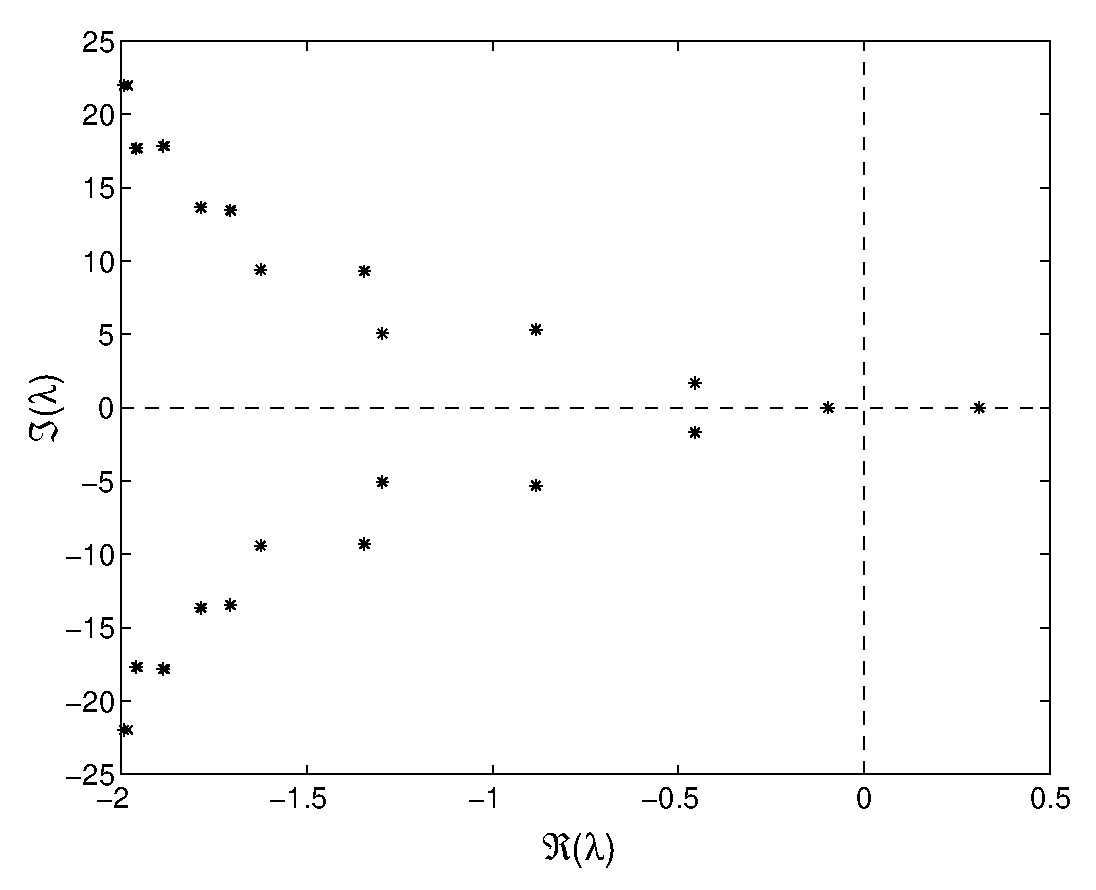
\includegraphics{fig/fig2.eps}}
\end{center}
\caption{\small\label{ride1+2_pic}Approximated $(\times)$
and corrected $(*)$ roots of the characteristic equation
of system (\ref{example_sys}) 
at its steady state solution $(x_1^*,x_2^*)=(0,0)$. 
Real parts computed up to $\Re(\lambda)\geq -\frac{1}{\tau}$
(left), $\Re(\lambda)\geq -2$ (right).} 
\end{figure}
We get default point method parameters and 
correct the point,
{\small\begin{verbatim}
>> method=df_mthod('stst')
method = continuation: [1x1 struct]
                point: [1x1 struct]
            stability: [1x1 struct]
>> [stst,success]=p_correc(stst,[],[],method.point)
stst = kind: 'stst'
  parameter: [0.5000 -1 1 2.3400 0.2000 0.2000 1.5000]
          x: [2x1 double]
success = 1
>> stst.x
ans = 0
      0
\end{verbatim}}
\noindent which, being already a correct solution, remains unchanged.
Computing and plotting stability of the corrected point reveals 
it has one unstable real mode, see figure \ref{ride1+2_pic} (left).
{\small\begin{verbatim}
>> stst.stability=p_stabil(stst,method.stability);
>> figure(1); clf;
>> p_splot(stst);
\end{verbatim}}
Seeing that only a few characteristic roots were computed we 
set $\parm{minimal\_real\_part}$ to a more
negative value (it is default empty which means that 
roots are computed up to $\Re(\lambda)\geq-1/\tau$) and recompute 
stability to obtain figure \ref{ride1+2_pic} (right).
{\small\begin{verbatim}
>> method.stability.minimal_real_part=-2;
>> stst.stability=p_stabil(stst,method.stability);
>> figure(2); clf;
>> p_splot(stst);
\end{verbatim}}
\noindent In both figures, approximations $(\times)$ and corrections $(*)$
are nearly indistinguishable.

We will use this point as a first point to compute a branch
of steady state solutions. 
First, we obtain an empty branch with free parameter $a_{21}$
limited by $a_{21}\in[0,5]$ and $\Delta a_{21}\leq 0.2$ between
points.
{\small\begin{verbatim}
>> branch1=df_brnch(4,'stst')
branch1 = method: [1x1 struct]
       parameter: [1x1 struct]
           point: []
>> branch1.parameter
ans = free: 4
 min_bound: [3x2 double]
 max_bound: []
  max_step: []
>> branch1.parameter.min_bound
ans = 5  0
      6  0
      7  0
>> branch1.parameter.min_bound(4,:)=[4 0];
>> branch1.parameter.max_bound(1,:)=[4 5];
>> branch1.parameter.max_step(1,:)=[4 0.2];
\end{verbatim}}
To obtain
a second starting point we change  
parameter value $a_{21}$ slightly and correct again. 
{\small\begin{verbatim}
>> branch1.point=stst;
>> stst.parameter(4)=stst.parameter(4)+0.1;
>> [stst,success]=p_correc(stst,[],[],method.point);
>> branch1.point(2)=stst;
\end{verbatim}}
Because we know how the branch of steady state solutions
continued in $a_{21}$ looks like (it is constant at
$(x_1^*,x_2^*)=(0,0)$) we disable plotting during continuation
by setting the corresponding continuation method parameter to zero.
{\small\begin{verbatim}
>> branch1.method.continuation.plot=0;
\end{verbatim}}
With two starting points and suitable method parameters 
we are ready to continue the branch in parameter $a_{21}$ (number 4),
allowing it to vary in the interval $[0,5]$ using a maximum
stepsize of 0.2 and 
a maximum of 100 corrections.
{\small\begin{verbatim}
>> [branch1,s,f,r]=br_contn(branch1,100)
BR_CONTN warning: boundary hit.
branch1 = method: [1x1 struct]
       parameter: [1x1 struct]
           point: [1x16 struct]
s = 15
f = 0
r = 0
\end{verbatim}}
During continuation, 
sixteen points were successfully computed ($s=16$)
before the right boundary $a_{21}=5$ was hit (signalled by a warning). 
No corrections failed ($f=0$) and no computed points were later
rejected ($r=0$). Reversing the order of the branch points
allows to continue to the left.
{\small\begin{verbatim}
>> branch1=br_rvers(branch1);
>> [branch1,s,f,r]=br_contn(branch1,100);
BR_CONTN warning: boundary hit.
\end{verbatim}}
We compute the stability along the branch.
{\small\begin{verbatim}
>> branch1.method.stability.minimal_real_part=-2;
>> branch1=br_stabl(branch1,0,1);
\end{verbatim}}
After obtaining suitable measure structures
we plot the real part of the approximated and corrected 
roots of the
characteristic equation along the branch, see figure
\ref{ride3+4_pic} (left). 
{\small\begin{verbatim}
>> [xm,ym]=df_measr(1,branch1);
>> figure(3); clf;
>> br_plot(branch1,xm,ym,'b');
>> ym
ym = field: 'stability'
  subfield: 'l1'
       row: 'all'
       col: 1
      func: 'real'
>> ym.subfield='l0';
>> br_plot(branch1,xm,ym,'c');
>> plot([0 5],[0 0],'-.');
>> axis([0 5 -2 1.5]);
\end{verbatim}}
Again approximations and 
corrections are nearly indistinguishable. From this figure alone it
is not clear which real parts correspond to real roots respectively
complex pairs of roots. For this it is 
useful to compare figures \ref{ride1+2_pic} and \ref{ride3+4_pic} (left).
Notice the strange behaviour (coinciding of several complex pairs
of roots) at $a_{21}=0$. At this parameter value
one of the couplings between the neurons is broken.
In fact, for $a_{21}=0$, the evolution of the second component is independent of
the evolution of the first. 
\begin{figure}[h]
\begin{center}
\resizebox{6cm}{!}{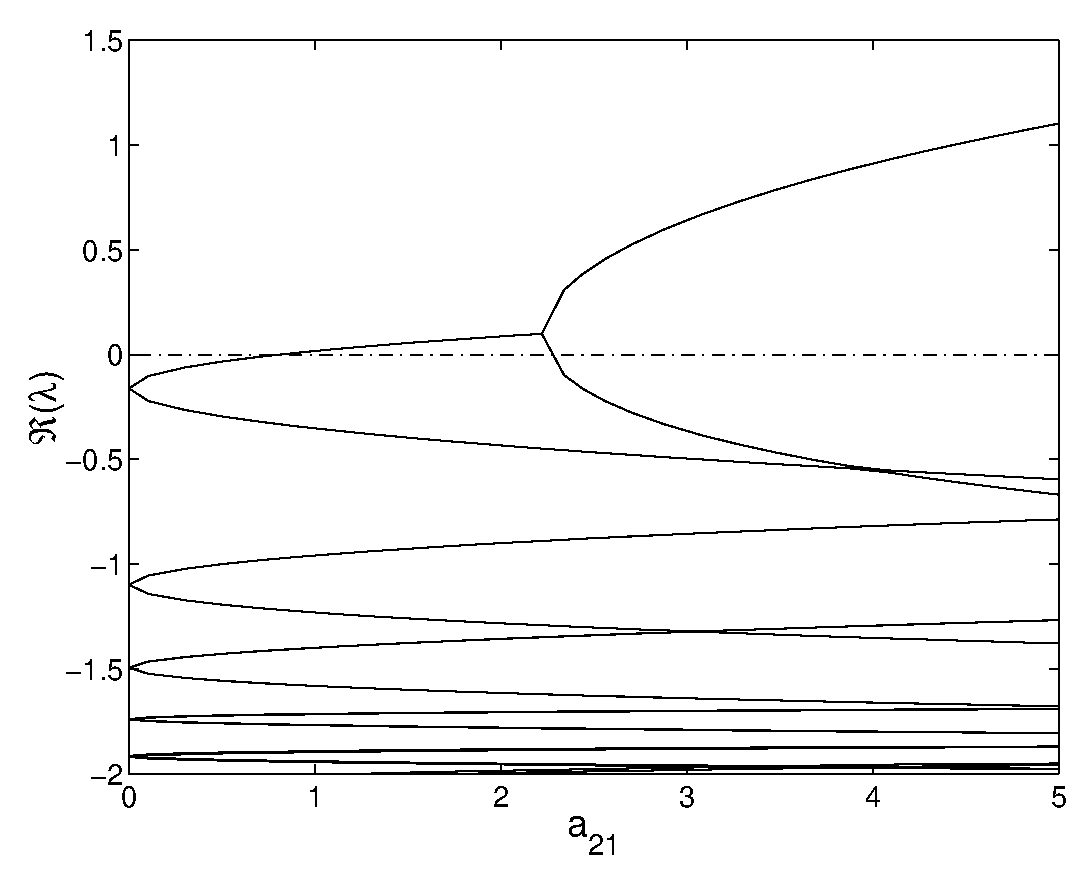
\includegraphics{fig/fig3.eps}}
\resizebox{6cm}{!}{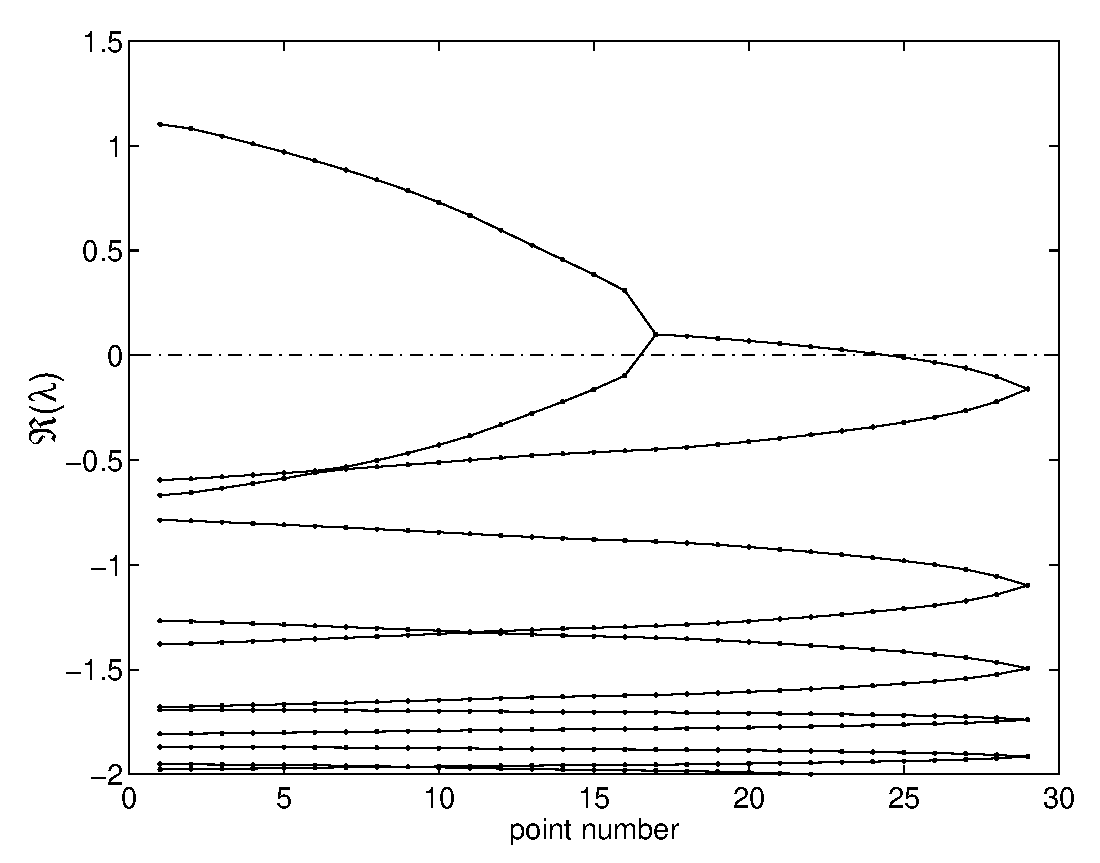
\includegraphics{fig/fig4.eps}}
\end{center}
\caption{\small\label{ride3+4_pic}Real parts of
the approximated (left) and corrected (left,right)
roots of the characteristic equation
versus $a_{21}$ (left) respectively the point number along the branch
(right).} 
\end{figure}
Where lines cross the zero line, bifurcations occur. If we want to 
compute the Hopf bifurcation near $a_{21}\approx0.8$ we need its point
number. This is most easily obtained by plotting the stability versus
the point numbers along the branch, see figure \ref{ride3+4_pic} (right).
{\small\begin{verbatim}
>> figure(4); clf;
>> br_plot(branch1,[],ym,'b');
>> br_plot(branch1,[],ym,'b.');
>> plot([0 30],[0 0],'-.');
\end{verbatim}}
We select point 24 and turn it into an (approximate) Hopf bifurcation point.
{\small\begin{verbatim}
>> hopf=p_tohopf(branch1.point(24));
\end{verbatim}}
\begin{figure}[h]
\begin{center}
\resizebox{7cm}{!}{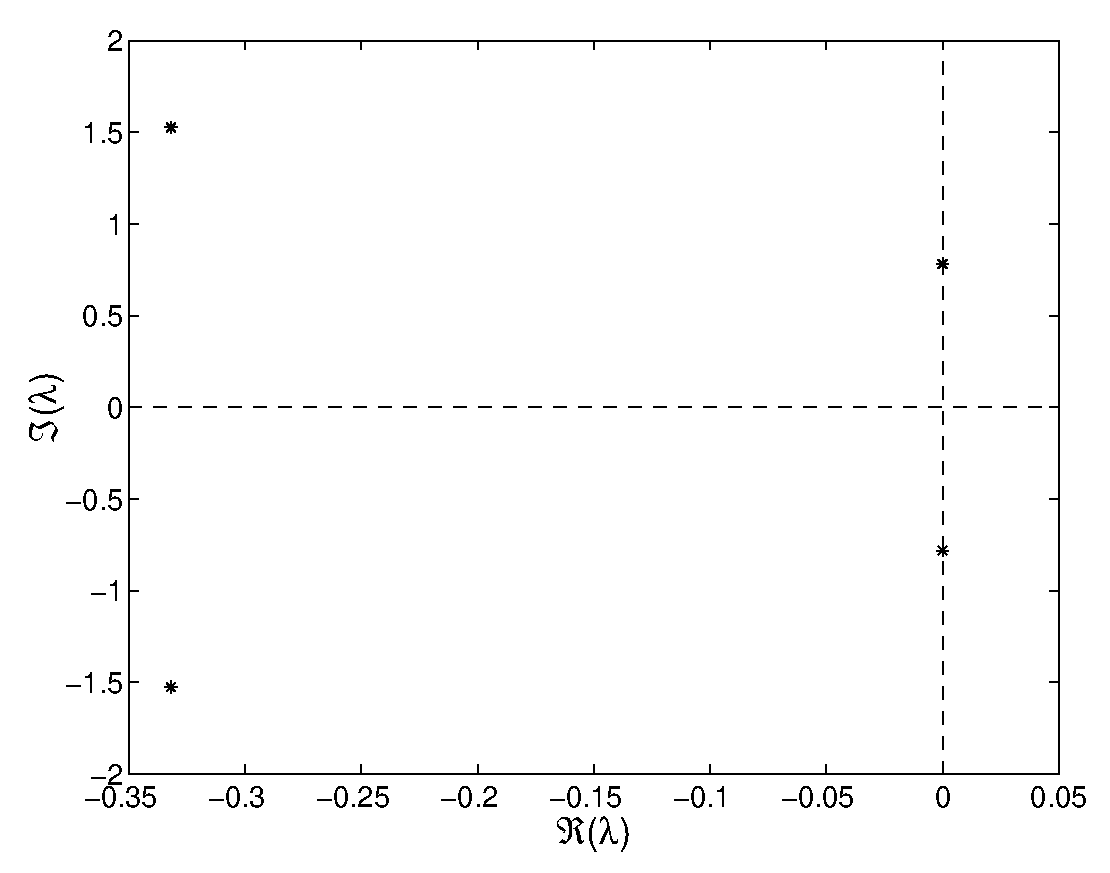
\includegraphics{fig/fig5.eps}}
\end{center}
\caption{\small\label{ride5_pic}Characteristic roots at Hopf
point: a pair of pure imaginary eigenvalues is clearly visible.} 
\end{figure}
We correct the Hopf point using appropriate method parameters
and one free parameter ($a_{21}$). We then copy the corrected point
to keep it for later use.
{\small\begin{verbatim}
>> method=df_mthod('hopf');
>> [hopf,success]=p_correc(hopf,4,[],method.point)
hopf = kind: 'hopf'
  parameter: [0.5000 -1 1 0.8071 0.2000 0.2000 1.5000]
          x: [2x1 double]
          v: [2x1 double]
      omega: 0.7820
success = 1
>> first_hopf=hopf;
\end{verbatim}}
Computing and plotting stability of the Hopf point clearly reveals the pair of pure
imaginary eigenvalues, see figure \ref{ride5_pic} 
{\small\begin{verbatim}
>> hopf.stability=p_stabil(hopf,method.stability);
>> figure(5); clf;
>> p_splot(hopf);
\end{verbatim}}
In order to follow a branch of Hopf bifurcations in the two parameter
space $(a_{21},\tau_s)$ we again need two starting points.
Hence we use the Hopf point already found and one perturbed in $\tau_s$
and corrected in $a_{21}$, to start on a branch
of Hopf bifurcations.
For the free parameters, $a_{21}$ and $\tau_s$, 
we provide suitable intervals, 
$a_{21}\in[0,4]$ and $\tau_s\in[0,10]$, and maximal stepsizes,
$0.2$ for $a_{21}$ and $0.5$ for $\tau_s$.
{\small\begin{verbatim}
>> branch2=df_brnch([4 7],'hopf');
>> branch2.parameter.min_bound(4,:)=[4 0];
>> branch2.parameter.max_bound(1:2,:)=[[4 4]' [7 10]']';
>> branch2.parameter.max_step(1:2,:)=[[4 0.2]' [7 0.5]']';
>> branch2.point=hopf;
>> hopf.parameter(7)=hopf.parameter(7)+0.1;
>> [hopf,success]=p_correc(hopf,4,[],method.point);
>> branch2.point(2)=hopf;
\end{verbatim}}
We continue the branch on both sides by an intermediate order
reversal and a second call to \file{br\_contn}.
{\small\begin{verbatim}
>> figure(6); clf;
>> [branch2,s,f,r]=br_contn(branch2,40);
BR_CONTN warning: boundary hit.
>> branch2=br_rvers(branch2);
>> [branch2,s,f,r]=br_contn(branch2,20);
\end{verbatim}}
\begin{figure}[h]
\begin{center}
\resizebox{6cm}{!}{\includegraphics{fig/fig6a.eps}}
\resizebox{6cm}{!}{\includegraphics{fig/fig6b.eps}}
\end{center}
\caption{\small\label{ride6_pic}Predictions and corrections
in the $(a_{21},\tau_s)$-plane after computation of a first
branch of Hopf bifurcations (left) and a second, intersecting
branch of Hopf bifurcations (right).} 
\end{figure}
As we did not change continuation method parameters,
predictions and corrections will be plotted during continuation.
The final result is shown in figure \ref{ride6_pic} (left).
At the top, the branch hits the boundary $\tau_s=10$. To the right, however,
it seemingly turned back onto itself.
We compute and plot stability along the branch.
{\small\begin{verbatim}
>> branch2=br_stabl(branch2,0,0);
>> figure(7); clf;
>> [xm,ym]=df_measr(1,branch2);
>> ym.subfield='l0';
>> br_plot(branch2,[],ym,'c');
>> ym.subfield='l1';
>> br_plot(branch2,[],ym,'b');
\end{verbatim}}
If, during these computations we would have obtained warnings of the kind,
{\small\begin{verbatim}
TIME_H warning: h_min is reached.
\end{verbatim}}
\noindent it would indicate that the time integration step required to obtain good
approximations to the requested rightmost characteristic roots 
is too small.
By default, characteristic roots are computed 
up to $\Re(\lambda)\geq-1/\tau$.
%This is clearly visible in the result, figure \ref{ride7+8_pic} (left). At the
%left side of the figure,
%the number of roots become
%too large for accurate approximations and the approximate characteristic roots 
%differ largely
%from the corrections. Notice that for smaller real parts the accuracy is still
%acceptable. In particular the pair of pure imaginary eigenvalues is present
%everywhere as a constant line at zero.

We also notice a double Hopf point on the left but nothing special at the
right end, which could explain the observed turning of the branch.
Plotting the frequency $\omega$ versus $\tau_s$ reveals what has happened,
see figure \ref{ride7+8_pic} (right).
For small $\tau_s$, $\omega$ goes through zero, indicating the presence
of a Bogdanov-Takens point. The subsequent turning is a recomputation
of the same branch with negative frequencies.
{\small\begin{verbatim}
>> figure(8); clf;
>> [xm,ym]=df_measr(0,branch2);
>> ym
ym = field: 'parameter'
  subfield: ''
       row: 1
       col: 7
      func: ''
>> ym.field='omega';
>> ym.col=1;
>> xm
xm = field: 'parameter'
  subfield: ''
       row: 1
       col: 4
      func: ''
>> xm.col=7;
>> br_plot(branch2,xm,ym,'c');
>> grid;
\end{verbatim}}
\begin{figure}[h]
\begin{center}
\resizebox{6cm}{!}{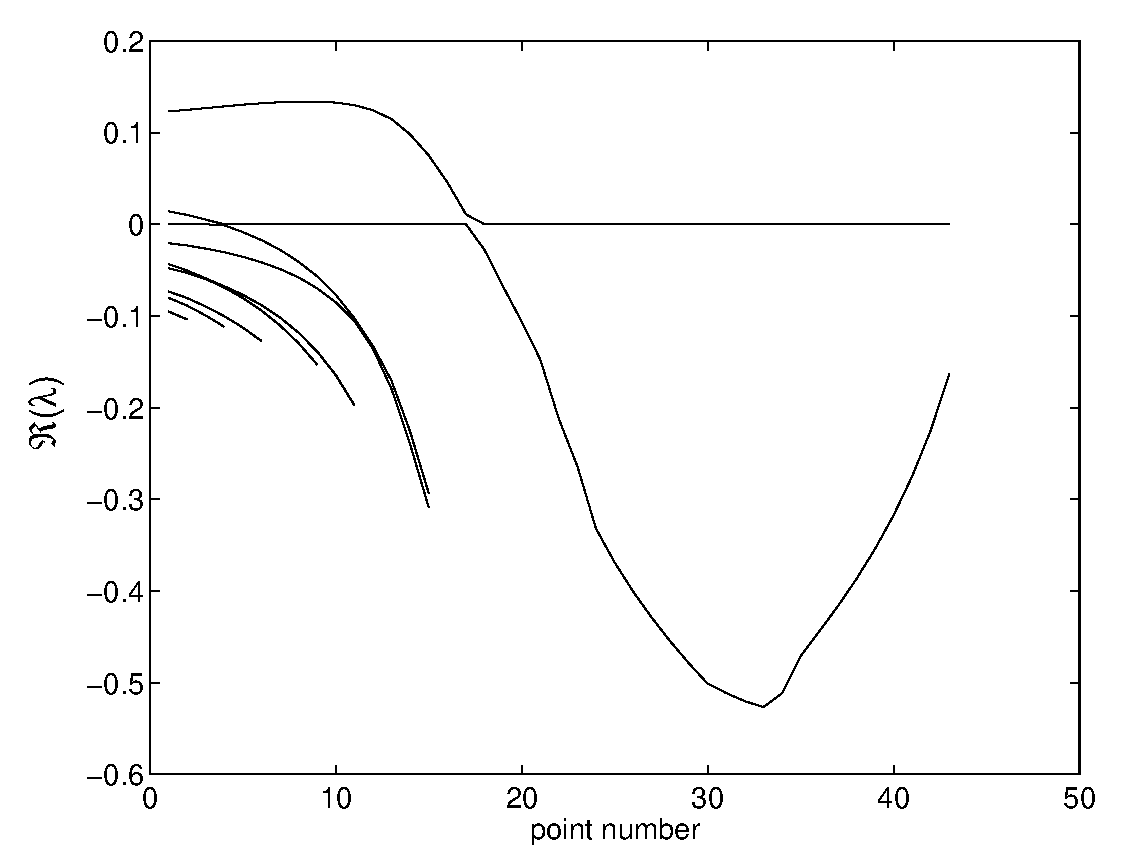
\includegraphics{fig/fig7.eps}}
\resizebox{6cm}{!}{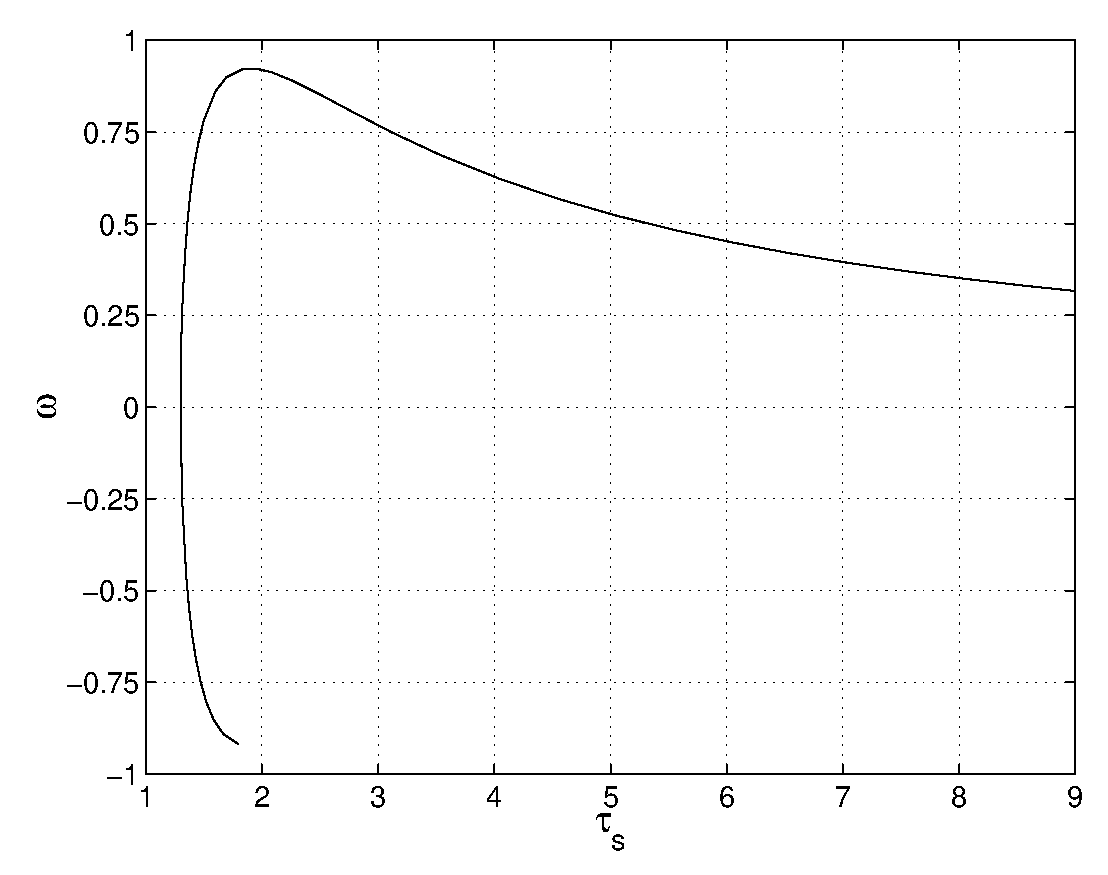
\includegraphics{fig/fig8.eps}}
\end{center}
\caption{\small\label{ride7+8_pic}Left:
Real part of characteristic roots along the branch of Hopf
bifurcations shown in figure \ref{ride6_pic} (left). Right:
The frequency of the Hopf bifurcation along the same branch.} 
\end{figure}
Selecting the double Hopf point we produce an approximation of the
second Hopf point.
{\small\begin{verbatim}
>> hopf=p_tohopf(branch2.point(4));
>> [hopf,success]=p_correc(hopf,4,[],method.point)
hopf = kind: 'hopf'
  parameter: [0.5000 -1 1 -0.0103 0.2000 0.2000 8.5530]
          x: [2x1 double]
          v: [2x1 double]
      omega: 0.9768
success = 0
\end{verbatim}}
However, without success. Printing residual information
gives a list of the Newton iteration number and the
norm of the residual. This reveals 
at least temporarily divergence
of the correction process.
{\small\begin{verbatim}
>> method.point.print_residual_info=1;
>> format short e;
>> hopf=p_tohopf(branch2.point(4));
>> [hopf,success]=p_correc(hopf,4,[],method.point);
norm_residual = 1.0000e+00  9.3116e-03
norm_residual = 2.0000e+00  5.4574e-01
norm_residual = 3.0000e+00  6.2629e-02
norm_residual = 4.0000e+00  1.8903e-03
norm_residual = 5.0000e+00  3.2357e-05
\end{verbatim}}
Or we did not allow enough Newton iterations, or the free parameter
is not so appropriate.
We successfully try again using $\tau_s$ as a free parameter.
{\small\begin{verbatim}
>> hopf=p_tohopf(branch2.point(4));
>> [hopf,success]=p_correc(hopf,7,[],method.point)
norm_residual = 1.0000e+00   9.3116e-03
norm_residual = 2.0000e+00   6.8069e-04
norm_residual = 3.0000e+00   2.3169e-07
norm_residual = 4.0000e+00   4.3066e-13
hopf = kind: 'hopf'
  parameter: [5.0000e-01 -1 1 2.0657e-01 2.0000e-01 2.0000e-01 8.6340e+00]
          x: [2x1 double]
          v: [2x1 double]
      omega: 9.1581e-01
success = 1
\end{verbatim}}
Using the second Hopf point we compute the intersecting branch
of Hopf points depicted in figure \ref{ride6_pic} (right).
Setting $\parm{plot\_progress}$ to zero disables intermediate plotting
such that we see only the end result.
{\small\begin{verbatim}
>> branch3=df_brnch([4 7],'hopf');
>> branch3.parameter=branch2.parameter;
>> branch3.point=hopf;
>> hopf.parameter(4)=hopf.parameter(4)-0.05;
>> method.point.print_residual_info=0; format short;
>> [hopf,success]=p_correc(hopf,7,[],method.point);
>> branch3.point(2)=hopf;
>> branch3.method.continuation.plot_progress=0;
>> figure(6);
>> [branch3,s,f,r]=br_contn(branch3,100);
BR_CONTN warning: boundary hit.
>> branch3=br_rvers(branch3);
>> [branch3,s,f,r]=br_contn(branch3,100);
BR_CONTN warning: boundary hit.
\end{verbatim}}
We use the first Hopf point we computed ($\parm{first\_hopf}$)
to construct a small amplitude ($1e-2$)
periodic solution on an equidistant mesh of
$18$ intervals with piecewise polynomial degree $3$.
{\small\begin{verbatim}
>> intervals=18;
>> degree=3;
>> [psol,stepcond]=p_topsol(first_hopf,1e-2,degree,intervals);
\end{verbatim}}
This steplength condition returned ensures the branch switch from the
Hopf to the periodic solution as it avoids convergence of  
the amplitude 
to zero during corrections. Due to the presence of the
steplength condition we also need to
free one parameter, here $a_{21}$.
{\small\begin{verbatim}
>> method=df_mthod('psol');
>> [psol,success]=p_correc(psol,4,stepcond,method.point)
psol = kind: 'psol'
  parameter: [0.5000 -1 1 0.8072 0.2000 0.2000 1.5000]
       mesh: [1x55 double]
     degree: 3
    profile: [2x55 double]
     period: 8.0354
success = 1
\end{verbatim}}
The result, along with a degenerate periodic solution with amplitude
zero is used to start on the emanating branch of periodic solutions,
see figure \ref{ride9_pic} (left). We avoid adaptive 
mesh selection and save memory by clearing the mesh field. 
An equidistant mesh is then automatically used which is kept
fixed during continuation. Simple clearing of the mesh field
is only  possible if it is already equidistant. This is the case
here as \file{p\_tohopf} returns a solution on an
equidistant mesh. 
{\small\begin{verbatim}
>> branch4=df_brnch(4,'psol');
>> branch4.parameter.min_bound(4,:)=[4 0];
>> branch4.parameter.max_bound(1,:)=[4 5];
>> branch4.parameter.max_step(1,:)=[4 0.1];
>> deg_psol=p_topsol(first_hopf,0,degree,intervals);
>> deg_psol.mesh=[];
>> branch4.point=deg_psol;
>> psol.mesh=[];
>> branch4.point(2)=psol;
>> figure(9); clf;
>> [branch4,s,f,r]=br_contn(branch4,50);
\end{verbatim}}
Notice how computing periodic solution branches takes 
considerably more
computational time.
Zooming shows erratic behaviour of the last computed 
branch points, shortly beyond a turning point, see figure \ref{ride9_pic} (right).
{\small\begin{verbatim}
>> axis([2.3 2.4 0.95 1.15]);
\end{verbatim}}
\begin{figure}[h]
\begin{center}
\resizebox{6cm}{!}{\includegraphics{fig/fig9a.eps}}
\resizebox{6cm}{!}{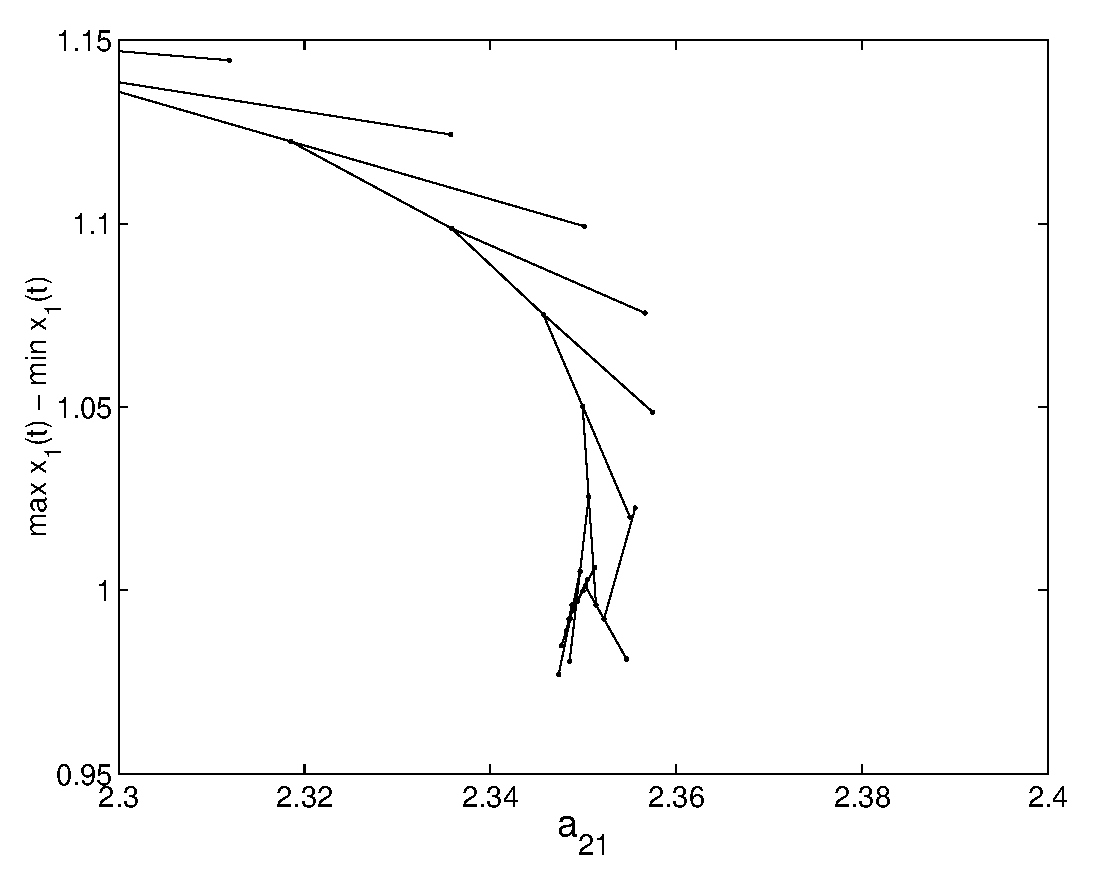
\includegraphics{fig/fig9b.eps}}
\end{center}
\caption{\small\label{ride9_pic}Branch of periodic solutions emanating
from a Hopf point (left). The branch turns at the far right and a zoom (right)
indicates computational difficulties at the end.} 
\end{figure}
Plotting some of the last solution profiles shows that smoothness
and thus also accuracy are lost, see figure \ref{ride10+13_pic} (left).
{\small\begin{verbatim}
>> ll=length(branch4.point);
>> figure(10); clf;
>> subplot(3,1,1);
>> p_pplot(branch4.point(ll-10));
>> subplot(3,1,2);
>> p_pplot(branch4.point(ll-5));
>> subplot(3,1,3);
>> p_pplot(branch4.point(ll-1));
\end{verbatim}}
From a plot of the period along the branch we could suspect a homoclinic
or heteroclinic bifurcation scenario, see figure \ref{ride11_pic} (left).
\begin{figure}[h]
\begin{center}
\resizebox{6cm}{!}{\includegraphics{fig/fig11a.eps}}
\resizebox{6cm}{!}{\includegraphics{fig/fig11b.eps}}
\end{center}
\caption{\small\label{ride11_pic}Left: Period along the
computed branch shown in figure \ref{ride9_pic}. Right: Added period
predictions and corrections during recalculations using
adaptive mesh selection.} 
\end{figure}
{\small\begin{verbatim}
>> figure(11); clf;
>> [xm,ym]=df_measr(0,branch4);
>> ym
ym = field: 'profile'
  subfield: ''
       row: 1
       col: 'ampl'
      func: ''
>> ym.field='period';
>> ym.col=1;
>> br_plot(branch4,xm,ym,'b');
>> axis([2.2 2.36 20 170]);
\end{verbatim}}
\begin{figure}[h]
\begin{center}
\resizebox{6cm}{!}{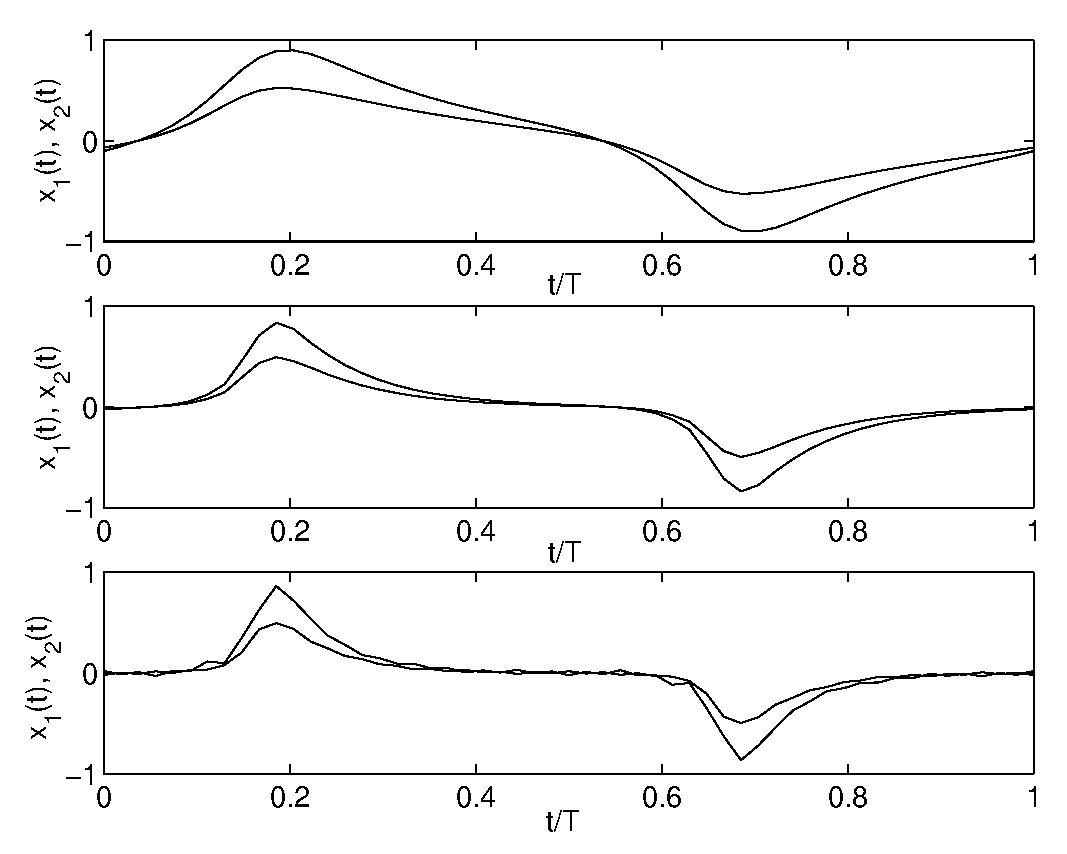
\includegraphics{fig/fig10.eps}}
\resizebox{6cm}{!}{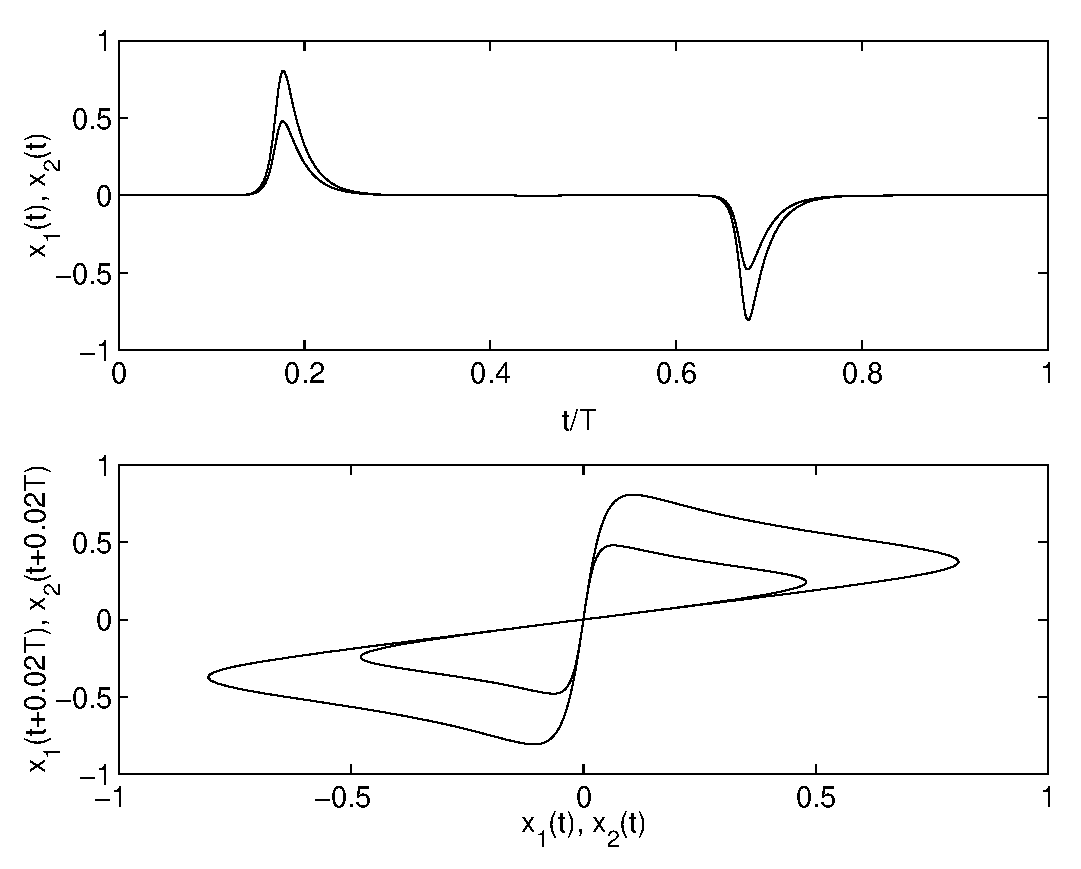
\includegraphics{fig/fig13.eps}}
\end{center}
\caption{\small\label{ride10+13_pic}Some solution profiles
using equidistant meshes (left) and adapted meshes right (right) 
along the branch of periodic solutions 
shown in figure \ref{ride9_pic}.} 
\end{figure}
The result of computing and plotting stability (Floquet multipliers) 
just before
and after the turning point is shown in figure \ref{ride12_pic}. 
The second spectrum is clearly unstable but no accurate trivial
Floquet multiplier is present at 1. 
{\small\begin{verbatim}
>> psol=branch4.point(ll-11);
>> psol.stability=p_stabil(psol,method.stability);
>> figure(12); clf;
>> subplot(2,1,1);
>> p_splot(psol);
>> axis image;
>> psol=branch4.point(ll-8);
>> psol.stability=p_stabil(psol,method.stability);
>> subplot(2,1,2);
>> p_splot(psol);
\end{verbatim}}
\begin{figure}[h]
\begin{center}
\resizebox{6cm}{!}{\includegraphics{fig/fig12.eps}}
\end{center}
\caption{\small\label{ride12_pic}Floquet multipliers for
a periodic solutions before (top) and just after (bottom)
the turning point visible in figure \ref{ride9_pic}.}
\end{figure}
First, we recompute a point on a refined, adapted mesh.
{\small\begin{verbatim}
>> psol=branch4.point(ll-12);
>> intervals=40;
>> degree=4;
>> psol=p_remesh(psol,degree,intervals);
>> method.point.adapt_mesh_after_correct=1;
>> method.point.newton_max_iterations=7;
>> method.point.newton_nmon_iterations=2;
>> [psol,success]=p_correc(psol,[],[],method.point)
psol = kind: 'psol'
  parameter: [0.5000 -1 1 2.3358 0.2000 0.2000 1.5000]
       mesh: [1x161 double]
     degree: 4
    profile: [2x161 double]
     period: 38.4916
success = 1
\end{verbatim}}
Then we recompute the branch using adaptive mesh selection
(with reinterpolation and additional corrections) 
after correcting every point, see figure \ref{ride11_pic} (right).
{\small\begin{verbatim}
>> branch5=df_brnch(4,'psol');
>> branch5.parameter=branch4.parameter;
>> branch5.point=psol;
>> psol.parameter(4)=psol.parameter(4)+0.01;
>> [psol,success]=p_correc(psol,[],[],method.point,1);
>> branch5.point(2)=psol;
>> branch5.method=method;
>> [xm,ym]=df_measr(0,branch5);
>> ym.field='period';
>> ym.col=1;
>> figure(11); axis auto; hold on;
>> branch5.method.continuation.plot_measure.x=xm;
>> branch5.method.continuation.plot_measure.y=ym;
>> branch5=br_contn(branch5,25);
\end{verbatim}}
Increasing mesh sizes and using adaptive mesh selection
also improves the accuracy of the computed Floquet multipliers.
{\small\begin{verbatim}
>> psol=branch5.point(6);
>> psol.stability=p_stabil(psol,method.stability);
>> psol.stability.mu 
ans = 241.2300
        1.0000
\end{verbatim}}
Plotting of a point clearly shows the (double)
homoclinic nature of the solutions, see figure \ref{ride10+13_pic} (right).
{\small\begin{verbatim}
>> figure(13); clf;
>> subplot(2,1,1);
>> ll=length(branch5.point);
>> psol=branch5.point(ll-5);
>> plot(psol.mesh,psol.profile);
>> subplot(2,1,2);
>> psol1=p_remesh(psol,degree,0:0.001:1);
>> psol2=p_remesh(psol,degree,(0:0.001:1)+0.02);
>> plot(psol1.profile',psol2.profile');
>> psol.period
ans = 399.7466
\end{verbatim}}
%Ending this section and the Matlab session 
%reveals a rather large number of operations performed during
%the calculations described.
%{\small\begin{verbatim}  
%>> exit 
%6114113212 flops.
%\end{verbatim}}
In this case, using the file \file{df\_deriv.m} instead of the 
analytical derivatives file given in section \ref{sys_def1},
yields results which are visually the same as the ones given
above.
%{\small\begin{verbatim}  
%7169739860 flops.
%\end{verbatim}}

Using the (added) routines to compute homoclinic solutions, we
correct each of the two loops to a homoclinic orbit, thereby obtaining
also some stability information of the steady state point.
We take the first half of the profile and rescale it to $[0,1]$.
{\small\begin{verbatim}
>> figure(14);clf;subplot(2,1,1);
>> hcli1=psol;
>> hcli1.mesh=hcli1.mesh(1:65);
>> hcli1.profile=hcli1.profile(:,1:65);
>> hcli1.period=hcli1.period*hcli1.mesh(end);
>> hcli1.mesh=hcli1.mesh/hcli1.mesh(end);
\end{verbatim}}
Now we convert this point to a point of kind 'hcli' and correct it.
{\small\begin{verbatim}
>> hcli1=p_tohcli(hcli1)
hcli1 = kind: 'hcli'
    parameter: [0.5000 -1 1 2.3460 0.2000 0.2000 1.5000]
         mesh: [1x61 double]
       degree: 4
      profile: [2x61 double]
       period: 113.4318
           x1: [2x1 double]
           x2: [2x1 double]
     lambda_v: 0.3142
     lambda_w: 0.3142
            v: [2x1 double]
            w: [2x1 double]
        alpha: 1
      epsilon: 2.9010e-04
>> mh=df_mthod('hcli');
>> [hcli1,success]=p_correc(hcli1,4,[],mh.point)
hcli1 =  kind: 'hcli'
    parameter: [0.5000 -1 1 2.3459 0.2000 0.2000 1.5000]
         mesh: [1x61 double]
       degree: 4
      profile: [2x61 double]
       period: 114.8378
           x1: [2x1 double]
           x2: [2x1 double]
     lambda_v: 0.3141
     lambda_w: 0.3141
            v: [2x1 double]
            w: [2x1 double]
        alpha: 1
      epsilon: 2.9010e-04
success = 1
>> p_pplot(hcli1);
\end{verbatim}}

We apply the same procedure on the second half of the profile.
{\small\begin{verbatim}
>> figure(14);subplot(2,1,2);
>> hcli2=psol;
>> hcli2.mesh=hcli2.mesh(81:end-16);
>> hcli2.profile=hcli2.profile(:,81:end-16);
>> hcli2.mesh=hcli2.mesh-hcli2.mesh(1);
>> hcli2.period=hcli2.period*hcli2.mesh(end);
>> hcli2.mesh=hcli2.mesh/hcli2.mesh(end);
>> hcli2=p_tohcli(hcli2);
>> [hcli2,success]=p_correc(hcli2,4,[],mh.point);
>> p_pplot(hcli2);
\end{verbatim}}
\begin{figure}[h]
\begin{center}
\resizebox{6cm}{!}{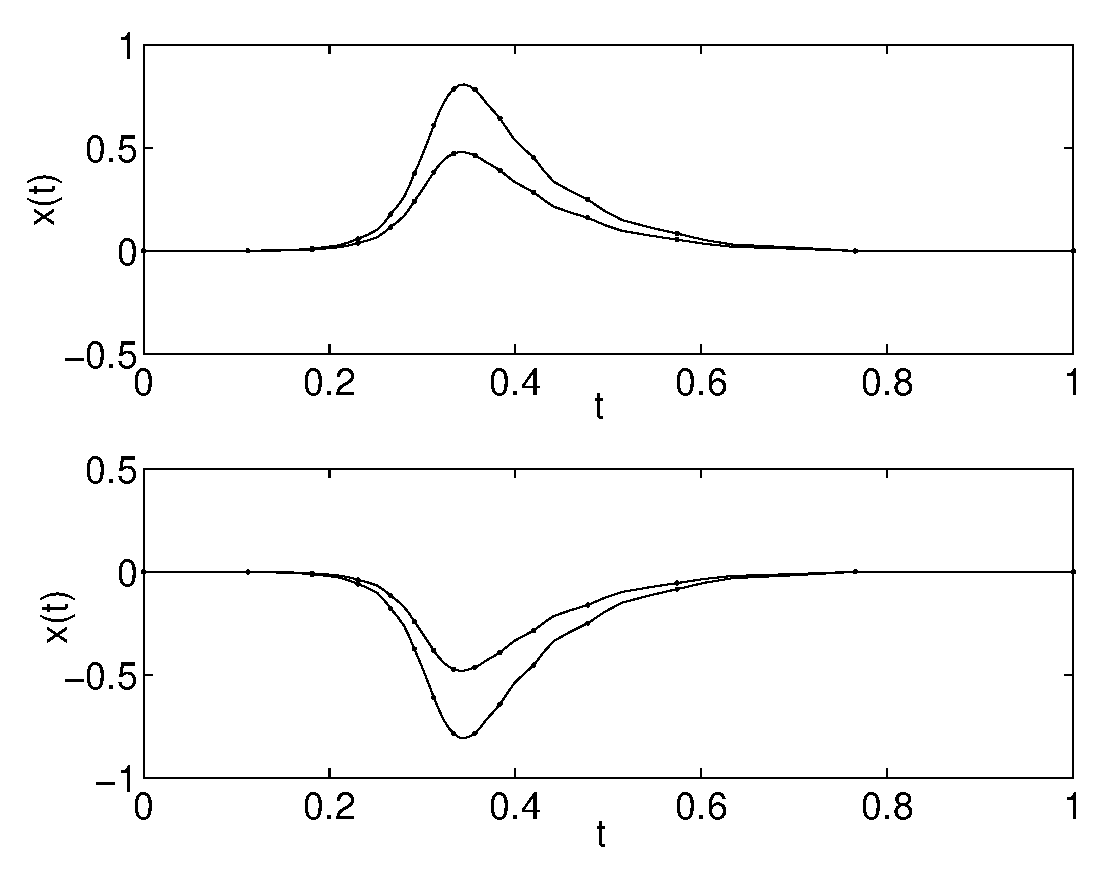
\includegraphics{fig/fig14.eps}}
\end{center}
\caption{\small\label{ride14_pic}Homoclinic profiles of the two loops
depicted in figure \ref{ride10+13_pic}.}
\end{figure}
We recompute the first homoclinic orbit, using 70 intervals, and correct this point.
{\small\begin{verbatim}
>> hcli1=p_remesh(hcli1,4,70);
>> [hcli1,success]=p_correc(hcli1,4,[],mh.point)
hcli1 = kind: 'hcli'
    parameter: [0.5000 -1 1 2.3460 0.2000 0.2000 1.5000]
         mesh: [1x281 double]
       degree: 4
      profile: [2x281 double]
       period: 115.5581
           x1: [2x1 double]
           x2: [2x1 double]
     lambda_v: 0.3142
     lambda_w: 0.3142
            v: [2x1 double]
            w: [2x1 double]
        alpha: 1
      epsilon: 2.9010e-04
success = 1
\end{verbatim}}
If we free a second parameter, we can continue this homoclinic orbit with 
respect to two free parameters.  As a second free parameter, 
we choose $\tau_s$. We first create a default branch of homoclinic orbits,
add \verb#hcli1# as a first point, perturb it, and add the corrected
perturbation as a second point.
{\small\begin{verbatim}
>> figure(15);
>> branch6=df_brnch([4 7],'hcli');
>> branch6.point=hcli1;
>> hcli1.parameter(7)=1.49;
>> [hcli1,success]=p_correc(hcli1,4,[],mh.point);
>> branch6.point(2)=hcli1;
>> [branch6,s,r,f]=br_contn(branch6,19);
\end{verbatim}} 
\begin{figure}[h]
\begin{center}
\resizebox{6cm}{!}{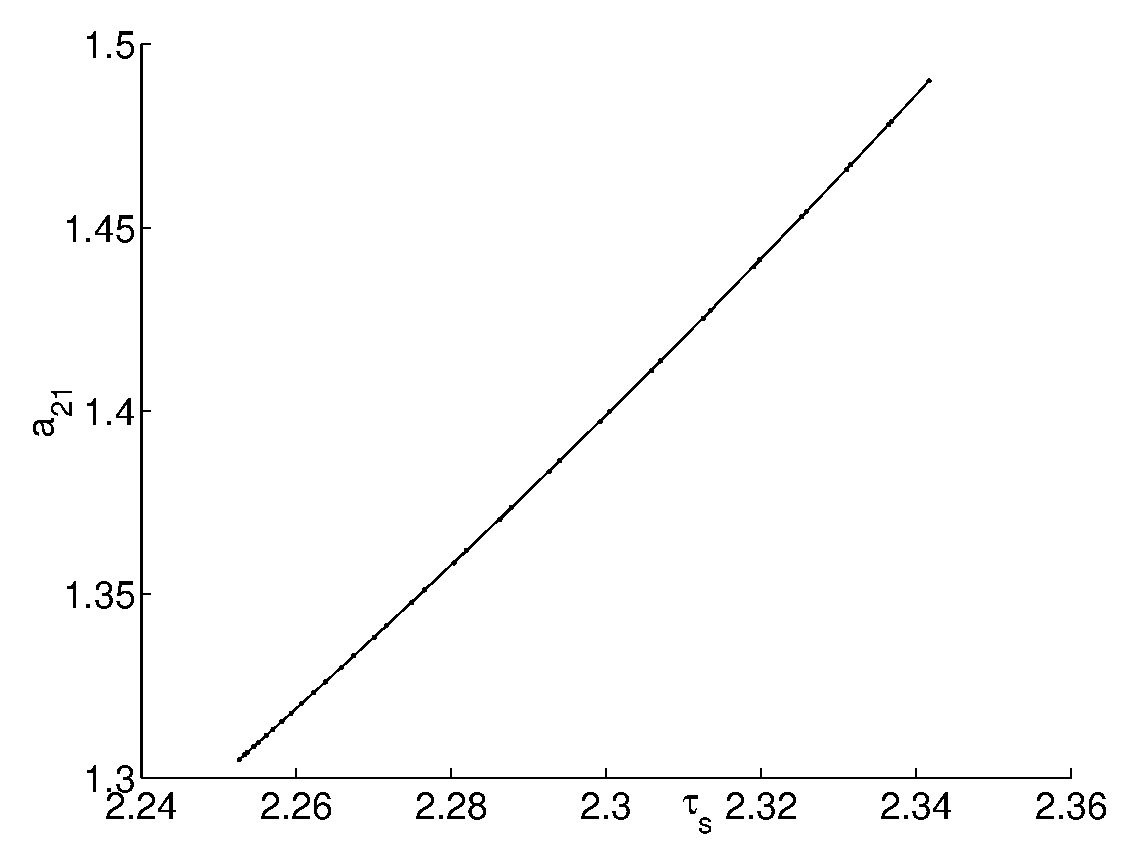
\includegraphics{fig/fig15.eps}}
\end{center}
\caption{\small\label{ride15_pic}Predictions and corrections in the 
($a_{21},\tau_s$)-plane after computation of a branch of homoclinic 
orbits.}
\end{figure}
%This example exhibits two symmetric homoclinic orbits.  This is not
%very generic, so in section~\ref{demo3} we will 
%discuss this type of continuation
%of homoclinic in a more detail in an other example system.
Because of the symmetry in this example, which is not generic, we choose to 
discuss continuation and analysis of branches of homoclinic orbits in a 
separate demo example.  We refer to section \ref{demo3}.

\subsection{sd-DDE demo: equations with (constant and) 
state-dependent delays}\label{demo2} 
This demo describes how to use \DDEBIFCODE\ to perform a 
bifurcation analysis on equations
with state-dependent delays.  System definitions files 
(see section \ref{sys_def2}) can be
found in the directory \verb$SD_DEMO$.  The commands used in this 
demo are listed in the file 
\file{sd\_demo.m}.

After the system has been implemented, bifurcation analysis can be performed.
Since the bifurcation analysis of
DDEs and sd-DDEs with the package is very similar, we do not provide
here an illustrative ride-through as in section \ref{ride-through}.
Using the example~(\ref{example_sys2}), we perform the main steps of 
the analysis 
and show new elements related to the state dependency of delays.
The reader is recommended to read section \ref{ride-through} first, 
to be more familiar with the analysis.

The commands below are listed in the file \file{sd\_demo.m}.
The figures shown are produced during its execution. 

After starting Matlab in the directory of the system definition,
we install the system by calling its initialization file,
{\small\begin{verbatim}
>> [name,n]=sys_init
name = sd_demo
n = 5
\end{verbatim}}
We define a steady state solution using the
parameter values listed in $\parm{stst.parameter}$ and an initial
guess in $\parm{stst.x}$. Then we get default point method parameters 
and correct the point,
{\small\begin{verbatim}
>> stst.kind='stst';
>> stst.parameter=[4.5 0.04 -1.4 6 -0.45 -0.01 3 0.3 0.1 1 0.2];
>> stst.x=[[1.4 1.5 -25 0.6 1.4]';
>> method=df_mthod('stst');
>> [stst,success]=p_correc(stst,[],[],method.point)
stst = kind: 'stst'
  parameter: [1x11 double]
          x: [5x1 double]
success = 1
>> stst.x
ans = 1.4134
      1.5193
    -25.1077
      0.5886
      1.3801
\end{verbatim}}
We will use this point as a first point to compute a branch
of steady state solutions. 
First, we obtain an empty branch with free parameter $p_5$.
To obtain a second starting point we change parameter value $p_5$ 
slightly and correct again.

{\small\begin{verbatim}
>> branch1=df_brnch(5,'stst');
>> branch1.parameter.min_bound(1,:)=[5 -1];
>> branch1.parameter.max_bound(1,:)=[5 1];
>> branch1.parameter.max_step(1,:)=[5 0.1];    
>> branch1.point=stst;
>> stst.parameter(5)=stst.parameter(5)-0.01;
>> [stst,success]=p_correc(stst,[],[],method.point);
>> branch1.point(2)=stst;
\end{verbatim}}
With two starting points and suitable method parameters
we continue the branch (with plotting) versus parameter $p_5$,
see figure~\ref{br_stst} (left).
{\small\begin{verbatim}
>> figure(1); clf;
>> [branch1,s,f,r]=br_contn(branch1,20)
BR_CONTN warning: delay number_3 becomes negative.
branch1 = method: [1x1 struct]
       parameter: [1x1 struct]
           point: [1x9 struct]
s = 8
f = 0
r = 0
\end{verbatim}}

{\small\begin{verbatim}
>> plot(branch1.point(end).parameter(5),branch1.point(end).x(1),'o');
\end{verbatim}}

\begin{figure}[h]
\begin{center}
\resizebox{6cm}{!}{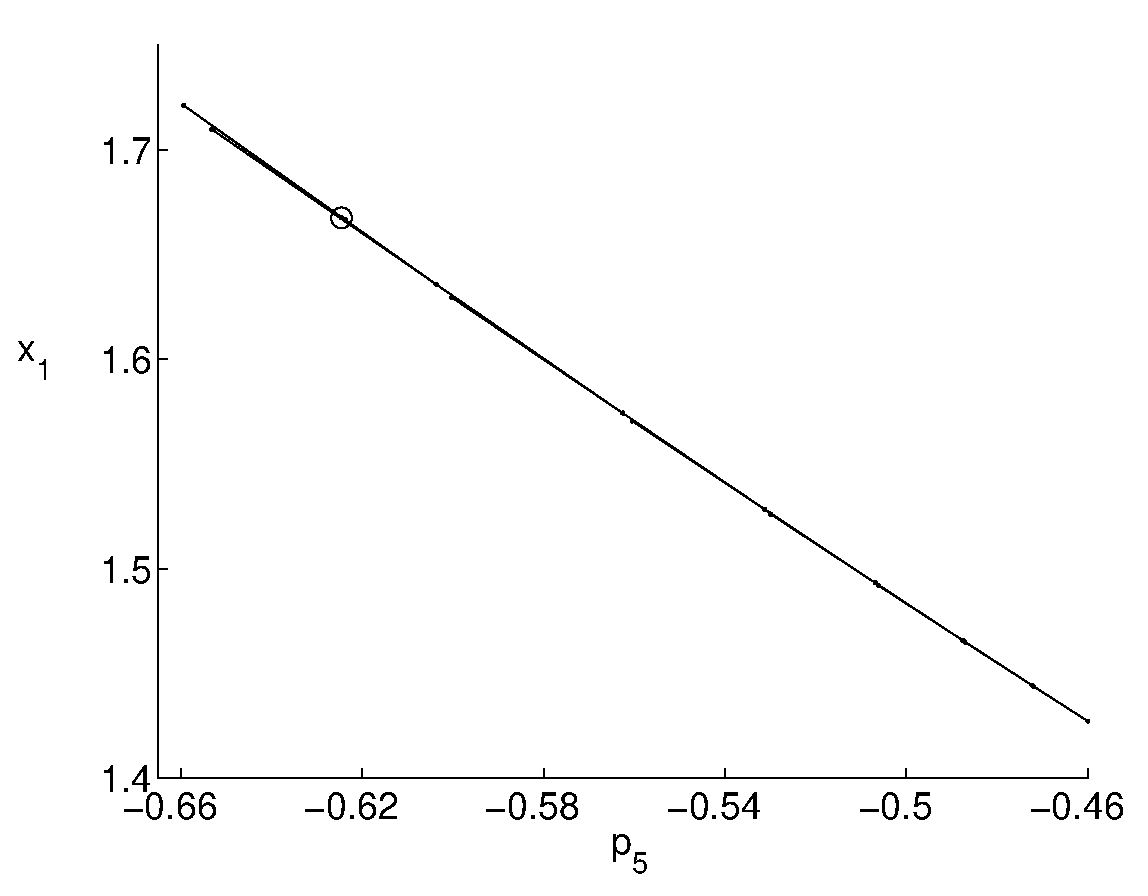
\includegraphics{fig/sdd1.eps}}
\resizebox{6cm}{!}{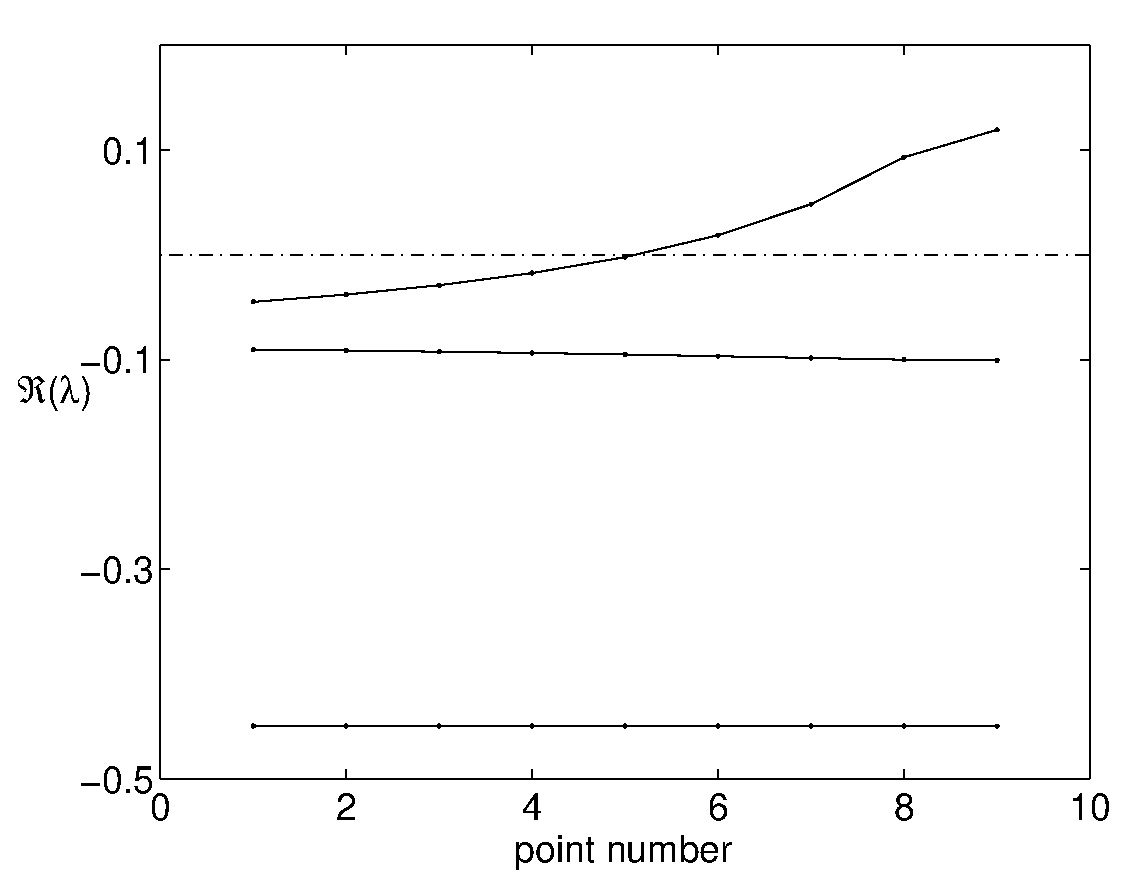
\includegraphics{fig/sdd2.eps}}
\end{center}
\caption{\small\label{br_stst} Left: predictions and corrections
after computation of a branch of steady state solutions versus
parameter $p_5$. $\circ$ - the last computed point in the branch
(corresponding to $\tau_3=0$). Right: Real parts of the corrected roots 
of the characteristic equation along the branch.}
\end{figure}

During continuation, seven points were successfully computed
before the state-dependent delay function $\tau_3$ crossed zero 
(signalled by a warning). 
The computed point with $\tau_3<0$ was not accepted. Instead, the point 
corresponding to $\tau_3=0$ was computed, see figure
\ref{br_stst} (left). We compute the value of $\tau_3$ at 
the last point in the branch:

{\small\begin{verbatim}
>> p_tau(branch1.point(end),3)
ans = 2.2204e-16
\end{verbatim}}
In similar cases, it might happen that the computed value of a delay is 
a very small negative value. 
Because stability cannot be computed when there are negative delays, 
small negative delay values are automatically neglected
when their value is larger than the value defined in
$\parm{method.stability.delay\_accuracy}$ (see table~\ref{meth_stab_struct}).

We compute the stability along the branch and after obtaining suitable 
measure structures we plot the real part of 
the corrected roots of the characteristic equation along the branch
versus the point numbers, see figure \ref{br_stst} (right).
{\small\begin{verbatim}
>> branch1.method.stability.minimal_real_part=-1;
>> branch1=br_stabl(branch1,0,0);
>> [xm,ym]=df_measr(1,branch1);
>> ym.subfield='l1';
>> figure(2); clf;
>> br_plot(branch1,[],ym,'b');
>> br_plot(branch1,[],ym,'b.');
>> plot([0 10],[0 0],'-.');
\end{verbatim}}

From this figure it is not clear which real parts correspond 
to real roots respectively complex pairs of roots. We check point 5,
{\small\begin{verbatim}
>> branch1.point(5).stability.l1
ans = -0.0023 - 0.5488i
      -0.0023 + 0.5488i
      -0.0952          
      -0.4499    
\end{verbatim}}

We select point 5 and turn it into an (approximate) Hopf-like 
bifurcation point.
{\small\begin{verbatim}
>> hopf=p_tohopf(branch1.point(5));
\end{verbatim}}
We correct the Hopf-like point using appropriate method parameters
and one free parameter ($p_5$). 
{\small\begin{verbatim}
>> method=df_mthod('hopf');
>> [hopf,success]=p_correc(hopf,5,[],method.point)
hopf = kind: 'hopf'
  parameter: [11x1 double]
          x: [5x1 double]
          v: [5x1 double]
      omega:0.5497 
success = 1
\end{verbatim}}
In order to follow a branch of Hopf-like bifurcations in the two parameter
space $(p_2,p_9)$ we again need two starting points.
We use the Hopf-like point already found and one perturbed in $p_9$
and corrected in $p_2$, to start on a branch
of Hopf-like bifurcations.
{\small\begin{verbatim}
>> branch2=df_brnch([2 9],'hopf');
>> branch2.parameter.min_bound(1:2,:)=[[2 -1]' [9 -1]']';
>> branch2.parameter.max_bound(1:2,:)=[[2 10]' [9 10]']';
>> branch2.parameter.max_step(1:2,:)=[[2 1]' [9 1]']';    
>> branch2.point=hopf;
>> hopf.parameter(9)=hopf.parameter(9)+0.1;
>> [hopf,success]=p_correc(hopf,2,[],method.point);
>> branch2.point(2)=hopf;
\end{verbatim}}
We continue the branch, see figure \ref{br_hopf}.
{\small\begin{verbatim}
>> figure(3); clf;
>> [branch2,s,f,r]=br_contn(branch2,14);
\end{verbatim}}
\begin{figure}[h]
\begin{center}
\resizebox{6cm}{!}{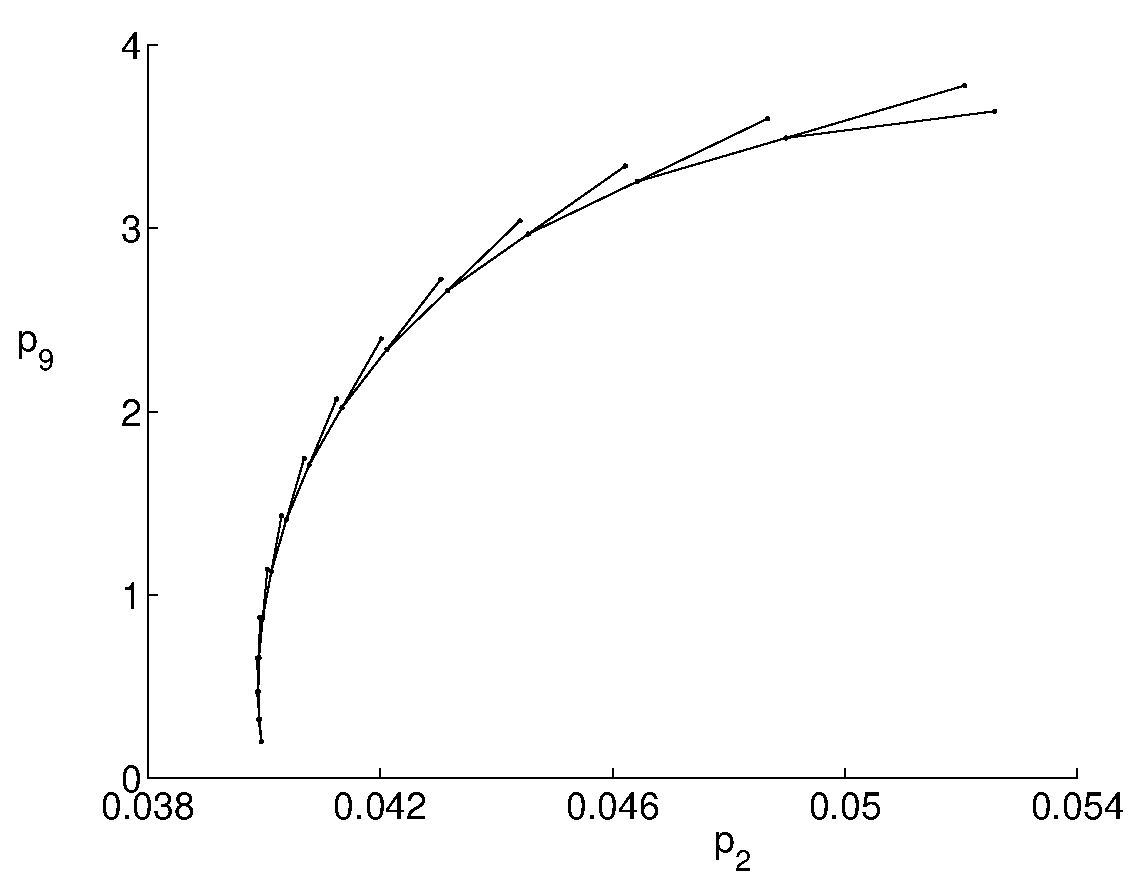
\includegraphics{fig/sdd3.eps}}
\end{center}
\caption{\small\label{br_hopf} Predictions and corrections
in the $(p_2,p_9)$-plane after computation of a branch of Hopf-like 
bifurcations.}
\end{figure}

We use the first Hopf-like point in the $\parm{branch2}$ 
to construct a small amplitude ($1e-1$)
periodic solution on an equidistant mesh of
$15$ intervals with piecewise polynomial degree $3$.
{\small\begin{verbatim}
>> hopf=branch2.point(1);
>> intervals=15;
>> degree=3;
>> [psol,stepcond]=p_topsol(hopf,1e-1,degree,intervals);
\end{verbatim}}
The steplength condition returned ensures the branch switch from the
Hopf to the periodic solution as it avoids convergence of  
the amplitude 
to zero during corrections. Due to the presence of the
steplength condition we also need to
free one parameter, here $\tau_1$ (parameter 10).
{\small\begin{verbatim}
>> method=df_mthod('psol');
>> [psol,success]=p_correc(psol,10,stepcond,method.point)
psol = kind: 'psol'
  parameter: [1x11 double]
       mesh: [1x46 double]
     degree: 3
    profile: [5x46 double]
     period: 11.4306 
success = 1
\end{verbatim}}
The result, along with a degenerate periodic solution with amplitude
zero, is used to start on the emanating branch of periodic solutions,
see figure \ref{br_ps_sd1} (left). We use adaptive mesh selection.
Note that in the case of sd-DDEs, $\parm{min\_bound}$
for a constant delay being a continuation parameter
should be defined in the same way as for other continuation parameters.
{\small\begin{verbatim}
>> branch3=df_brnch(10,'psol');
>> branch3.parameter.min_bound(1,:)=[10 0];
>> branch3.parameter.max_bound(1,:)=[10 10];
>> branch3.parameter.max_step(1,:)=[10 0.01];
>> deg_psol=p_topsol(first_hopf,0,degree,intervals);
>> branch3.point=deg_psol;
>> branch3.point(2)=psol;
>> figure(4); clf;
>> [branch3,s,f,r]=br_contn(branch3,10);
>> point=branch3.point(end);
>> p_ampl=max(point.profile(1,:))-min(point.profile(1,:));
>> plot(point.parameter(10),p_ampl,'o');
\end{verbatim}}
\begin{figure}[h]
\begin{center}
\resizebox{6cm}{!}{\includegraphics{fig/sdd4.eps}}
\resizebox{6cm}{!}{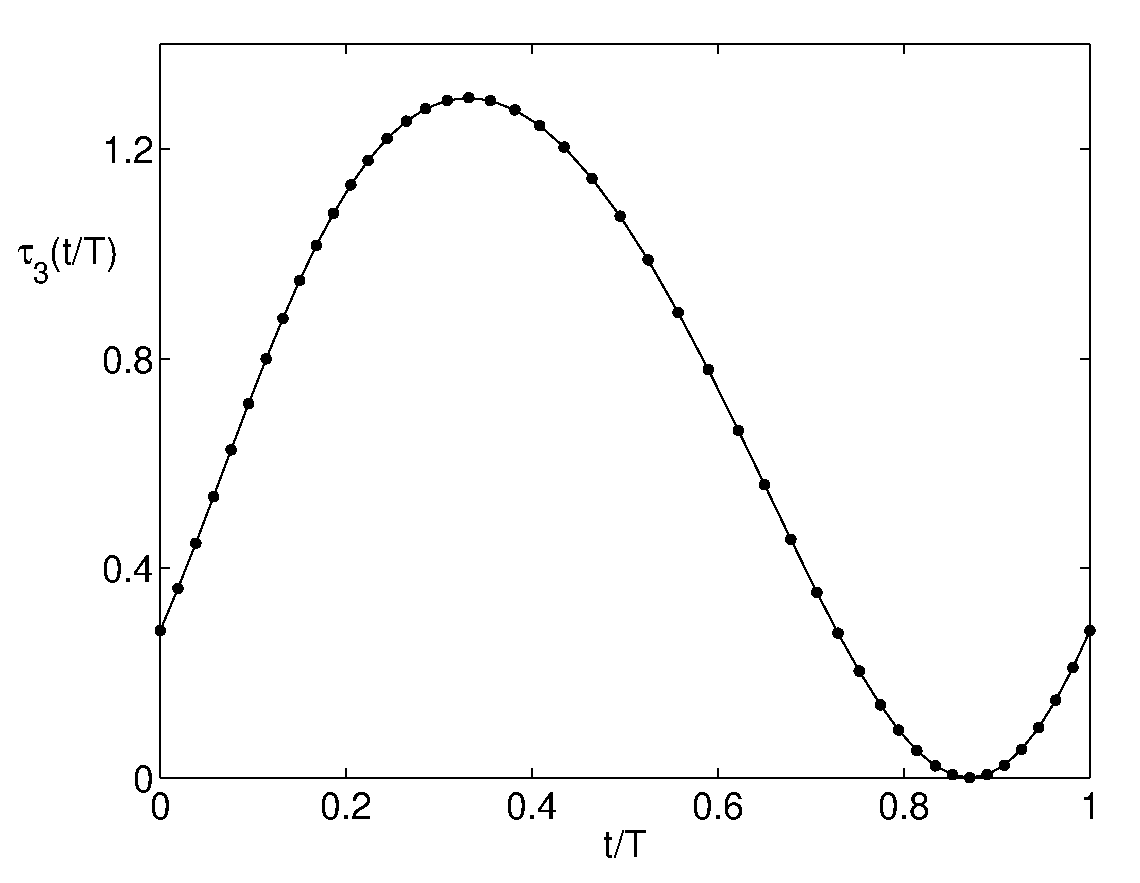
\includegraphics{fig/sdd5.eps}}
\end{center}
\caption{\small\label{br_ps_sd1}Left: Branch of periodic solutions emanating
from a Hopf-like point. $\circ$ - the last computed point in the branch
(corresponding to $\tau_3(\parm{tz})=0$). Right: $\tau_3(t/T)$ at 
the last computed point. Dots indicate representation points
of the mesh used.}
\end{figure}
As in the case of computing $\parm{branch1}$, we have a warning,
{\small\begin{verbatim}
BR_CONTN warning: delay number_3 becomes negative.
\end{verbatim}}
\noindent
indicating that the delay function $\tau_3(t)$ became negative
at some point(s) on the period interval of the computed solution
during continuation of the branch.
The periodic solution with $\tau_3(t)$ negative is not accepted as the 
branch point.
Instead, the following algorithm is executed. First, using the solution
with $\tau_3(t)$ negative and a mesh refinement, a time point 
$\parm{tz}$ is computed at which $\tau_3(t)$ reaches its minimum.
Then, a periodic solution is computed under the conditions,
\begin{equation}\label{tz_cond}
\tau_3(\parm{tz})=0, \: \: \: \: \: {\d}\tau_3(\parm{tz})/{\d}t=0.
\end{equation}
We compute and plot the delay $\tau_3(t)$ on the mesh of representation points
at the last accepted point in the
branch, see figure~\ref{br_ps_sd1} (right).
{\small\begin{verbatim} 
>> tau_eva=p_tau(branch3.point(end),3);
>> figure(5); clf;
>> plot(branch3.point(end).mesh,tau_eva);
>> hold;
>> plot(branch3.point(end).mesh,tau_eva,'.');
>> min(tau_eva) 
ans = 9.6557e-04
\end{verbatim}}
\noindent
The last result says that $\tau_3(t)$  has its minimal value 
at a point between two representation points.

Now we use the last Hopf-like point in the $\parm{branch2}$ 
to compute a branch of periodic solutions as a function of 
the parameter $p_1$, see figure~\ref{br_ps_sd2} (left).
{\small\begin{verbatim}
>> hopf=branch2.point(end);
>> intervals=15;
>> degree=3;
>> [psol,stepcond]=p_topsol(hopf,1e-1,degree,intervals);
>> method=df_mthod('psol');
>> [psol,success]=p_correc(psol,1,stepcond,method.point)
psol = kind: 'psol'
  parameter: [1x11 double]
       mesh: [1x46 double]
     degree: 3
    profile: [5x46 double]
     period: 12.6610
success = 1
\end{verbatim}}

{\small\begin{verbatim}
>> branch4=df_brnch(1,'psol');
>> branch4.parameter.min_bound(1,:)=[1 0];
>> branch4.parameter.max_bound(1,:)=[1 10];
>> branch4.parameter.max_step(1,:)=[1 0.01];
>> deg_psol=p_topsol(hopf,0,degree,intervals);
>> branch4.point=deg_psol;
>> branch4.point(2)=psol;
>> figure(5); clf;
>> [branch4,s,f,r]=br_contn(branch4,10);
>> point=branch4.point(end);
>> p_ampl=max(point.profile(1,:))-min(point.profile(1,:));
>> plot(point.parameter(1),p_ampl,'o');
\end{verbatim}}
\begin{figure}[h]
\begin{center}
\resizebox{6cm}{!}{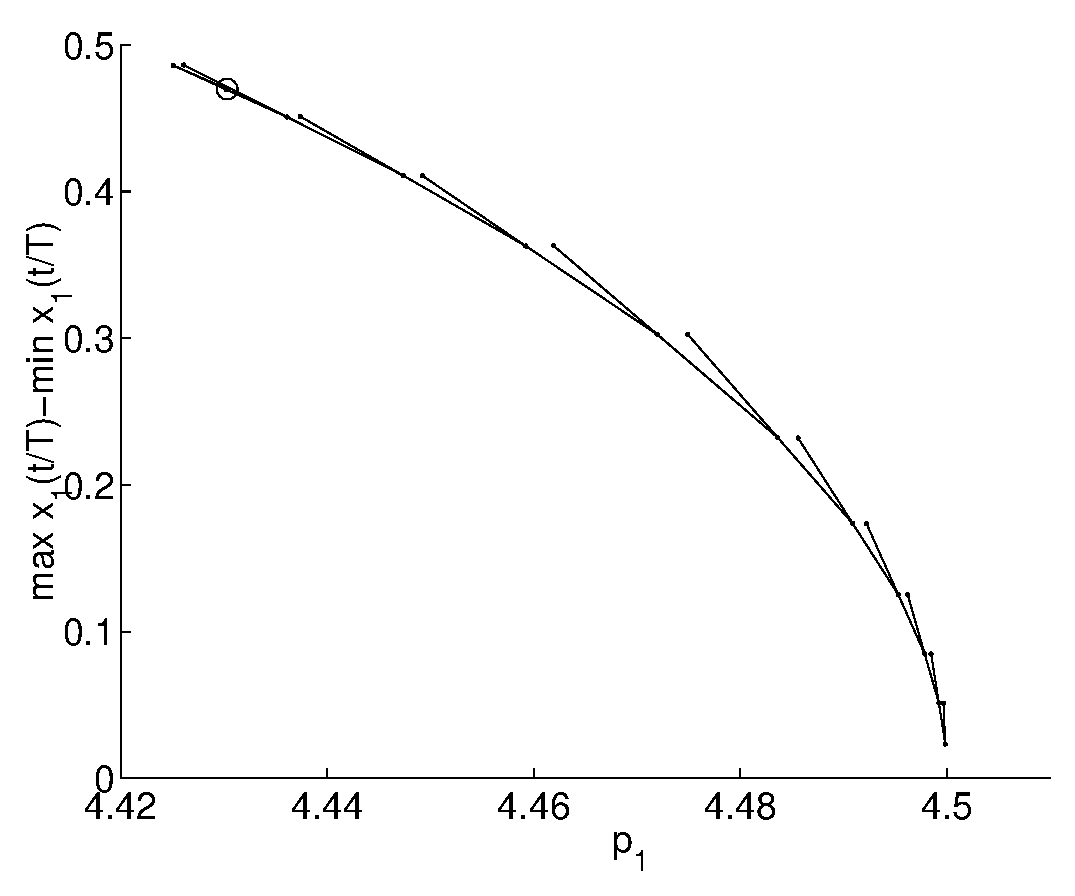
\includegraphics{fig/sdd6.eps}}
\resizebox{6cm}{!}{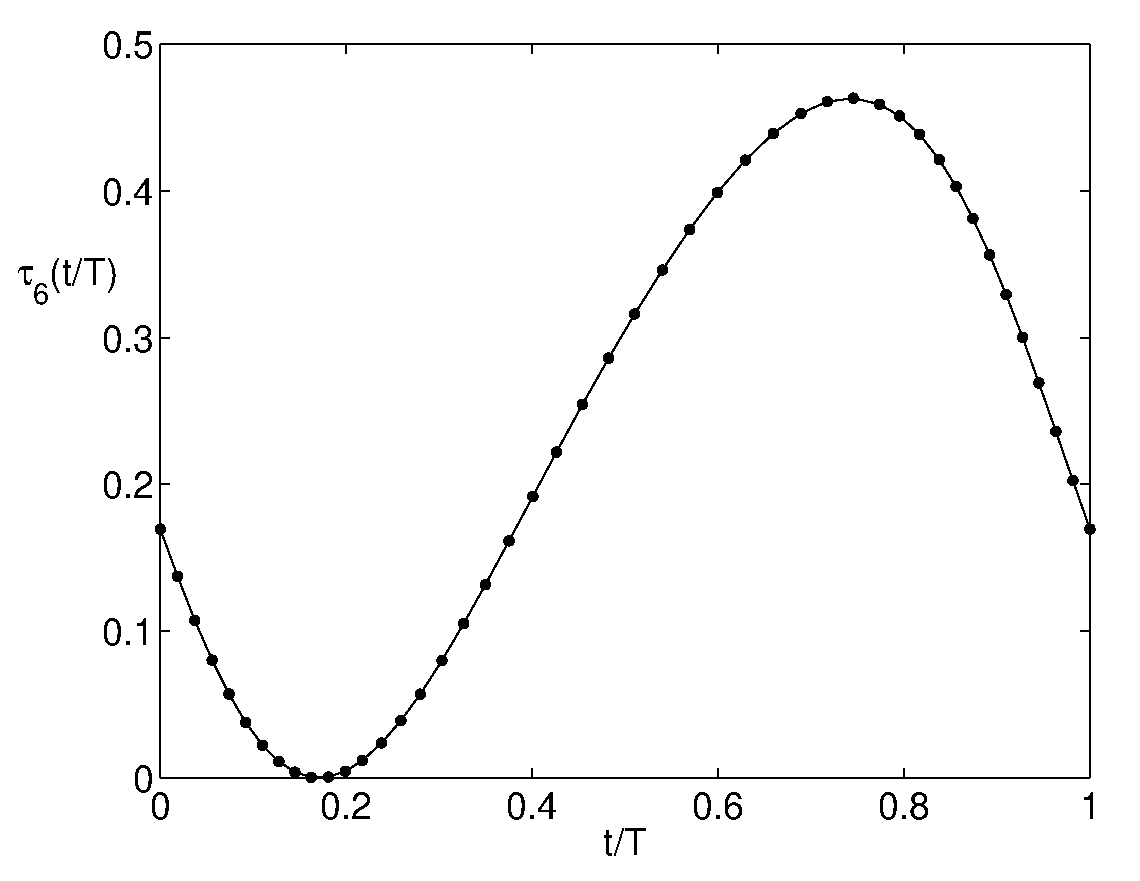
\includegraphics{fig/sdd7.eps}}
\end{center}
\caption{\small\label{br_ps_sd2}Left: Branch of periodic solutions emanating
from a Hopf-like point. $\circ$ - the last computed point in the branch
(corresponding to $\tau_6(\parm{tz})=0$). Right: $\tau_6(t/T)$ at 
the last computed point. Dots indicate representation points
of the mesh used.}
\end{figure}
We again have a warning,
{\small\begin{verbatim}
BR_CONTN warning: delay number_6 becomes negative.
\end{verbatim}}
We plot the delay $\tau_6(t)$ (recall that $\tau_6(t)=x_5(t)$)
on the mesh of representation points at the last accepted point 
in the branch, see figure~\ref{br_ps_sd2} (right).
{\small\begin{verbatim}
>> psol=branch4.point(end); 
>> figure(7); clf;
>> plot(psol.mesh,psol.profile(5,:));
>> hold;
>> plot(psol.mesh,psol.profile(5,:),'.');
>> min(psol.profile(5,:)) 
ans = -5.8556e-31
\end{verbatim}}
The minimal value of the delay $\tau_6$ is a negative value. 
The stability of the corresponding solution is computed if this 
value is larger 
than the one defined in $\parm{method.stability.delay\_accuracy}$
(see table~\ref{meth_stab_struct}).
The result of computing and plotting stability (Floquet multipliers) 
of this periodic solution is shown in 
figure~\ref{sd_dde_mu}. The solution is unstable.
{\small\begin{verbatim}
>> psol.stability=p_stabil(psol,method.stability);
>> psol.stability.mu
ans = 1.3253
      1.0000
      0.0959
figure(8); clf;
p_splot(psol);
axis image;
\end{verbatim}}
\begin{figure}[h]
\begin{center}
\resizebox{6cm}{!}{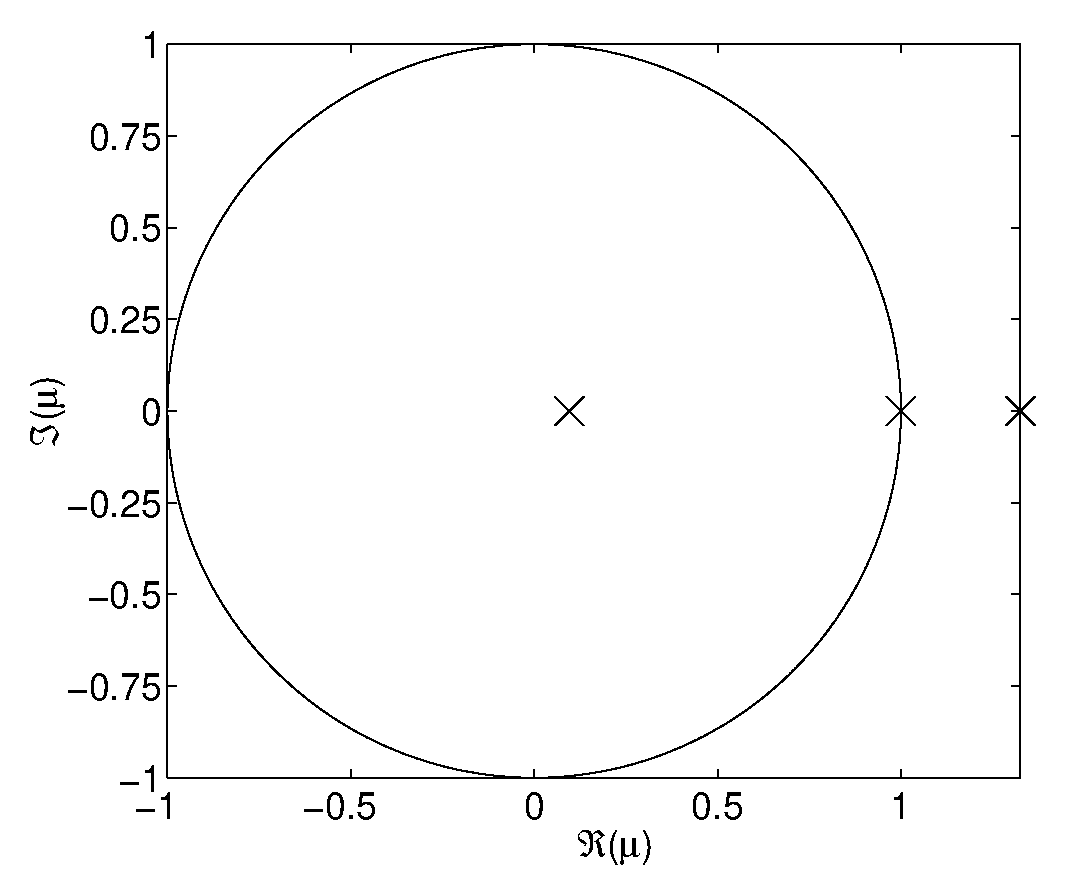
\includegraphics{fig/sdd8.eps}}
\end{center}
\caption{\small\label{sd_dde_mu}Floquet multipliers for the periodic 
solution at the last computed point in the $\parm{branch4}$.} 
\end{figure}


\subsection{Connecting orbits demo: analysis of branches of homoclinic orbits}\label{demo3}
This demo describes how to use \DDEBIFCODE\ to perform a bifurcation analysis on equations
with several constant delays which exhibit connecting orbits.  
System definitions files  (see section \ref{sys_def1}) can be
found in the directory \verb$HOM_DEMO$.  The commands used in this demo are listed in the file 
\file{hom\_demo.m}.
As mentioned at the end of the first demo, one can compute connecting
orbits using a direct method, when the delays are not state-dependent 
In order to show the use of this method,
we will now investigate a model of neural activity, described in \cite{zapp}.

\parbox{10cm}{
\begin{eqnarray*}
\dot{x}_{1}(t)&=&-x_{1}(t)+q_{11}\frac{1}{1+e^{-4x_{1}(t-\tau)}}-q_{12}x_2(t-\tau) +e_1\\
\dot{x}_{2}(t)&=&-x_2(t)+q_{21}\frac{1}{1+e^{-4x_{1}(t-\tau)}}+e_2
\end{eqnarray*}
}
\hfill \parbox{1cm}{\begin{eqnarray}\label{z}\end{eqnarray}}

The focus will be on the analysis of the homoclinic orbits in 
this system.  Therefore, we will not repeat the standard bifurcation analysis.
The reader is advised to run through section \ref{ride-through} to become more
familiar with the analysis.  For the purpose of this demo,
 we start at a point where branches of Hopf points and fold points have 
already been computed. Figure \ref{demo3-1} shows branches of 
fold and Hopf points, plotted with respect to the two free parameters of the 
system, $q_{12}$ and $e_1$.  To obtain this figure, we first load the 
precomputed (and saved) branches from the file \file{hcl\_demo.mat}.  
We choose to
plot the branches with respect to their default measure.
{\small\begin{verbatim}
>> sys_init;
>> load hom_demo;
>> figure(1);
>> [xm,ym]=df_measr(0,fold_branch);
>> br_plot(fold_branch,xm,ym,':');
>> axis([1.28 1.62 -1.36 -1.24]);
>> hold on;
>> br_plot(hopf1_branch,xm,ym,'-.');
>> br_plot(hopf2_branch,xm,ym,'-.');
\end{verbatim}}
\begin{figure}[ht]
\begin{center}
\resizebox{6cm}{!}{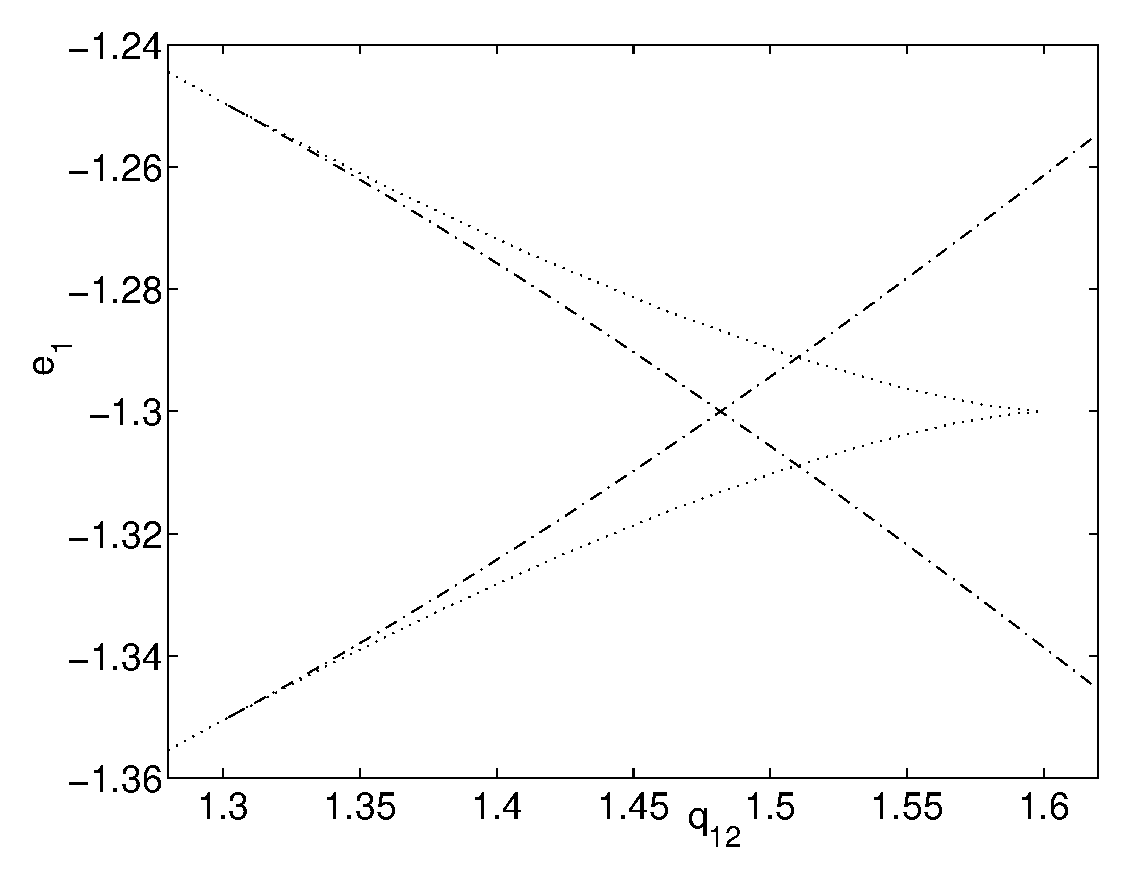
\includegraphics{fig/demo3-1.eps}}
\caption{\small\label{demo3-1}Branches of fold ('$\cdots$') and 
Hopf ('$-\cdot$') points of system (\ref{z}).}
\end{center}
\end{figure}

We then select a Hopf point somewhere on the lower branch, 
and start the branch of
periodic solutions that emanates from it.  For this purpose, we create a
branch of periodic solutions with two points. We choose to plot the 
period versus the free
parameter while continuing, in order to visualize 
the approaching of the homoclinic orbit, see 
Figure \ref{demo3-2}.
{\small\begin{verbatim}
>> hopf=hopf1_branch.point(27);
>> [psol,stp]=p_topsol(hopf,1e-2,3,27)
psol = kind:'psol'
  parameter: [2.6000e+00 1.3428e+00 1 -1.3398e+00 -5.0000e-01 1]
     degree: 3
    profile: [2x82 double]
     period: 5.5271e+01
 stp = kind: 'psol'
  parameter: [0 0 0 0 0 0]
       mesh: [1x82 double]
     degree: 3
    profile: [2x82 double]
     period: 0

>> mpsol=df_mthod('psol');
>> [psol,s]=p_correc(psol,4,stp,mpsol.point);
>> psol_branch=df_brnch(4,'psol');
>> psol_branch.point=psol;
>> [psol,stp]=p_topsol(hopf,2e-2,3,27);
>> [psol,s]=p_correc(psol,4,stp,mpsol.point);
>> psol_branch.point(2)=psol;
>> figure(2);clf;
>> [xm,ym]=df_measr(0,psol_branch);
>> ym.field='period';
>> ym.col=1;
>> ym.row=1;
>> psol_branch.method.continuation.plot_measure.x=xm;
>> psol_branch.method.continuation.plot_measure.y=ym;
>> [psol_branch,s,r,f]=br_contn(psol_branch,20);
\end{verbatim}}

\begin{figure}[ht]
\begin{center}
\resizebox{6cm}{!}{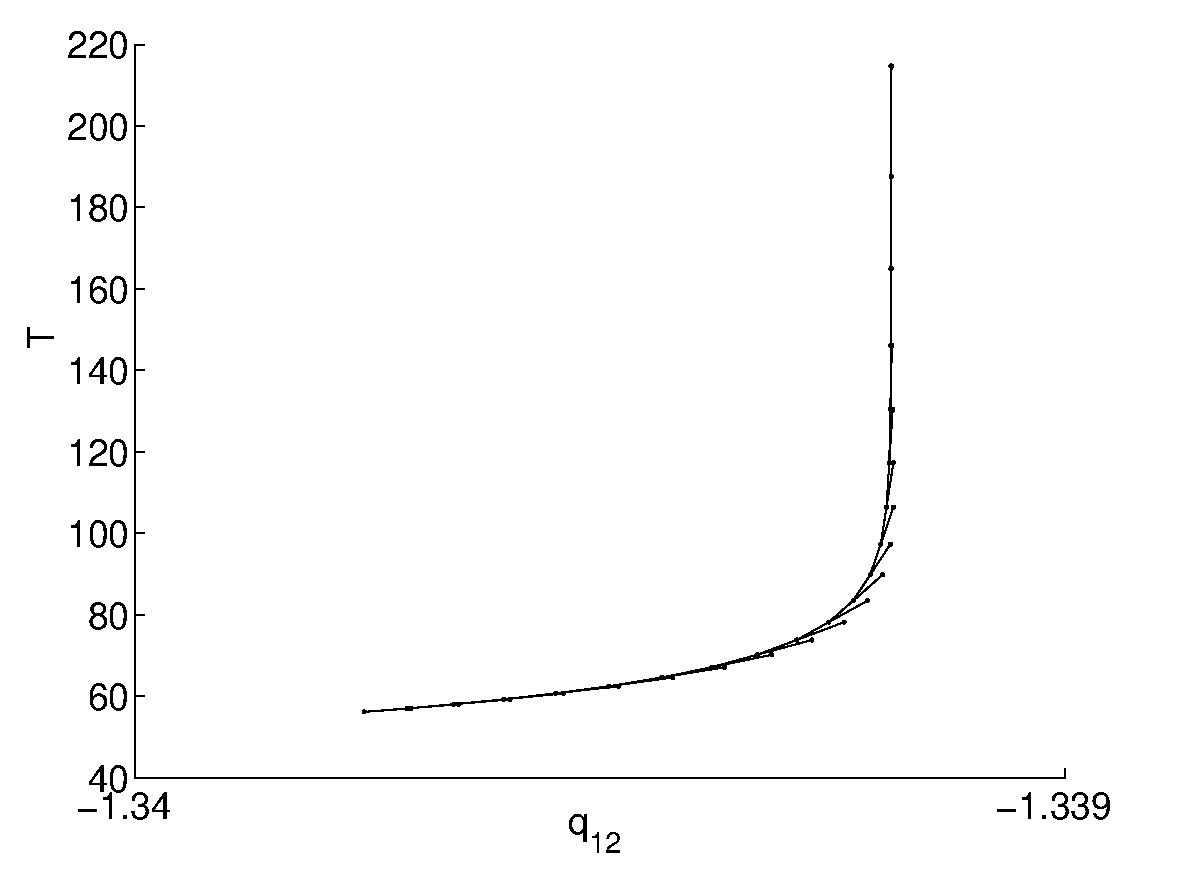
\includegraphics{fig/demo3-2.eps}}
\caption{\small\label{demo3-2}Period of the periodic orbits of system (\ref{z}), as a
 function of the parameter $q_{12}$.}
\end{center}
\end{figure}

It is shown in Figure \ref{demo3-3} that the last point of this branch of periodic solutions is close to a homoclinic orbit.
{\small\begin{verbatim}
>> figure(3);clf;
>> psol=psol_branch.point(end)
psol =   kind: 'psol'
    parameter: [2.6000e+00 1.3428e+00 1 -1.3392e+00 -5.0000e-01 1]
         mesh: [1x82 double]
       degree: 3
      profile: [2x82 double]
       period: 2.1469e+02

>> p_pplot(psol);
\end{verbatim}}

\begin{figure}[ht]
\begin{center}
\resizebox{6cm}{!}{\includegraphics{fig/demo3-3.eps}}
\caption{\small\label{demo3-3}Profile of a periodic solution with large period of
system (\ref{z}), close
to a homoclinic orbit}
\end{center}
\end{figure}

We convert this point to a point of homoclinic type. This yields an 
(uncorrected) initial homoclinic profile.  Note that the steady state is also 
uncorrected.
{\small\begin{verbatim}
>> hcli=p_tohcli(psol)
hcli =   kind: 'hcli'
    parameter: [2.6000e+00 1.3428e+00 1 -1.3392e+00 -5.0000e-01 1]
         mesh: [1x79 double]
       degree: 3
      profile: [2x79 double]
       period: 1.8216e+02
           x1: [2x1 double]
           x2: [2x1 double]
     lambda_v: 1.6906e-01
     lambda_w: 1.6906e-01
            v: [2x1 double]
            w: [2x1 double]
        alpha: -1
      epsilon: 5.2583e-06
\end{verbatim}}
We correct this point, after remeshing it on an adaptive mesh
with 50 intervals.  We plot this point before and after correction, 
see Figure \ref{demo3-4+5}.
{\small\begin{verbatim}
>> figure(4);clf;
>> p_pplot(hcli);
>> mhcli=df_mthod('hcli');
>> [hcli,s]=p_correc(hcli,4,[],mhcli.point);
>> hcli=p_remesh(hcli,3,50);
>> [hcli,s]=p_correc(hcli,4,[],mhcli.point)
hcli =   kind: 'hcli'
    parameter: [2.6000e+00 1.3428e+00 1 -1.3392e+00 -5.0000e-01 1]
         mesh: [1x151 double]
       degree: 3
      profile: [2x151 double]
       period: 1.8806e+02
           x1: [2x1 double]
           x2: [2x1 double]
     lambda_v: 1.6905e-01
     lambda_w: 1.6905e-01
            v: [2x1 double]
            w: [2x1 double]
        alpha: -1
      epsilon: 5.2583e-06
s = 1
>> figure(5);clf;
>> p_pplot(hcli);
\end{verbatim}
}
\begin{figure}[ht]
\begin{center}
\subfigure{\resizebox{6cm}{!}{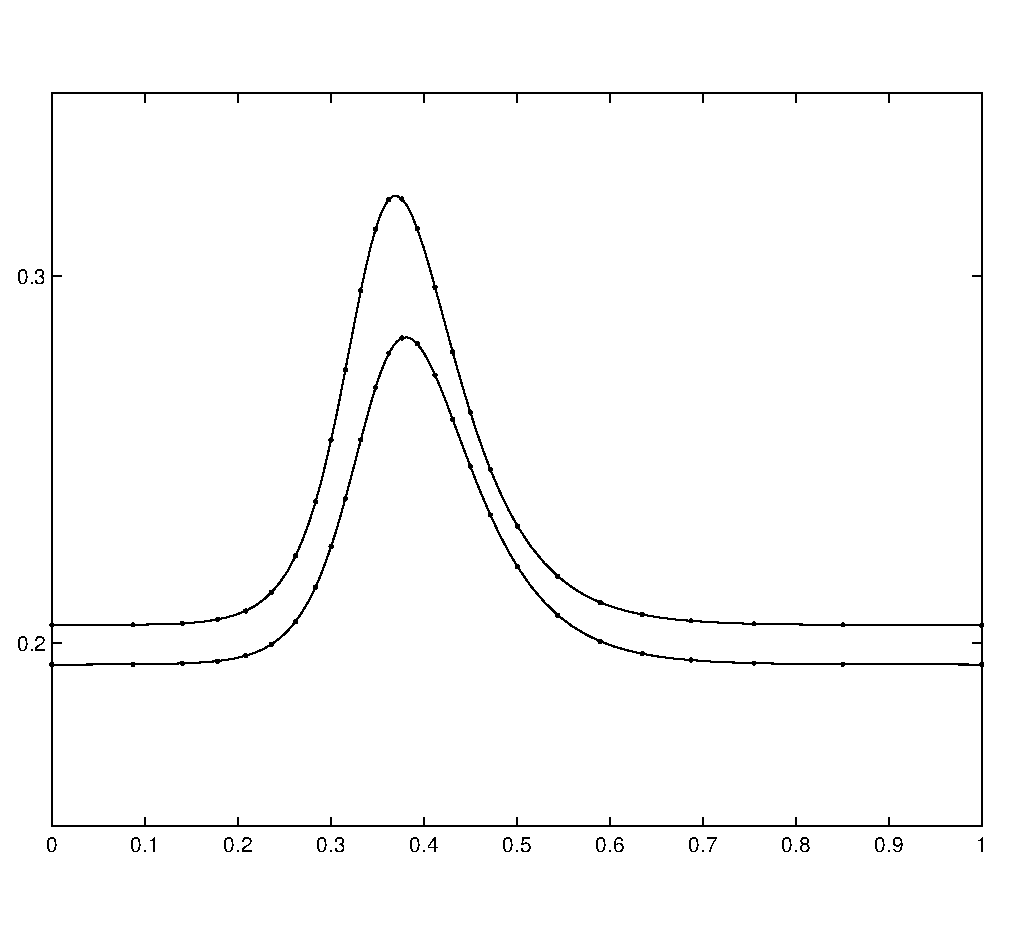
\includegraphics{fig/demo3-4.eps}}}
\subfigure{\resizebox{6cm}{!}{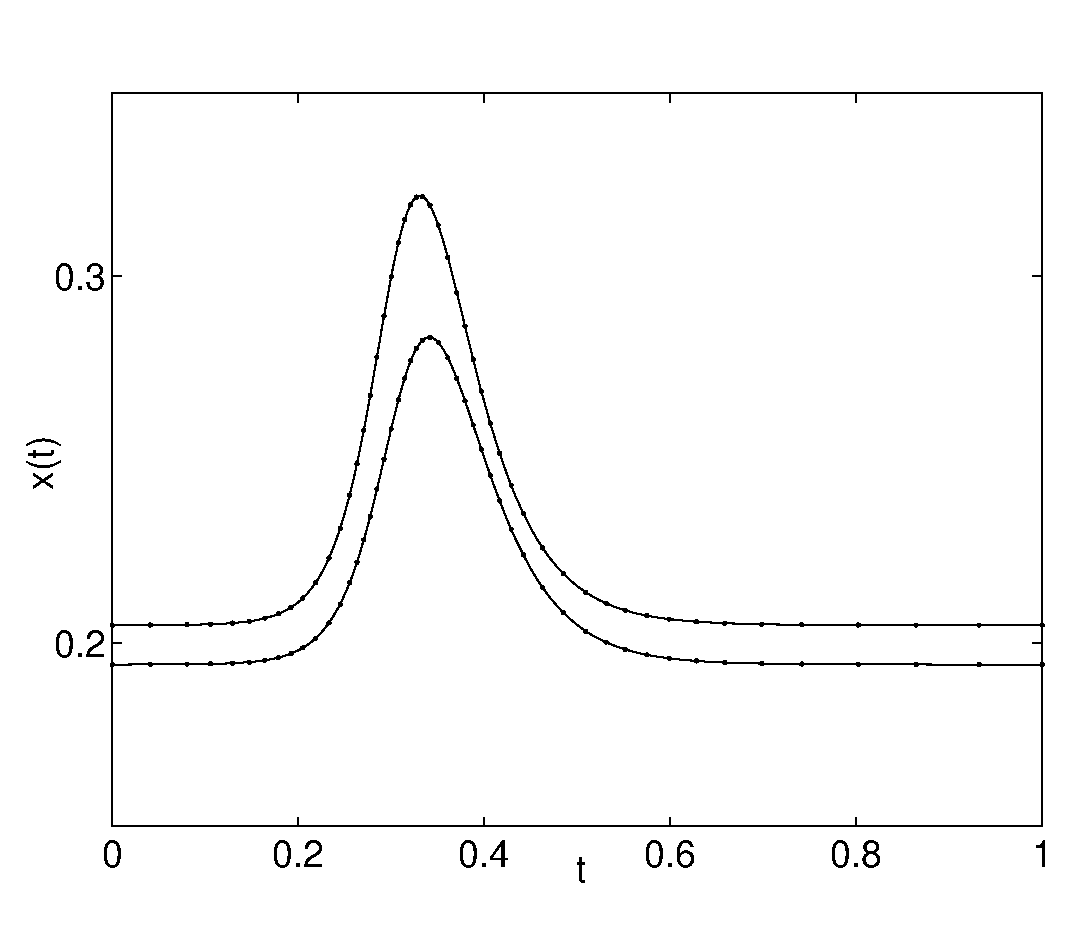
\includegraphics{fig/demo3-5.eps}}}
\caption{\small Left: initial profile (before correction) of a homoclinic orbit of 
system (\ref{z}). Right: remeshed and corrected profile of the same homoclinic 
orbit. \label{demo3-4+5}} 
\end{center}
\end{figure}

We slightly change parameter values of this homoclinic orbit, and compute
a second homoclinic orbit.  With these two homoclinic solutions, 
we then
create a branch, which is continued in two free parameters ($e_1$ 
and $q_{12}$).

{\small\begin{verbatim}
>> hcli_br=df_brnch([2 4],'hcli');
>> hcli_br.point=hcli;
>> hcli.parameter(2)=hcli.parameter(2)+6e-3;
>> [hcli,s]=p_correc(hcli,4,[],mhcli.point);
>> hcli_br.point(2)=hcli;
>> figure(1);
>> [hcli_br,s,r,f]=br_contn(hcli_br,85)
hcli_br = method: [1x1 struct]
       parameter: [1x1 struct]
           point: [1x71 struct]
s = 70
r = 16
f = 0
>> hcli_br=br_rvers(hcli_br);
>> [hcli_br,s,r,f]=br_contn(hcli_br,10)
hcli_br = method: [1x1 struct]
       parameter: [1x1 struct]
           point: [1x81 struct]
s = 11
r = 0
f = 0 
\end{verbatim}}
We do exactly the same for the second branch of Hopf points.  Since 
the bifurcation diagram of this system is completely symmetric, 
we also approach 
homoclinic orbits when we jump onto the branches of periodic solutions 
emanating
from those Hopf points.  The commands are the same as in the above case,
so we simply list them, without further explanation.  We also do not
plot the branch of periodic solutions while continuing.
{\small\begin{verbatim}
>> hopf=hopf2_branch.point(27);
>> [psol,stp]=p_topsol(hopf,1e-2,3,27);
>> mpsol=df_mthod('psol');
>> [psol,s]=p_correc(psol,4,stp,mpsol.point);
>> psol_branch=df_brnch(4,'psol');
>> psol_branch.point=psol;
>> [psol,stp]=p_topsol(hopf,2e-2,3,27);
>> [psol,s]=p_correc(psol,4,stp,mpsol.point);
>> psol_branch.point(2)=psol;
>> psol_branch.method.continuation.plot=0;
>> psol_branch.method.continuation.plot_progress=0;
>> [psol_branch,s,r,f]=br_contn(psol_branch,20);

>> psol=psol_branch.point(end-1);
>> hcli=p_tohcli(psol);
>> mhcli=df_mthod('hcli');
>> [hcli,s]=p_correc(hcli,4,[],mhcli.point);
>> hcli=p_remesh(hcli,3,50);
>> [hcli,s]=p_correc(hcli,4,[],mhcli.point);

>> hcli2_br=df_brnch([2 4],'hcli');
>> hcli2_br.point=hcli;
>> hcli.parameter(4)=hcli.parameter(4)+1e-3;
>> [hcli,s]=p_correc(hcli,2,[],mhcli.point);
>> hcli2_br.point(2)=hcli;
>> figure(1);
>> hcli2_br=br_rvers(hcli2_br);
>> [hcli2_br,s,r,f]=br_contn(hcli2_br,85)
hcli2_br = method: [1x1 struct]
        parameter: [1x1 struct]
            point: [1x70 struct]
s = 69
r = 17
f = 0

>> hcli2_br=br_rvers(hcli2_br);
>> [hcli2_br,s,r,f]=br_contn(hcli2_br,10)
hcli2_br = method: [1x1 struct]
        parameter: [1x1 struct]
            point: [1x80 struct]
s = 11
r = 0
f = 0
\end{verbatim}}

The resulting branches of homoclinic solutions are shown in 
Figure~\ref{demo3-1b}.
\begin{figure}[ht]
\begin{center}
\resizebox{6cm}{!}{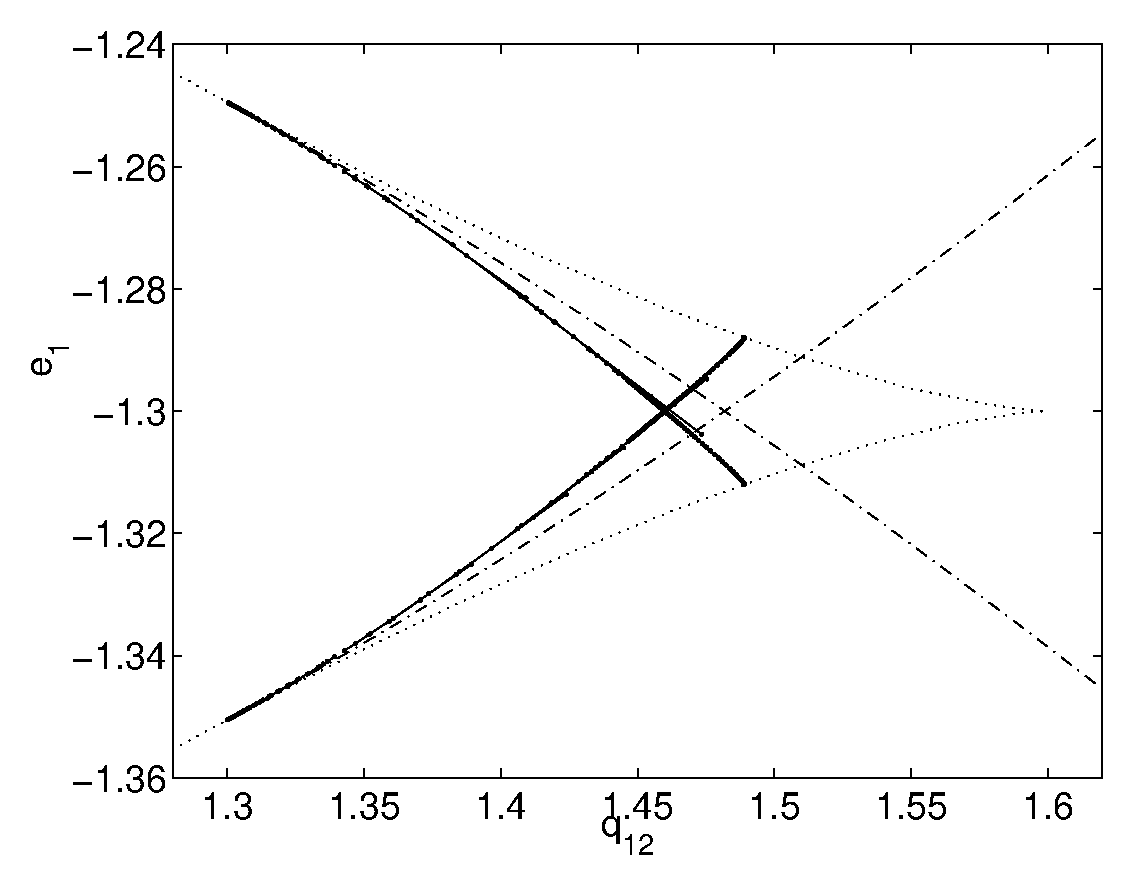
\includegraphics{fig/demo3-1b.eps}}
\caption{\small\label{demo3-1b}Bifurcation diagram of system (\ref{z}), like 
in Figure \ref{demo3-1}, now also showing two branches of homoclinic 
solutions (predictions and corrections).}
\end{center}
\end{figure}
They both end at the branch of fold points, as the stability of the 
steady state
changes at this point.  At $e_{1}=-1.3$, a double homoclinic orbit exists. 
This is easily shown as follows. First, we look for the point 
on the branch where $e_{1}=-1.3$.  
{\small\begin{verbatim}
>> figure(6);
>> [xm,ym]=df_measr(0,hcli_br);
>> br_plot(hcli2_br,[],ym);
>> hold on;
>> plot([0 110],[-1.3 -1.3],'r-.');
>> axis([22 40 -1.304 -1.294]);
\end{verbatim}}
As Figure \ref{demo3-6} shows, this is the 30th point along the lower branch 
and the 26th along the upper branch.
\begin{figure}[ht]
\begin{center}
\resizebox{6cm}{!}{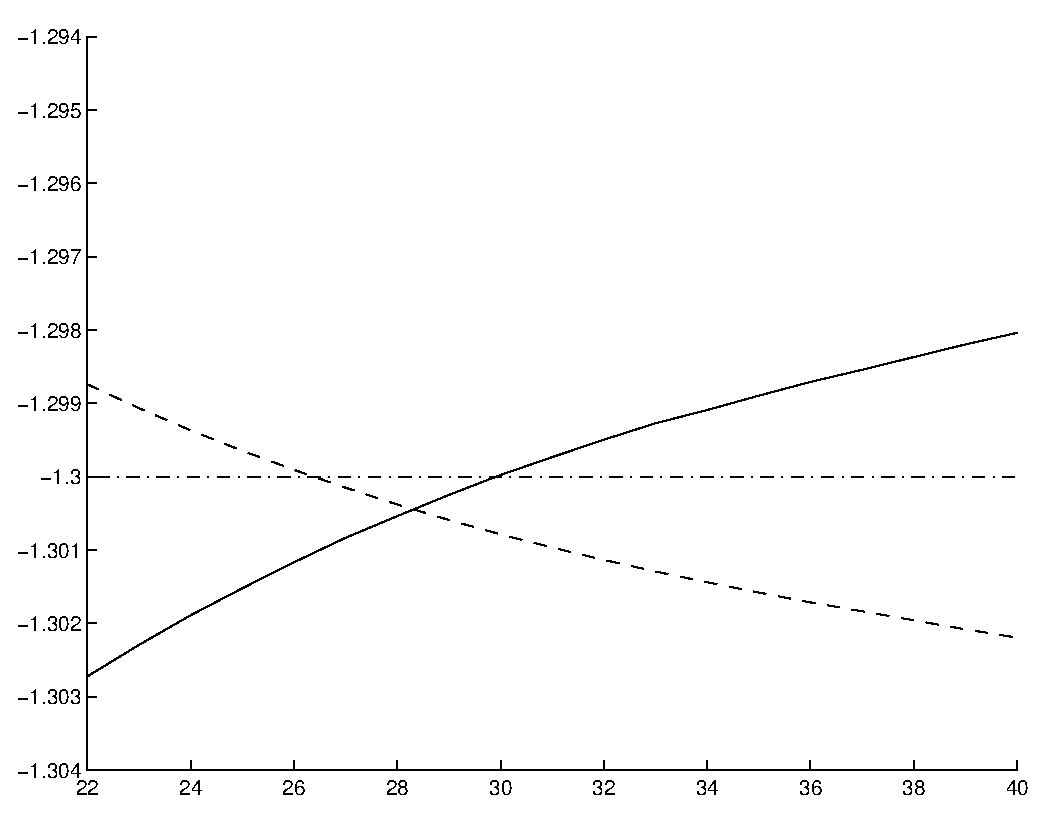
\includegraphics{fig/demo3-6.eps}}
\caption{\small\label{demo3-6}Evolution of parameter $e_1$ vs. point number
along the lower (solid) and upper (dashed) branches of homoclinic orbits.}
\end{center}
\end{figure}
 The double homoclinic orbit
is plotted in Figure \ref{demo3-7}.
{\small\begin{verbatim}
>> figure(7);
>> plot(hcli2_br.point(30).profile(1,:),hcli2_br.point(30).profile(2,:));
>> hold on;
>> plot(hcli_br.point(26).profile(1,:),hcli_br.point(26).profile(2,:));
\end{verbatim}}
\begin{figure}[ht]
\begin{center}
\resizebox{6cm}{!}{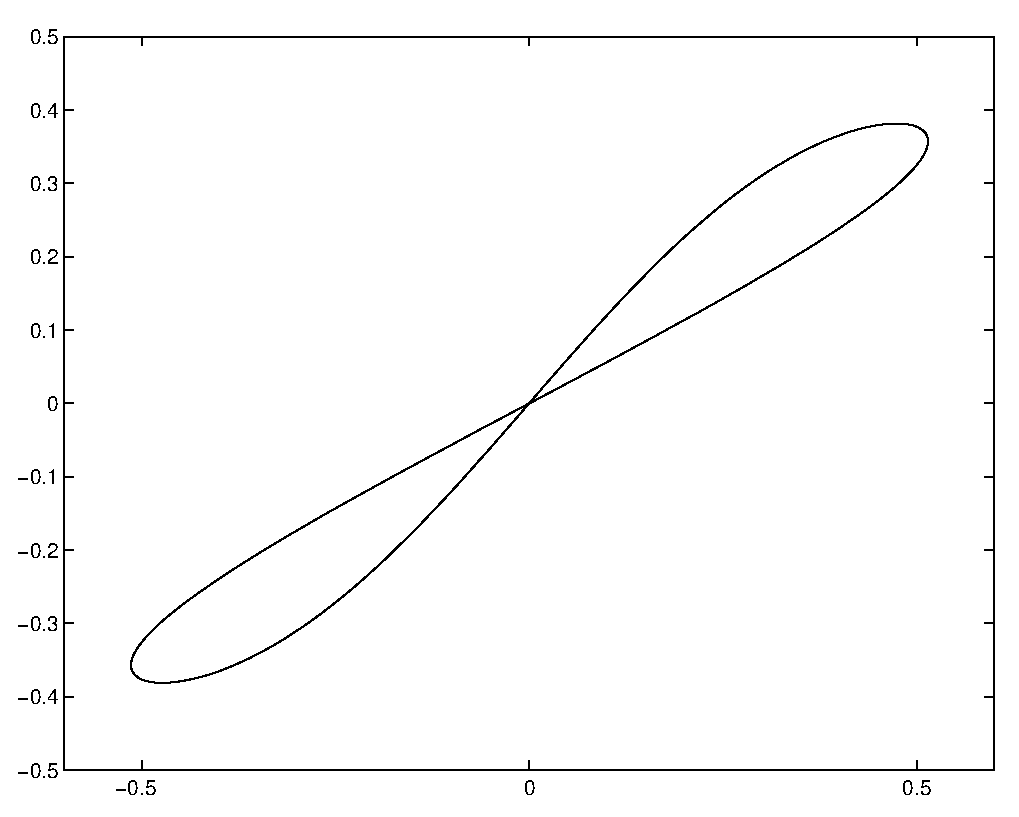
\includegraphics{fig/demo3-7.eps}}
\caption{\small\label{demo3-7}Phase portrait of the double homoclinic orbit of system
(\ref{z}) for 
$e_{1}=-1.3$.}
\end{center}
\end{figure}
Both branches of homoclinic orbits emanate from a Takens-Bogdanov bifurcation.
 As the amplitude of the homoclinic orbits along the branch goes to zero, the 
steady state approaches a Takens-Bogdanov-point. To illustrate this, Figure
\ref{demo3-8} shows the stability information of the last computed point 
on the branch. We see two small eigenvalues, but we are still at some distance
from the Takens-Bogdanov point.
\begin{figure}
\begin{center}
\resizebox{6cm}{!}{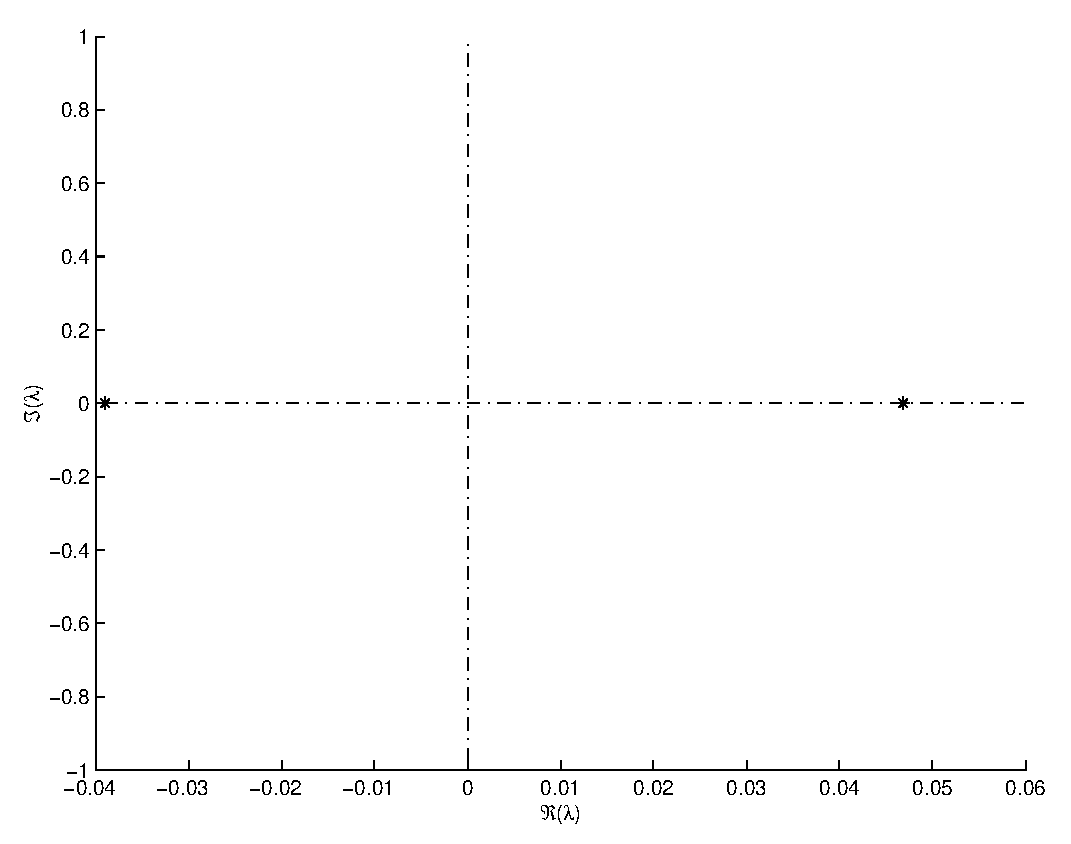
\includegraphics{fig/demo3-8.eps}}
\caption{\small Dominant eigenvalues of the saddle of the last point on the first branch
of homoclinic orbits,
near a Takens-Bogdanov bifurcation.\label{demo3-8}}
\end{center}
\end{figure}
{\small\begin{verbatim}
>> figure(8);
>> stst=p_tostst(hcli_br.point(end));
>> stst=stst(1);
>> mstst=df_mthod('stst');
>> stst.stability=p_stabil(stst,mstst.stability);
>> p_splot(stst);
\end{verbatim}}

In order to be able to continue the branch of homoclinic orbits closer to
this Takens-Bogdanov point, we form a 
new branch, starting from the last point (with the profile remeshed on a
finer mesh), and using a much smaller step size.  If we would
 not do this, the 
steplength selection strategy (see section \ref{continuation}) will take 
too large steps, resulting in a turnaround and a backward 
computation of the same branch.
We continue this new branch.  During this continuation, it is possible
that Matlab displays a warning concerning the near-singular character of the
system being solved.  This is an indication that we are close to the Takens-Bogdanov singularity.  We then look again to the dominant eigenvalues of the 
last point, see Figure \ref{demo3-9}.  
  It is clear that this point is much closer to the Takens-Bogdanov
point.
{\small\begin{verbatim}
>> hcli=hcli_br.point(end);
>> hcli=p_remesh(hcli,3,70);
>> [hcli,s]=p_correc(hcli,4,[],mhcli.point);
>> to_tb_branch=df_brnch([2 4],'hcli');
>> to_tb_branch.point=hcli;
>> hcli.parameter(2)=hcli.parameter(2)-1e-4;
>> hcli=p_remesh(hcli,3,70);
>> [hcli,s]=p_correc(hcli,4,[],mhcli.point);
>> to_tb_branch.point(2)=hcli;
>> to_tb_branch.method.continuation.plot=0;
>> to_tb_branch.method.continuation.plot_progress=0;
>> [to_tb_branch,s,r,f]=br_contn(to_tb_branch,40);

>> figure(9);
>> stst=p_tostst(to_tb_branch.point(end));
>> stst=stst(1);
>> mstst=df_mthod('stst');
>> stst.stability=p_stabil(stst,mstst.stability);
>> p_splot(stst);
\end{verbatim}
}

\begin{figure}
\begin{center}
\resizebox{6cm}{!}{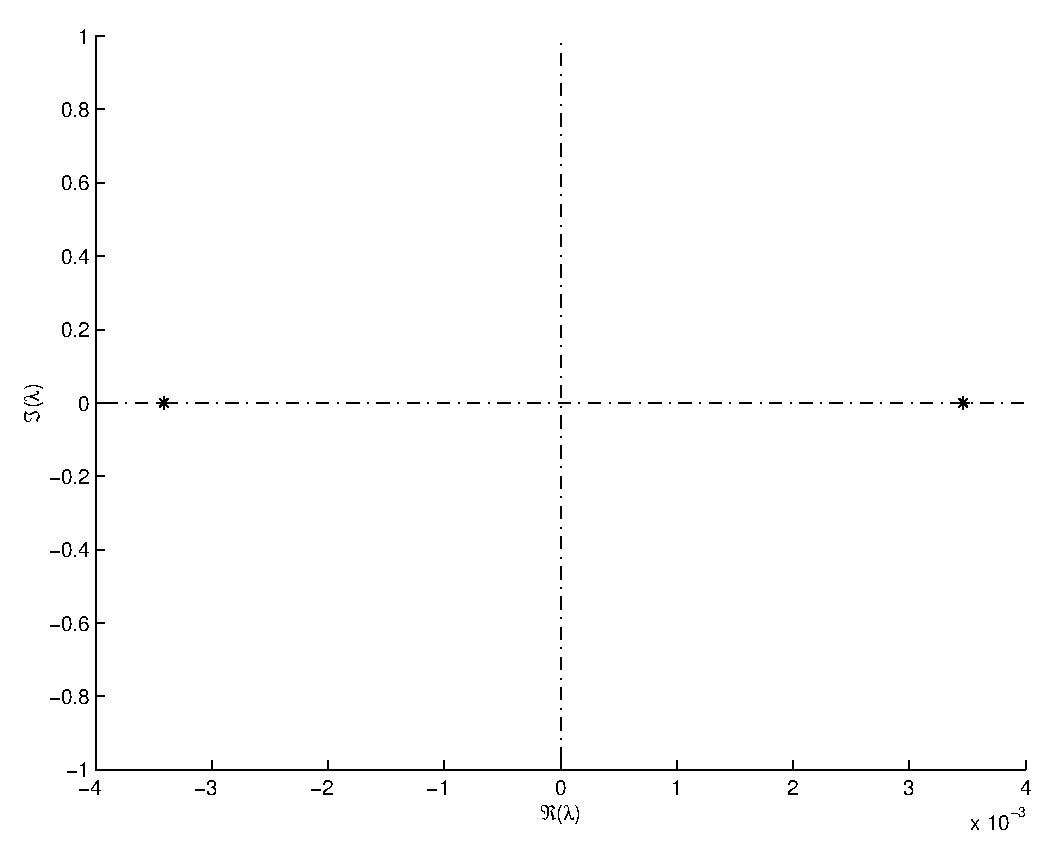
\includegraphics{fig/demo3-9.eps}}
\caption{\small Dominant eigenvalues of the saddle of the last point on the 
more accurate branch
of homoclinic orbits,
near a Takens-Bogdanov bifurcation.\label{demo3-9}}
\end{center}
\end{figure}

\section{Point manipulation}\label{point_manipulation}

Several of the point manipulation routines have already been used
in the previous section.
Here we outline their functionality and input and output parameters.
A brief description of parameters is also contained
within the source code and can be obtained in Matlab using the
$\parm{help}$ command. Note that a vector of zero elements 
corresponds to an empty matrix
(written in Matlab as $[]$).

{\small\begin{verbatim}
function [point,success]=p_correc(point0,free_par,step_cnd,method,adapt,previous,d_nr,tz)
\end{verbatim}}
\noindent Function \file{p\_correc} corrects a given point.
\begin{itemize}
\item $\parm{point0}$: initial, approximate solution point
as a point structure (see table \ref{point_structures}).
\item $\parm{free\_par}$: a vector of zero, one or more free parameters.
\item $\parm{step\_cnd}$: a vector of zero, one or more linear steplength
conditions. Each steplength condition is assumed fulfilled for
the initial point and hence only the coefficients of the condition
with respect to all unknowns are needed. These coefficients are passed 
as a point structure (see table \ref{point_structures}).
This means that, for, e.g., a steady state solution point $\parm{p}$ 
the $i$-th steplength
condition reads 
\[
\parm{step\_cnd(i).parameter}(\parm{p.parameter-point0.parameter})^T+
\parm{step\_cnd(i).x}^T(\parm{p.x-point0.x})=0,
\]
and similar formulas hold for the other solution types.
\item $\parm{method}$: a point method structure 
containing the method parameters (see table \ref{point_method_structures}).
\item $\parm{adapt}$ (optional): if zero or absent, do not use
adaptive mesh selection (for periodic solutions); 
if one, correct, use adaptive mesh selection and recorrect.
\item $\parm{previous}$ (optional): for periodic solutions and connecting 
orbits: if present and not empty, minimize phase 
shift with respect to this point. Note that this argument should always be
present when correcting solutions for sd-DDEs, since in that case the 
argument $\parm{d\_nr}$ always needs to be specified.  In the case of
steady state, fold or Hopf-like points, one can just enter an empty vector. 
\item $\parm{d\_nr}$: (only for equations with state-dependent delays) 
if present, number of a negative state-dependent delay. 
\item $\parm{tz}$: (only for equations with state-dependent delays 
and periodic solutions) if present, a periodic solution is computed 
such that $\tau(\parm{tz})=0$ and ${\d}\tau(\parm{tz})/{\d}t=0$,
where $\tau$ is a negative state-dependent delay with number
$\parm{d\_nr}$. For steady state solutions, a solution corresponding to
$\tau=0$ is computed. 
\item $\parm{point}$: the result of correcting $\parm{point0}$
using the method parameters, steplength condition(s) and free parameter(s)
given. Stability information present in $\parm{point0}$, 
is not passed onto $\parm{point}$.
If divergence occurred, $\parm{point}$ contains the final iterate.
\item $\parm{success}$: nonzero if convergence was detected (that is, if  
the requested accuracy has been reached). 
\end{itemize}

{\small\begin{verbatim}
function stability=p_stabil(point,method)
\end{verbatim}}
\noindent Function \file{p\_stabil} computes stability of a given point
by approximating its stability-determining eigenvalues.
\begin{itemize}
\item $\parm{point}$: a solution point as a point 
structure (see table \ref{point_structures}).
\item $\parm{method}$: a stability method structure 
(see table \ref{meth_stab_struct}).
\item $\parm{stability}$: the computed stability of the point
through a collection of approximated eigenvalues 
(as a structure described in table \ref{stab_structures}).
For steady state, fold and Hopf points both
approximations and corrections to the 
rightmost roots of the characteristic equation are provided.
For periodic
solutions approximations to the dominant Floquet multipliers are computed.
\end{itemize}

{\small\begin{verbatim}
function p_splot(point)
\end{verbatim}}
\noindent Function \file{p\_splot} plots the characteristic roots respectively
Floquet multipliers of a given point 
(which should contain nonempty stability information).
Characteristic root approximations and Floquet
multipliers are plotted using '$\times$',
corrected characteristic roots using '$*$'.

{\small\begin{verbatim}
function stst_point=p_tostst(point)
function fold_point=p_tofold(point)
function hopf_point=p_tohopf(point)
function [psol_point,stepcond]=p_topsol(point,ampl,degree,nr_int)
function [psol_point,stepcond]=p_topsol(point,ampl,coll_points)
function [psol_point,stepcond]=p_topsol(hcli_point)
function hcli_point=p_tohcli(point)
\end{verbatim}}
\noindent The functions \file{p\_tostst}, \file{p\_tofold}, \file{p\_tohopf},
\file{p\_topsol} and \file{p\_tohcli} convert a given point into 
an approximation of
a new point of the kind 
indicated by their name. They are used to switch from a steady state
point to a Hopf point or fold point, from a Hopf point to a fold point
or vice versa, from a (nearby double) Hopf point to the second Hopf
point, from a Hopf point to the emanating branch of periodic
solutions, from a periodic solution 
near a period doubling bifurcation to the period-doubled branch and from a 
periodic solution near a homoclinic orbit to this homoclinic orbit.  The 
function  \file{p\_tostst} is also capable of extracting the initial and 
final steady states from a connecting orbit.
When starting a periodic solution branch from a Hopf point, 
an equidistant mesh is produced 
with $\parm{nr\_int}$ intervals and piecewise polynomials of 
degree $\parm{col\_degree}$ and a steplength condition 
$\parm{stepcond}$ is returned which should be used 
(together with a corresponding free parameter) in correcting 
the returned point. This steplength condition (normally) prevents convergence
back to the steady state solution (as a degenerate periodic solution of amplitude
zero). When jumping to a period-doubled branch, a period-doubled solution
profile is produced using $\parm{coll\_points}$ for collocation points
and a mesh which is the (scaled) concatenation of two times the original mesh.
A steplength condition is returned which (normally) prevents convergence
back to the single period branch.
When jumping from a homoclinic orbit to a periodic solution, the steplength
condition prevents divergence, by keeping the period fixed.
When extracting the steady states from a connecting orbit, an array is returned
in which the first element is the initial steady state, and the second element
is the final steady state.

{\small\begin{verbatim}
function rm_point=p_remesh(point,new_degree,new_mesh)
\end{verbatim}}
\noindent Function \file{p\_remesh} changes the piecewise polynomial
representation of a given periodic solution point.
\begin{itemize}
\item $\parm{point}$: initial point, containing old mesh, old degree and
old profile.
\item $\parm{new\_degree}$: new degree of piecewise polynomials.
\item $\parm{new\_mesh}$: mesh for new representation of periodic solution
profile either as a (non-scalar) row vector of mesh points 
(both interval and representation
points, with the latter chosen equidistant between the
former, see section \ref{data_structures}) or as the new number of intervals.
In the latter case the new mesh is adaptively chosen based on the old
profile. 
\item $\parm{rm\_point}$: 
returned point containing new degree, new mesh and an 
appropriately interpolated
(but uncorrected!) profile.
\end{itemize} 

{\small\begin{verbatim}
function tau_eva=p_tau(point,d_nr,t)
\end{verbatim}}
\noindent Function \file{p\_tau} evaluates state-dependent delay(s) 
with number(s) $\parm{d\_nr}$. 
\begin{itemize}
\item $\parm{point}$: a solution point as a point structure.
\item $\parm{d\_nr}$: number(s) of delay(s) (in increasing order) 
to evaluate.
\item $\parm{t}$ (absent for steady state solutions and optional
for periodic solutions): mesh (a time point or a number of time 
points). If present,
delay function(s) are evaluated at the points of 
$\parm{t}$, otherwise at the
$\parm{point.mesh}$ (if $\parm{point.mesh}$ is empty, an equidistant 
mesh is used).
\item $\parm{tau\_eva}$: evaluated values of delays (at $\parm{t}$). 
\end{itemize}
\ 

The following routines are used within branch routines but
are less interesting for the general user.

{\small\begin{verbatim}
function sc_measure=p_measur(p,measure)
\end{verbatim}}
\noindent Function \file{p\_measur} computes the (scalar) measure $\parm{measure}$
of the given point $\parm{p}$ (see table \ref{measure_structure}). 

{\small\begin{verbatim}
function p=p_axpy(a,x,y)
\end{verbatim}}
\noindent Function \file{p\_axpy} performs the axpy-operation on
points. That is, it computes $\parm{p}=\parm{a}\parm{x}+\parm{y}$ where 
$\parm{a}$ is a scalar, and
$\parm{x}$ and $\parm{y}$ are two point structures of the same type.
$\parm{p}$ is the result of the operation on all appropriate
fields of the given points.
If $\parm{x}$ and $\parm{y}$ are 
solutions on different meshes, interpolation
is used and the result is obtained on the mesh of $\parm{x}$.
Stability information, if present, is not passed onto $\parm{p}$.

{\small\begin{verbatim}
function n=p_norm(point)
\end{verbatim}}
\noindent Function \file{p\_norm} computes some 
norm of a given point structure.

{\small\begin{verbatim}
function normalized_p=p_normlz(p)
\end{verbatim}}
\noindent Function \file{p\_normlz} performs some normalization on the
given point structure $\parm{p}$. In particular, fold, Hopf and 
connecting orbit
determining eigenvectors are scaled to norm 1.

{\small\begin{verbatim}
function [delay_nr,tz]=p_tsgn(point)
\end{verbatim}}
\noindent Function \file{p\_tsgn} detects a first negative state-dependent 
delay.
\begin{itemize}
\item $\parm{point}$: a solution point as a point structure.
\item $\parm{delay\_nr}$: number of the first (and only the first !) 
detected negative delay $\tau$.
\item $\parm{tz}$ (only for periodic solutions): $\parm{tz}\in [0,1]$ 
is a (time) point such that the delay function $\tau(t)$ has its 
minimal value near this point. To compute $\parm{tz}$, a refined mesh 
is used in the neighbourhood of the minimum of the delay function.
This point is later used to compute a periodic solution
such that $\tau(\parm{tz})=0$ and ${\d}\tau(\parm{tz})/{\d}t=0$. 
\end{itemize}

\section{Branch manipulation}\label{branch_manipulation}

Usage of most of
the branch manipulation routines has already been illustrated
in section \ref{demo}.
Here we outline their functionality and input and output variables.
As for all routines in the package, 
a brief description of the parameters is also contained
within the source code and can be obtained in Matlab using the
$\parm{help}$ command.

{\small\begin{verbatim}
function [c_branch,succ,fail,rjct]=br_contn(branch,max_tries)
\end{verbatim}}
\noindent The function \file{br\_contn} computes (or rather 
extends) a branch of solution
points. 
\begin{itemize}
\item $\parm{branch}$: initial branch 
containing at least two points and computation, stability and 
continuation method parameter
structures and a free parameter structure as described in 
table \ref{branch_struct}. 
\item $\parm{max\_tries}$:
maximum number of corrections allowed.
%\item $\parm{free\_par}$: vector of zero or more free parameter numbers. 
%\item $\parm{max\_step}$: vector of zero or more maximal parameter steps.
%Each row of 
%$\parm{max\_step}$ contains a parameter number (first element) and 
%a maximal step size
%allowed for that parameter (second element). These parameters should form a 
%(possibly empty) subset of the free parameters.
%\item $\parm{max\_bound}$: vector of zero or more minimal and maximal
%values for some parameters.
%Each row of the variable 
%$\parm{par\_bound}$ contains a parameter number (first element) and a 
%minimum (second element) and maximum (third element)
%value allowed for that parameter. If a boundary is crossed during 
%continuation,
%the point across the boundary is replaced with a point computed at the
%boundary and continuation is halted.
\item $\parm{c\_branch}$:
the branch returned contains a copy of the initial branch plus
the extra points computed (starting from the end of the point array in the
initial branch). 
\item $\parm{succ}$: number of successful corrections.
\item $\parm{fail}$: number of failed corrections.
\item $\parm{rjct}$: number of rejected points.
\end{itemize}
Note also that successfully computed points are normalized using the procedure
\file{p\_normlz} (see section \ref{point_manipulation}). 

{\small\begin{verbatim}
function br_plot(branch,x_measure,y_measure,line_type)
\end{verbatim}}
\noindent Function \file{br\_plot} plots a branch (in the current figure). 
\begin{itemize}
\item $\parm{branch}$: branch to plot (see table \ref{branch_struct}).
\item $\parm{x\_measure}$: (scalar) measure to produce plotting quantities
for the x-axis (see table \ref{measure_structure}). 
If empty, the point number is used to plot against.
\item $\parm{y\_measure}$: (scalar) measure to produce plotting quantities
for the y-axis (see table \ref{measure_structure}). 
If empty, the point number is used to plot against.
\item $\parm{line\_type}$ (optional): line type to plot with.
\end{itemize}

{\small\begin{verbatim}
function [x_measure,y_measure]=br_dfmsr(stability,branch)
function [x_measure,y_measure]=br_dfmsr(stability,par_list,kind)
\end{verbatim}}
\noindent Function \file{br\_measur} returns default measures
for plotting. 
\begin{itemize}
\item $\parm{stability}$: nonzero if measures are required to plot
stability information.
\item $\parm{branch}$: a given branch (see table \ref{branch_struct})
for which default measures should be constructed.
\item $\parm{par\_list}$: a list of parameters 
for which default measures should be constructed.
\item $\parm{kind}$: a point type 
for which default measures should be constructed.
\item $\parm{x\_measure}$: default scalar measure to use for the x-axis.
$\parm{x\_measure}$ is chosen as the first parameter which varies along
the branch or as the first parameter of $\parm{par\_list}$.
\item $\parm{y\_measure}$: default scalar measure to use for the y-axis.
If $\parm{stability}$ is zero, the following choices are
made for $\parm{y\_measure}$. For steady state solutions, 
the first component which varies along the branch; for fold and 
Hopf bifurcations 
the first parameter value (different from the one used
for $\parm{x\_measure}$) which varies along the branch. For 
periodic solutions, 
the amplitude of the fist varying component.
If $\parm{stability}$ is nonzero, $\parm{y\_measure}$ selects 
the real part of the characteristic roots (for steady state solutions, fold
and Hopf bifurcations) or
the modulus of the Floquet multipliers (for periodic solutions).
\end{itemize}

{\small\begin{verbatim}
function st_branch=br_stabl(branch,skip,recompute)
\end{verbatim}}
\noindent Function \file{br\_stabl} computes stability information
along a previously computed branch. 
\begin{itemize}
\item $\parm{branch}$: given branch (see table \ref{branch_struct}).
\item $\parm{skip}$: number of points to skip between stability computations.
That is, 
computations are
performed and stability field is filled in every $\parm{skip}+1$-th point.
\item $\parm{recompute}$: if zero, do not recompute stability information
present. If nonzero, discard and recompute old stability
information present (for points which were not skipped).
\item $\parm{st\_branch}$: a copy of the given branch whose (non-skipped) points 
contain a non-empty stability field with computed stability information
(using the method parameters contained in $\parm{branch}$).
\end{itemize}

{\small\begin{verbatim}
function t_branch=br_rvers(branch)
\end{verbatim}}
\noindent To continue a branch in the other direction (from the beginning instead
of from the end of its point array), \file{br\_rvers} reverses the
order of the points in the branches point array.

{\small\begin{verbatim}
function recmp_branch=br_recmp(branch,point_numbers)
\end{verbatim}}
\noindent Function \file{br\_recmp} recomputes part of a branch.
\begin{itemize}
\item $\parm{branch}$: initial branch (see table \ref{branch_struct}).
\item $\parm{point\_numbers}$ (optional): 
vector of one or more point numbers which should be
recomputed. Empty or absent if the complete point array should be recomputed.
\item $\parm{recmp\_branch}$: a copy of the initial branch with
points who were (successfully) recomputed replaced. If a recomputation fails, a
warning message is given and the old value remains present.
\end{itemize}
This routine can, e.g., be used after changing some method parameters within the branch
method structures.

{\small\begin{verbatim}
function [col,lengths]=br_measr(branch,measure)
\end{verbatim}}
\noindent Function \file{br\_selec} computes a measure along a branch.
\begin{itemize}
\item $\parm{branch}$: given branch (see table \ref{branch_struct}).
\item $\parm{measure}$: given measure (see table \ref{measure_structure}).
\item $\parm{col}$: the collection of measures taken along the
branch (over its point array) ordered row-wise. Thus, a column vector
is returned if $\parm{measure}$ is scalar. Otherwise,
$\parm{col}$ contains a matrix.
\item $\parm{lengths}$: vector of lengths of the measures along the branch.
If the measure is not scalar, it is possible
that its length varies along the branch (e.g.~when plotting rightmost
characteristic roots). In this situation $\parm{col}$ is a matrix 
with number of columns equal to the maximal length of the measures encountered.
Extra elements of $\parm{col}$ are automatically put to zero by Matlab.
$\parm{lengths}$ can then be used to prevent plotting of extra zeros.
\end{itemize}

\section{Numerical methods}\label{numerical_methods}\label{code_num_methods}

This section contains short descriptions of the numerical methods 
for DDEs and the method parameters used in {\DDEBIFCODE}. 
More details on the methods can be found in the
articles \cite{Luzy96,Enge99a,Enge99b,en_d01,engel01,homoclinic} 
or in \cite{Enge00}. For details on applying these methods to bifurcation
analysis of sd-DDEs see \cite{luz01}.

\subsection{Determining systems}\label{determining_systems}

Below we state the determining systems used to compute and
continue steady state solutions, steady state fold and Hopf 
bifurcations, periodic solutions and connecting orbits of systems of delay
differential equations.

For each determining system we mention the number of free 
parameters necessary to obtain (generically) isolated 
solutions. 
In the package,
the necessary number of free parameters
is further raised by the number of
steplength conditions plus the number of extra conditions used.
This choice ensures 
the use of square Jacobians during Newton iteration. 
If, on the other hand, the number of free parameters, 
steplength conditions and extra conditions
are not appropriately matched Newton iteration solves systems with a   
non-square Jacobian (for which Matlab uses an
over- or under-determined
least squares procedure). 
If possible, it is better to avoid such a situation.

\paragraph{Steady state solutions}
A steady state solution $x^*\in\RR^n$ is determined from the following
$n\times n$-dimensional determining system with no free parameters.
\begin{equation}\label{determ_stst}
f(x^*,x^*,\ldots,x^*,\eta)=0.
\end{equation}

\paragraph{Steady state fold bifurcations}
Fold bifurcations, $(x^*\in\RR^n,v\in\RR^n)$ are determined 
from the following
$2n+1\times 2n+1$-dimensional determining system using one free
parameter.
\begin{equation}\label{determ_fold}
\left\{
\begin{array}{l}
f(x^*,x^*,\ldots,x^*,\eta)=0 \\
\Delta(x^*,\eta,0)v=0\\
c^\T v-1=0
\end{array}
\right.
\end{equation}
Here, $c^\T v-1=0$ presents a suitable normalization of $v$.
The vector $c\in\RR^n$ is chosen as $c=v^{(0)}/({v^{(0)}}^\T v^{(0)})$,
where $v^{(0)}$ is the initial value of $v$.

\paragraph{Steady state Hopf bifurcations}
Hopf bifurcations, $(x^*\in\RR^n,v\in\CC^n,\omega\in\RR)$ are determined 
from the following
$2n+1\times 2n+2$-dimensional partially complex 
(and by this fact more properly called a 
$3n+2\times 3n+2$-dimensional)
determining system using one free parameter.
\begin{equation}\label{determ_hopf}
\left\{
\begin{array}{l}
f(x^*,x^*,\ldots,x^*,\eta)=0 \\
\Delta(x^*,\eta,\i\omega)v=0 \\
c^\H v-1=0
\end{array}
\right.
\end{equation}

\paragraph{Periodic solutions}
Periodic solutions are found as solutions 
$(u(s),\,s\in[0,1];T\in\RR)$ of the following
$(n(Ld+1)+1)\times (n(Ld+1)+1)$-dimensional system with no free parameters. 
\begin{equation}\label{determ_psol}
\left\{
\begin{array}{l}
\dot{u}(c_{i,j})=
Tf(u(c_{i,j}),u((c_{i,j}-\frac{\tau_1}{T})\,\mathrm{mod}\,1),\ldots,
u((c_{i,j}-\frac{\tau_m}{T})\,\mathrm{mod}\,1),\eta)=0, \\
\hspace{4cm}i=0,\ldots,L-1,\ j=1,\ldots,d \\
u(0)=u(1), \\
p(u)=0.
\end{array}
\right.
\end{equation}
Here $p$ represents the integral phase condition
\begin{equation}\label{integral_phase_cond}
\int_0^1\dot{u}(s)\Delta u(s)\d s=0,
\end{equation}
where $u$ is the current solution and $\Delta u$ its correction.
The collocation points are obtained as 
\[
c_{i,j}=t_i+c_j(t_{i+1}-t_i),\ i=0,\ldots,L-1,\ j=1,\ldots,d,
\]
from the interval points $t_i$, $i=0,\ldots,L-1$ and the
collocation parameters $c_j$, $j=1,\ldots,d$.
The profile $u$ is discretized as a piecewise polynomial as
explained in section \ref{data_structures}.
This representation has a discontinuous derivative at the 
interval points. If $c_{i,j}$ coincides with $t_i$ the right derivative
is taken in (\ref{determ_psol}), if it coincides with $t_{i+1}$ the left
derivative is taken. In other words the derivative taken at $c_{i,j}$
is that of $u$ restricted to $[t_i,t_{i+1}]$.

\paragraph{Connecting orbits}
Connecting orbits can be found as solutions of the following determining 
system with $s^+-s^-+1$ free parameters, where $s^+$ and $s^-$ denote the 
number of unstable eigenvalues of $x^+$ and $x^-$ respectively. 
\begin{equation}\label{determ_hcli}
\left\{
\begin{array}{l}
\dot{u}(c_{i,j})=
Tf(u(c_{i,j}),u(c_{i,j}-\frac{\tau_1}{T}),\ldots,
u(c_{i,j}-\frac{\tau_m}{T}),\eta)=0, \\
\hspace{4cm}(i=0,\ldots,L-1,\ j=1,\ldots,d) \\ 
u(\tilde{c})=x^{-}+\epsilon
\sum_{k=1}^{s^{-}}\alpha_{k}v_{k}^{-}e^{\lambda_{k}^{-}T\tilde{c}}, \qquad \tilde{c}<0\\
f(x^{-},x^{-},\eta)=0\\
f(x^{+},x^{+},\eta)=0\\
\Delta(x^{-},\lambda_k^-,\eta) v_{k}^{-}=0 \\
c_k^{H}v_{k}^{-}-1=0\\
\hspace{4cm} (k=1,\ldots,s^{-})\\
\Delta^{H}(x^{+},\lambda_k^+,\eta)w_{k}^{+}=0 \\
d_k^{H}w_{k}^{+}-1=0\\
\hspace{4cm} (k=1,\ldots,s^{+})\\
{w_{k}^{2}}^{H}(u(1)-x^{+})+\sum_{i=1}^{G}g_i{w_{k}^{+}}^{H}e^{-\lambda_{k}^{+}
(\theta_i+\tau)}A_{1}(x^{+},\eta)
\left(u(1+\frac{\theta_i}{T})-x^{+}\right)=0\\
\hspace{4cm}( k=1,\ldots,s^+)\\
 u(0)=x^{-}+\epsilon\sum_{i=1}^{s^{-}}\alpha_{k}v_{k}^{-}\\
\sum_{i=1}^{s^-}|\alpha_{k}|^{2}=1\\
p(u,\eta)=0
\end{array}
\right.
\end{equation}
We choose the same phase condition as for periodic solutions
and similar normalization of $v_k^-$ and $w+k^+$ as in (\ref{determ_hopf}).

\paragraph{Point method parameters}
The point method parameters (see table \ref{point_method_structures}) 
specify the following options.
\begin{itemize}
\item $\parm{newton\_max\_iterations}$: maximum number of Newton
iterations.    
\item $\parm{newton\_nmon\_iterations}$: during a first phase of 
$\parm{newton\_nmon\_iterations}+1$
Newton iterations the norm of the residual is allowed
to increase. After these iterations, corrections are halted
upon residual increase.
\item $\parm{halting\_accuracy}$: corrections are halted when
the norm of the last computed 
residual is less than or equal to $\parm{halting\_accuracy}$ 
is reached.  
\item $\parm{minimal\_accuracy}$: a corrected point is accepted
when the norm of the last computed residual is less than or equal
to $\parm{minimal\_accuracy}$.     
\item $\parm{extra\_condition}$: this parameter is nonzero
when extra conditions are provided in a routine \file{sys\_cond.m}
which should border the determining systems during corrections.
The routine accepts the current point as input and
produces an array of condition residuals and corresponding
condition derivatives (as an array of point structures) as
illustrated below (\S\ref{extra_cond}).
\item $\parm{print\_residual\_info}$: when nonzero, the Newton
iteration number and resulting
norm of the residual are printed to the screen during corrections.
\end{itemize}
For periodic solutions and connecting orbits,
the extra mesh parameters 
(see table \ref{psol_extra_p_struct}) provide the following
information.
\begin{itemize}
\item $\parm{phase\_condition}$: when nonzero the integral phase condition
(\ref{integral_phase_cond}) is used.        
\item $\parm{collocation\_parameters}$: this parameter contains user given
collocation parameters. When empty, Gauss-Legendre collocation points are
chosen.    
\item $\parm{adapt\_mesh\_before\_correct}$: before correction and if
the mesh inside the point is nonempty, adapt
the mesh every $\parm{adapt\_mesh\_before\_correct}$ points.
E.g.: if zero, do not adapt; if one, adapt every point; if two adapt the
points with odd point number.
\item $\parm{adapt\_mesh\_after\_correct}$: similar to 
$\parm{adapt\_mesh\_before\_correct}$ but adapt mesh after 
successful corrections and correct again. 
\end{itemize}

\subsection{Extra conditions}\label{extra_cond}

When correcting a point or computing a branch, it is possible to
add one or more extra conditions and corresponding 
free parameters to the determining systems presented
earlier. These extra conditions should be implemented using
a file \file{sys\_cond.m} in the directory of the system definition
and setting the method parameter $\parm{extra\_condition}$ to 1
(cf.\ table \ref{point_method_structures}).
The function \file{sys\_cond} accepts the current point as input and
produces a residual and corresponding
condition derivatives (as a point structure) per extra condition.

As an example, suppose we want to compute a branch of
periodic solutions of system (\ref{example_sys}) subject to the following
extra conditions 
\[
\left\{
\begin{array}{l}
T=200, \\
a_{12}^2+a_{21}^2=1,
\end{array}
\right.
\]
that is, we wish to continue a branch with fixed period $T=200$
and parameter dependence $a_{12}^2+a_{21}^2=1$.
The following routine implements these conditions by 
evaluating and returning each residual for the given point
and the derivatives of the conditions w.r.t.\ all unknowns
(that is, w.r.t.\ to all the components of the point structure).

\begin{boxit}{9.5cm}
{\small\begin{verbatim}
function [resi,condi]=sys_cond(point)

% kappa beta a12 a21 tau1 tau2 tau_s

if point.kind=='psol'
  % fix period at 200:
  resi(1)=point.period-200;
  % derivative of first condition wrt unknowns:
  condi(1)=p_axpy(0,point,[]);
  condi(1).period=1;
  % parameter condition:
  resi(2)=point.parameter(3)^2+point.parameter(4)^2-1;
  % derivative of second condition wrt unknowns:
  condi(2)=p_axpy(0,point,[]);
  condi(2).parameter(3)=2*point.parameter(3);
  condi(2).parameter(4)=2*point.parameter(4);
else
  error('SYS_COND: point is not psol.');
end;

return;
\end{verbatim}}
\end{boxit}

\subsection{Continuation}\label{continuation}

During continuation, a branch is extended by a combination
of predictions and corrections.
A new point is predicted based on previously computed points
using
secant prediction 
over an appropriate steplength. The prediction is then corrected
using the
determining systems (\ref{determ_stst}), (\ref{determ_fold}), 
(\ref{determ_hopf}), (\ref{determ_psol}) or   
(\ref{determ_hcli}) bordered with a steplength condition
which requires orthogonality 
of the correction to the secant vector.
Hence one extra free parameter is necessary compared to the 
numbers mentioned in the previous section.
 
The following continuation and steplength determination 
strategy is used.
If the last point was successfully computed, the steplength
is multiplied with a given, constant factor greater than 1.
If corrections diverged or if the corrected point was rejected
because its accuracy was not acceptable,
a new point is predicted, using linear interpolation, halfway between the
last two successfully computed branch points.
If the correction of this point succeeds, 
it is inserted in the point array of the branch (before the
previously last computed point). 
If the correction of the interpolated point fails again, 
the last successfully computed branch point is rejected (for fear
of branch switch) and the interpolation procedure 
is repeated between the (new) last two
branch points. Hence, if, after a failure, the interpolation 
procedure succeeds, the steplength is approximately divided by 
a factor two. Test results indicate that this procedure is quite
effective and proves an efficient alternative to 
using only (secant) extrapolation with steplength control.
The reason for this is mainly that
the secant extrapolation direction is not influenced by halving
the steplength but it is by inserting a newly computed point in between
the last two computed points.

The continuation method parameters (see table \ref{continuation_structure})
have the following meaning.
\begin{itemize}
\item $\parm{plot}$: if nonzero, plot predictions and corrections
during continuation.
\item $\parm{prediction}$: this parameter should be 1, indicating
that secant prediction is used (being currently the only
alternative).
\item $\parm{steplength\_growth\_factor}$: grow the steplength with
this factor in every step except during interpolation.
\item $\parm{plot\_progress}$: if nonzero, plotting is visible during
continuation process. If zero, only the final result is drawn.
\item $\parm{plot\_measure}$: if empty use default measures to plot.
Otherwise $\parm{plot\_measure}$ contains two fields, 'x' and 'y',
which contain measures (see table \ref{measure_structure}) for use in plotting during
continuation.
\item $\parm{halt\_before\_reject}$: If this parameter is nonzero,
continuation is halted whenever (and instead of) rejecting a
previously accepted point based on the above strategy.
\end{itemize}

\subsection{Roots of the characteristic equation}\label{root_char_equa_gio_label}

Roots of the characteristic equation are
approximated using a linear multi-step (LMS-) method
applied to (\ref{the_var_equa}).

Consider the linear $k$-step formula
\begin{equation}\label{lms_method}
\sum_{j=0}^k\alpha_j y_{L+j}=h\sum_{j=0}^k\beta_j f_{L+j}.
\end{equation}
Here, $\alpha_0=1$, $h$ is a (fixed) step size and 
$y_j$ presents the numerical approximation of $y(t)$ at the mesh
point $t_j\defeq jh$.
The right hand side
$f_j\defeq f(y_j,\tilde{y}(t_j-\tau_1),\ldots,\tilde{y}(t_j-\tau_m))$ 
is computed using approximations $\tilde{y}(t_j-\tau_1)$ 
obtained from $y_i$ in the past, $i<j$.
In particular, the use of so-called Nordsieck interpolation, leads to
\begin{equation}\label{past_terms}
\tilde{y}(t_j+\epsilon h)=\sum_{l=-r}^s P_l(\epsilon)y_{j+l},\ \epsilon \in [0,1).
\end{equation}
using
\[
P_l(\epsilon)\defeq\prod_{k=-r,\,k\neq l}^s\frac{\epsilon-k}{l-k}.
\]

The resulting method is explicit whenever $\beta_0=0$ and 
$\min{\tau_i}>sh$.
That is, $y_{L+k}$ can then directly be computed from (\ref{lms_method})
by evaluating
\[
y_{L+k}=-\sum_{j=0}^{k-1}\alpha_j y_{L+j}+h\sum_{j=0}^k\beta_j f_{L+j}.
\]
whose right hand side depends only on $y_j$, $j<L+k$.

For the linear variational equation (\ref{the_var_equa})
around a steady state solution $x^*(t)\equiv x^*$
we have
\begin{equation}\label{linear_rhs}
f_j=A_0y_j+\sum_{i=0}^mA_i\tilde{y}(t_j-\tau_i)
\end{equation}
where we have omitted the dependency of $A_i$ on $x^*$.
The stability of the difference scheme (\ref{lms_method}), (\ref{linear_rhs})
can be evaluated by setting $y_j=\mu^{j-L_{\min}}$, $j=L_{\min},\ldots,L+k$ 
where $L_{\min}$ is the 
smallest index used, taking the determinant of (\ref{lms_method})
and computing the roots $\mu$. If the roots of the
polynomial in $\mu$ all have modulus smaller than 1, the trajectories
of the LMS-method converge to zero. 
If roots exist with modulus greater then trajectories exist
which grow unbounded.

Since the LMS-method forms an approximation of
the time integration operator over the time step $h$, so do the 
roots $\mu$ approximate the eigenvalues of $S(h,0)$.
The eigenvalues of $S(h,0)$ are exponential transforms of
the roots $\lambda$ of the characteristic 
equation (\ref{the_char_eq}),
\[
\mu=\exp(\lambda h).
\]
Hence, once $\mu$ is found, $\lambda$ can be extracted using,
\begin{equation}\label{extract_real_part}
\Re(\lambda)=\frac{\ln(|\mu|)}{h}.
\end{equation}
The imaginary part of $\lambda$ is found modulo $\pi/h$, using
\begin{equation}\label{extract_imag_part}
\Im(\lambda)\equiv\frac{\arcsin(\frac{\Im(\mu)}{|\mu|})}
{h}\!\!\!\!\pmod{\frac{\pi}{h}}.
\end{equation}
For small $h$, $0<h\ll 1$, the smallest representation 
in (\ref{extract_imag_part})
is assumed the most accurate one (that is, we let $\arcsin$
map into $[-\pi/2,\pi/2]$).

The parameters $r$ and $s$ (from formula (\ref{past_terms}))
are chosen such that $r\leq s\leq r+2$ (see \cite{Hong96}).
The choice of $h$ is based on the related 
heuristic outlined in \cite{engel01}.

Approximations for the rightmost roots $\lambda$ obtained
from the LMS-method using (\ref{extract_real_part}), 
(\ref{extract_imag_part}) can be corrected
using a Newton process on the system,
\begin{equation}\label{determ_root}
\left\{
\begin{array}{l}
\Delta(\lambda)v=0 \\
c^\T v-1=0
\end{array}
\right.
\end{equation}
A starting value for $v$ is the eigenvector of 
$\Delta(\lambda)$ corresponding to its smallest eigenvalue (in modulus).

Note that the collection of successfully corrected roots presents 
more accurate yet less robust information than the set of uncorrected
roots. Indeed, attraction domains of roots of equations 
like (\ref{determ_root})
can be very small and hence
corrections may diverge or
approximations of different roots may be corrected to a single 'exact' root 
thereby missing part of the spectrum.
The latter does not occur when computing the (full) spectrum
of a discretization of $S(h,0)$.

Stability information is kept in the structure of table \ref{stab_structures} 
(left). The time step used is kept in field $\parm{h}$. Approximate
roots are kept in field $\parm{l0}$, corrected roots in field $\parm{l1}$.
If unconverged corrected roots are discarded, field $\parm{n1}$
is empty.
Otherwise, the number of Newton iterations used is kept for 
each root in the corresponding position of $\parm{n1}$. Here, $-1$ 
signals that 
convergence to the required accuracy
was not reached.
The stability method parameters (see table \ref{meth_stab_struct} (top)) 
now have the following meaning. 
\begin{itemize}
\item $\parm{lms\_parameter\_alpha}$: LMS-method parameters $\alpha_j$ 
ordered from past to present, $j=0,1,\ldots,k$.
\item $\parm{lms\_parameter\_beta}$: LMS-method parameters $\beta_j$ 
ordered from past to present, $j=0,1,\ldots,k$.
\item $\parm{lms\_parameter\_rho}$: safety radius
$\rho_{\mathrm{LMS},\epsilon}$ of the LMS-method stability region.
For a precise definition, see \cite[\S III.3.2]{Enge00}.
\item $\parm{interpolation\_order}$: order of the interpolation in the
past, $r+s=\parm{interpolation\_order}$.
\item $\parm{minimal\_time\_step}$: minimal time step relative to maximal
delay, $\frac{h}{\tau}\geq\parm{minimal\_time\_step}$.
\item $\parm{maximal\_time\_step}$: maximal time step relative to maximal
delay, $\frac{h}{\tau}\leq\parm{minimal\_time\_step}$. 
\item $\parm{max\_number\_of\_eigenvalues}$: maximum number of rightmost
eigenvalues to keep.
\item $\parm{minimal\_real\_part}$: choose $h$ such as to approximate
eigenvalues with $\Re(\lambda)\geq \parm{minimal\_real\_part}$ well,
discard eigenvalues with 
$\Re(\lambda)<\parm{minimal\_real\_part}$.
If $h$ is smaller than its minimal value, it is set to the minimal
value and a warning is uttered. If it is larger than its maximal value
it is reduced to that number without warning.
If minimal and maximal value coincide, $h$ is set to this value
without warning.  
If $\parm{minimal\_real\_part}$ is empty, the value 
$\parm{minimal\_real\_part}=\frac{1}{\tau}$ is used.
\item $\parm{max\_newton\_iterations}$: maximum number of Newton
iterations during the correction process (\ref{determ_root}).
\item $\parm{root\_accuracy}$: required accuracy of 
the norm of the residual of (\ref{determ_root}) during
corrections.
\item $\parm{remove\_unconverged\_roots}$: if this parameter is zero,
unconverged roots are discarded (and stability field $\parm{n1}$ is empty). 
\item $\parm{delay\_accuracy}$ (only for state-dependent delays): if
the value of a state-dependent delay is less than
$\parm{delay\_accuracy}$, the stability is not computed.
\end{itemize}

\subsection{Floquet multipliers}

Floquet multipliers are computed as eigenvalues of
the discretized time integration operator $S(T,0)$.
The discretization is obtained using the collocation equations 
(\ref{determ_psol}) without the modulo operation
(and without phase and periodicity condition). 
From this system a discrete, linear map is
obtained between the variables presenting the segment 
$[-\tau/T,0]$ and those presenting the segment $[-\tau/T+1,1]$.
If these variables overlap, part of the map is just a time
shift.

Stability information is kept in the structure of table \ref{stab_structures} 
(right). Approximations to the Floquet multipliers 
are kept in field $\parm{mu}$.
The stability method parameters (see table \ref{meth_stab_struct} (bottom)) 
have the following meaning. 
\begin{itemize}
\item $\parm{collocation\_parameters}$: user given
collocation parameters or empty for Gauss-Legendre collocation points.      
\item $\parm{max\_number\_of\_eigenvalues}$: maximum number of multipliers
to keep.
\item $\parm{minimal\_modulus}$: discard multipliers with
$|\mu|<\parm{minimal\_modulus}$.
\item $\parm{delay\_accuracy}$ (only for state-dependent delays): if
the value of a state-dependent delay is less than
$\parm{delay\_accuracy}$, the stability is not computed.
\end{itemize}

\section{Concluding comments}\label{limits_sec}

The first aim of {\DDEBIFCODE} is to provide a portable,
user-friendly 
tool for numerical bifurcation analysis 
of steady state solutions and periodic solutions of systems
of delay differential equations of the kinds (\ref{the_dde_type})
and (\ref{the_dde_type2}).
Part of this goal was fulfilled through choosing
the portable, programmer-friendly environment
offered by Matlab.
Robustness with respect to the numerical approximation
is achieved through automatic steplength
selection in approximating the rightmost characteristic roots
and through collocation using piecewise polynomials combined
with adaptive mesh selection.

Although
the package has been successfully tested on a number of realistic examples,
a word of caution may be appropriate. First of all, the package
is essentially a research code (hence we accept no
reliability) in a quite unexplored area of current
research. In our experience up to now, 
new examples did not fail to produce
interesting theoretical questions (e.g., concerning homoclinic
or heteroclinic solutions) many of which
remain unsolved today. 
Unlike for ordinary differential equations, discretization
of the state space is unavoidable during computations on
delay equations. Hence the user of the package is 
strongly advised 
to investigate the effect of discretization using tests on different
meshes and with different method parameters; and, if
possible, to compare with analytical results and/or results obtained
using simulation.

Although there are no 'hard' limits programmed in the package (with respect
to system and/or mesh sizes),
the user will notice the rapidly increasing computation time
for increasing system dimension and mesh sizes.
This exhibits itself most profoundly in the stability and
periodic solution computations. 
Indeed, eigenvalues are computed from large sparse matrices
without exploiting sparseness and the  
Newton procedure for periodic solutions is implemented using direct methods.
Nevertheless the current version is sufficient to perform
bifurcation analysis of systems with reasonable properties
in reasonable execution times. 
Furthermore we hope future versions will include routines 
which scale better with the size of the problem.

Other future plans include a graphical user interface and
the extension to other types
of delay equations such as distributed delay and
neutral functional differential equations.

\section*{Acknowledgements}

This report presents results of the research project 
OT/98/16, funded by the Research Council K.U.Leuven;
of the research project G.0270.00 funded 
by the Fund for Scientific Research - Flanders (Belgium) and of the 
research project IUAP P4/02 funded by the programme
on Interuniversity Poles of Attraction, initiated by the Belgian State,
Prime Minister's Office for Science, Technology and Culture.
K.~Engelborghs is a Postdoctoral Fellow of the Fund for Scientific 
Research - Flanders (Belgium).

Thanks to D.~Roose for being the promoter of
the research that culminated into this package.

\bibliographystyle{plain}

\bibliography{manual}

\newpage

\section*{Appendix A: List of files}

Version 2.00 of {\DDEBIFCODE} contains the following files.
\begin{center}
\begin{tabular}{lllll}
Layer 0   & Layer 1   & Layer 2   & Layer 3   & Extra     \\ \hline
sys\_cond & auto\_cnt & p\_axpy   & br\_contn & df\_brnch \\
sys\_deri & auto\_eqd & p\_correc & br\_measr & df\_deriv \\
sys\_dtau & auto\_msh & p\_measur & br\_plot  & df\_derit \\
sys\_ntau & auto\_ord & p\_norm   & br\_recmp & df\_measr \\
sys\_init & fold\_jac & p\_normlz & br\_refin & df\_mthod \\
sys\_rhs  & hcli\_eva & p\_pplot  & br\_rvers & demo1     \\
sys\_tau  & hcli\_jac & p\_remesh & br\_stabl & sd\_demo  \\
          & hopf\_jac & p\_secant &           & hom\_demo  \\ 
          & mult\_app & p\_splot  &           & genr\_sys.mth \\
          & mult\_dbl & p\_stabil \\
          & mult\_int & p\_tau    \\
          & mult\_plt & p\_tofold \\
          & poly\_del & p\_tohcli \\
          & poly\_dla & p\_tohopf \\
          & poly\_d2l & p\_topsol \\
          & poly\_elg & p\_tostst \\
          & poly\_gau & p\_tsgn   \\
          & poly\_lgr \\ 
          & poly\_lob \\
          & psol\_eva \\ 
          & psol\_jac \\
          & psol\_msh \\ 
          & root\_app \\
          & root\_cha \\
          & root\_int \\
          & root\_nwt \\
          & root\_plt \\
          & stst\_jac \\
          & time\_h   \\
          & time\_lms \\
          & time\_nrd \\
          & time\_saf
\end{tabular}
\end{center}

\newpage

\section*{Appendix B: Obtaining the package}

{\DDEBIFCODE} is freely available for scientific (non-commercial)
use. It was started by the first author as a part of his PhD at
the Computer Science Department of the K.U.Leuven under supervision
of Prof.\ D.\ Roose.

The following terms cover the use of the software package {\DDEBIFCODE}:
\begin{enumerate}
\item The package {\DDEBIFCODE} can be used only for the purpose of internal
research excluding any commercial use of the package {\DDEBIFCODE} as such
or as a part of a software product.
\item {\scshape K.U.Leuven, Department of Computer Science} shall for all
purposes be considered the owner of {\DDEBIFCODE} and of all copyright,
trade secret, patent or other intellectual property rights therein.
\item The package {\DDEBIFCODE} is provided on an "as is" basis and
for the purposes described in paragraph 1 only. In no circumstances
can {\scshape K.U.Leuven} be held liable for any deficiency, fault
or other mishappening with regard to the use or performance of
the package {\DDEBIFCODE}.
\item All scientific publications, for which the package {\DDEBIFCODE}
has been used, shall mention usage of the package {\DDEBIFCODE},
and shall refer to the following publication:
\begin{quote}
K.~Engelborghs, T.~Luzyanina, G.~Samaey. DDE-BIFTOOL\ v.~2.00 user manual: 
a Matlab package for bifurcation analysis
of delay differential equations. Technical Report TW-330, Department of
Computer Science, K.U.Leuven, Leuven, Belgium, 2001.
\end{quote}
\end{enumerate}

Upon acceptance of the above terms, one can obtain the package
{\DDEBIFCODE} (version 2.00) 
by mailing your full name, affiliation and 
address to \verb#koen.engelborghs@cs.kuleuven.ac.be#.
The package will then be forwarded to you.

\end{document}
